% Copyright (c) 2004 Mikko Rantalainen
% Permission is granted to copy, distribute and/or modify this
% document under the terms of the GNU Free Documentation
% License, Version 1.2 or any later version published by the
% Free Software Foundation; with no Invariant Sections, no
% Front-Cover Texts, and no Back-Cover Texts.  A copy of the
% license is included in the section entitled "GNU Free
% Documentation License".

\documentclass[finnish,latin1,newtitle]{gradu2}

%%%%%%%%%%%%%%%%%%%%%%%%%%%%%%%%%%%%%%%%%%%%%%%%%%
%	M E T A
%%%%%%%%%%%%%%%%%%%%%%%%%%%%%%%%%%%%%%%%%%%%%%%%%%

\title{Aidosti selaink�ytt�iset sovellukset,\\ esimerkkin� Peda.net}
\translatedtitle{Truly Browser Accessible Applications, case Peda.net}

\tiivistelma{T�m� pro gradu -tutkielma selvitt��, kuinka
www-selaimella toimivat k�ytt�liittym�t eroavat perinteisist�,
k�ytt�liittymiss� natiivisti toimivista ohjelmista ja kuinka t�m�
tulisi ottaa huomioon k�ytt�liittym�n suunnittelussa ja toteutuksessa.
Vastapainona teorialle kuvailen Peda.net -projektissa ja -hankkeessa
tekemi�ni selaink�ytt�isi� sovelluksia ja niiss� tehtyj� ratkaisuja ja
kompromisseja.}

\avainsanat{k�ytt�liittym�, k�ytett�vyys, selain, www, verkkosovellus,
HTML, CSS, XHTML, XML}

\abstract{This Master's Thesis investigates how web based user
interfaces differ from traditional native user interfaces and how this
relates to the design and implementation of web applications. In
addition to theory, I will describe some web browser accessible
applications that I have developed in Peda.net project. I will discuss
technical decisions, compromises and advancements in the more recent
applications.}

\keywords{user interface, usability, browser, www, web application,
HTML, CSS, XHTML, XML}


\setauthor{Mikko}{Rantalainen}
%\setdate{01}{06}{2004}
%\tyyppi{Pro Gradu -ehdotus}
%\type{A Master's Thesis Candidate}

\yhteystiedot{Mikko Rantalainen \texttt{<mikko.rantalainen@iki.fi>}}
\license{Permission is granted to copy, distribute and/or modify this document under the terms of the GNU Free Documentation License,, Version 1.2 or any later version published by the Free Software Foundation}

% k�ytet��n pakettia amssymb mathbb{} funktion hakuun
%\usepackage{amssymb}
\usepackage{listings}
\usepackage{graphicx}

\newcommand{\strong}[1]{\textbf{#1}}
\newcommand{\class}[1]{\texttt{#1}}
\newcommand{\method}[1]{\texttt{#1}}
\newcommand{\command}[1]{\texttt{#1}}
\newcommand{\keyword}[1]{\texttt{#1}}
\newcommand{\element}[1]{\texttt{#1}}
\newcommand{\attribute}[1]{\texttt{#1}}
\newcommand{\tag}[1]{\texttt{#1}}
\newcommand{\alt}[1]{\textsl{#1}}
\newcommand{\term}[1]{\textsl{#1}}
\newcommand{\code}[1]{\texttt{#1}}

\newenvironment{cmds}
  {\begin{description}\renewcommand{\makelabel}[1]{\texttt{\textbackslash##1}\hfill}}
  {\end{description}}

\newenvironment{terms}
  {\begin{description}}
  {\end{description}}

\newenvironment{kuva}
  {\begin{figure}[hb!t]
  \begin{center}}
  {\end{center}
  \end{figure}}

% all these settings require Listings package version 1.0. Usually only version 0.20 is available.
%\lstset{extendedchars=true,basicstyle=\ttfamily,firstnumber=1,breaklines=true,xleftmargin=6mm}
\lstset{extendedchars=true,basicstyle=\ttfamily}

\hyphenation{
mo-zilla net-scape in-ter-net ex-plor-er XHTML HTML SMIL SVG
tuot-ta-mis-ym-p�-ris-t�
}


% usage:
% \mycite[page no]{books bibname}{cited text}
% or
% \mycite{source}{cited text}
\def\myempty{}
\newcommand*{\mycite}[3][]{\begin{quote} \textit{``#3''}
    \def\temp{#1}%
    \ifx\temp\myempty \cite{#2}
    \else \cite[#1]{#2}
    \fi  \end{quote}}

\newenvironment{ul}
  {\begin{itemize}}
  {\end{itemize}}

\newenvironment{ol}
  {\begin{enumerate}}
  {\end{enumerate}}

% compact list without extra spacing
\newenvironment{ul*}%
  {\begin{itemize}%
    %\setlength{\topsep}{0pt}%
    \setlength{\itemsep}{0pt}%
    \setlength{\parskip}{0pt}}%
  {\end{itemize}}

% compact list without extra spacing
\newenvironment{ol*}%
  {\begin{enumerate}%
    %\setlength{\topsep}{0pt}%
    \setlength{\itemsep}{0pt}%
    \setlength{\parskip}{0pt}}%
  {\end{enumerate}}

% description/definition list
\newenvironment{dl}
  {\begin{description}}
  {\end{description}}

%\usepackage{savetrees}

% salli rumat tavutukset ja rivitykset
%\sloppy
% vaadi siistit tavutukset ja rivitykset
\fussy


% http://www.wlug.org.nz/PdfLatexNotes

% if using pdflatex, we must use our .pdf images instead of .(e?)ps
\ifx\pdfoutput\undefined
\else
\DeclareGraphicsExtensions{.pdf,.gif,.jpg,.png} % the formats we have images in
\pdfadjustspacing=1
\fi


%%%%%%%%%%%%%%%%%%%%%%%%%%%%%%%%%%%%%%%%%%%%%%%%%%
%	D O C U M E N T
%%%%%%%%%%%%%%%%%%%%%%%%%%%%%%%%%%%%%%%%%%%%%%%%%%

\begin{document}

\preface

Kuulen joskus kerrottavan, ett� jokin sovellus on \emph{selaink�ytt�inen}. T�ss� yhteydess� termi tarkoittaa mielest�ni tietokoneohjelmaa, jonka k�ytt�liittym� on rakennettu toimimaan www-selaimella. Er��t tahot tuntuvat kuitenkin k�ytt�v�n termi� my�s esim. Java-ohjelmointikielell� toteutetuista ohjelmista, jotka vain k�ynnistet��n suoraan selainikkunasta. Minun mielest�ni tuollainen ohjelma ei ole selaink�ytt�inen, sill� esimerkiksi puhelimessani voi olla www-selain, mutta silti tuollainen ohjelma ei toimisi siin�. Selv�sti tuollainen ohjelma ei siis ole selaink�ytt�inen! T�m� tutkielma keskittyykin \emph{aidosti} selaink�ytt�isiin sovelluksiin. Sellaisiin, jotka toimivat miss� tahansa ymp�rist�ss� toimivissa HTML-selaimissa.


\mainmatter % reset page numbering to arabic, print TOC

\chapter{Johdanto}

\begin{chapterquote}{Jakob Nielsen's Alertbox, 2001-08-05} To design an
easy"-to"-use interface, pay attention to what users do, not what they
say. Self"-reported claims are unreliable, as are user speculations
about future behavior. \end{chapterquote}

Voidaan perustellusti v�itt��, ett� jokainen www"-sivuja tehokkaasti
lukeva ja verkossa olevaa materiaalia hyv�kseenk�ytt�v� henkil� on
tietoinen www"-selainten perusominaisuuksista. T�rkein, erityisesti
www"-selaimelle tyypillinen toiminto on linkkien seuraaminen.
Kokeneelle k�ytt�j�lle \emph{takaisin}"-toiminto, jolla voidaan
sivuhistoriassa palata edelliselle sivulle, on miltei yht� arvokas. Jos
www"-selainta k�ytt�v� henkil� huomaa esimerkiksi sis�llysluettelosta
jonkin kohdan valittuaan, ett� valinta oli v��r�, voi h�n t�m�n
toiminnon avulla v�litt�m�sti palata takaisin sis�llysluetteloon
miettim�tt� olisiko valinnan seurauksena annetulla sivulla ollut jokin
keino siirty� sis�llysluetteloon.

V�litt�m�sti linkkien seuraamisen j�lkeen www"-sivuja k�ytt�v� henkil�
oppiikin takaisin"-toiminnon k�yt�n. Jos verkossa linkkien
seuraamistaito vastaa lukemaan oppimista, niin takaisin"-toiminnon
k�ytt� vastaa kirjoittamista. T�st� huolimatta selaink�ytt�isess�
sovelluksessa takaisin"-toiminnon k�ytt�minen aiheuttaa liian usein
ohjelman rikkoutumisen.\footnote{Muita usein tavallisten sivujen
yhteydess� k�ytettyj� toimintoja, jotka eiv�t toimi monessa
selaink�ytt�isess� sovelluksessa, ovat mm. linkin avaaminen toisessa
ikkunassa ja kirjanmerkin luominen.} Selaink�ytt�isten ohjelmien
kehitt�jien yleinen kysymys onkin, \emph{kuinka takaisin"-toiminnon
k�ytt� voitaisiin est��}, kun oikea kysymys olisi, \strong{miksi} se
pit�isi est��. Jos k�ytt�j� selv�sti haluaa suorittaa kyseisen
toiminnon, niin eik� jotain pit�isi tehd� sen hyv�ksi, jotta h�n voisi
sen tehd�?

M��rittelen aluksi tutkimusteht�v�n ja selvit�n tutkielmassa
k�ytt�mi�ni termej�. Kuvailen seuraavaksi selaink�ytt�isten sovellusten
toteuttamisessa usein huomiotta j�tettyj�, mutta k�ytett�vyyden
kannalta varsinkin tulevaisuudessa, t�rkeit� ongelmia. Esit�n sitten
n�ihin ongelmiin ratkaisumalleja, joista osaa olen ty�teht�viss�ni
Peda.net"-hankkeessa p��ssyt kokeilemaan. Esittelen my�s
Peda.net"-hankkeen historiaa yleisemmin ja siin� tekemi�ni ohjelmistoja
sek� niiden kehityskaarta. Kerron lyhyesti n�iden ohjelmistojen
teknisist� ratkaisuista sek� havaituista ongelmista. Lopuksi arvioin
Peda.net"-hankkeen uusimman ty�kalun, Oppimapin, k�ytett�vyytt� t�ss�
tutkielmassa k�siteltyjen asioiden kannalta sek� ehdotan suuntaviivoja
tulevaisuuden tutkimusta varten.


\chapter{Tutkimusteht�v�}

\begin{chapterquote}{Jakob Nielsen's Alertbox, 2001-02-04}
I have conducted many usability studies with users who had immense computer experience, great aptitude for technology, and high levels of IQ and education. These users are just like anybody else: they just want to get their work done.
\end{chapterquote}


Tulevaisuudessa yh� useammat sovellukset tehd��n selaink�ytt�isiksi, koska t�ll�in ty�asemien yll�pito helpottuu, kun ohjelmisto tarvitsee p�ivitt�� vain palvelimelle. Lis�ksi k�ytt�jien sidonnaisuus ty�asemaan v�hentyy ja sovellusten k�ytt� on mahdollista my�s ty�paikan ulkopuolelta\footnote{Tietoturvaa ei kuitenkaan sovi unohtaa; salattu yhteys tai virtuaalinen l�hiverkko (VPN) kannattaa ottaa vakavasti harkintaan useimmissa tapauksissa.}. Selaink�ytt�isten sovellusten kanssa tullaan k�ytt�m��n enemm�n aikaa tulevaisuudessa; olisi varmaankin hyv� pyrki� k�ytt�m��n tuo aika tehokkaasti!

\section{Tutkimusongelmat}

Tutkimuksen tavoitteena on selvitt��, kuinka selaink�ytt�isist� sovelluksista saataisiin helpommin ja tehokkaammin k�ytett�vi�. K�yt�nn�ss� ratkaistavana on paljon teknisi� ongelmia ja lopputuloksena tavoitteena tulisi olla ''se vain toimii''. K�ytt�j�lle ei pit�isi koskaan tarvita kertoa, ett� ''t�m� sovellus toimii sill� ja sill� selaimella, siin� ja siin� k�ytt�j�rjestelm�ss�, niill� ja n�ill� asetuksilla''. Jos k�ytt�j�� vaaditaan asentamaan jokin tietty selain tai jopa k�ytt�j�rjestelm� niin silloin on jo helpompi tehd� perinteinen, erikseen asennettava ohjelma k�ytt�j�n k�ytett�v�ksi.

Erityisesti tavoitteena on l�yt�� ratkaisut seuraaviin, useita selaink�ytt�isi� sovelluksia vaivaaviin ongelmiin:

\begin{enumerate}
\item Takaisin-toiminnon k�ytt�
\item Kirjanmerkkien tallentaminen
\item Istunnon haarauttaminen\footnote{T�h�n sis�ltyy my�s j�rjestelm�n k�ytt�minen usealla identiteetill� samanaikaisesti. Esimerkiksi ensimm�isess� ikkunassa voisi olla normaalik�ytt�j�n n�kym� sovellukseen ja toisessa ikkunassa yll�pit�j�n n�kym�.} (usean selainikkunan k�ytt�)
\end{enumerate}

Lis�ksi tavoitteena on pit�� itse ohjelman toteutus yksinkertaisena ja erityisesti tarvittavan ohjelmakoodin m��r� mahdollisimman pienen�. T�m�n seurauksena ohjelmassa on hyvin todenn�k�isesti my�s v�hemm�n virheit�\footnote{''Valmiissa'' tietokoneohjelmissa arvioidaan eri l�hteiss� olevan noin 0,1--5 virhett� jokaista tuhatta ohjelmarivi� kohden ohjelman vaativuuden mukaan. Jos ohjelmassa on esimerkiksi 50~000 rivi� niin optimistisen arvionkin mukaan siin� on v�hint��n 5 virhett� tai bugia.}.

Toisena merkitt�v�n� teht�v�n� t�ll� tutkielmalla on dokumentoida Peda.net -projektissa ja -hankkeessa tehtyj� projekteja nimenomaan selaink�ytt�isin� sovelluksina.

\section{Tutkimusmenetelm�t}

T�m�n tutkielman tulokset perustuvat p��asiassa jo tehtyjen projektien kokemuksiin. Tutkimuksessa ollaan kiinnostuneita sovellusten k�ytett�vyyden ei-m��r�llisesti mitattavista asioista, eli kyseess� on laadullinen tai kvalitatiivinen tutkimus. Kun tutkitaan jotain kehitteill� olevaa, innovatiivista tai muutettavaa asiaa, on Pattonin\cite{patton} mukaan kvalitatiivisen tutkimusotteen kokonaisvaltaisuus hy�dyllist�. Koska tutkittavat ongelmat ovat yleisi� suuressa osassa selaink�ytt�isi� sovelluksia eik� niihin ole yleisesti tunnettuja ratkaisumalleja, on t�m� varmastikin paras valinta. (k�h k�h~;-)


\chapter{Selaink�ytt�liittym�n ongelmia}
\label{ongelmia}

\begin{chapterquote}{Microsoft Internet Information Server}
\strong{Server Application Error:} The server has encountered an error
while loading an application during the processing of your request.
Please refer to the event log for more detail information. Please
contact the server administrator for assistance. \end{chapterquote}

Syit� siihen, ett� esimerkiksi takaisin"-toiminnon k�ytt� rikkoo monia
selaink�ytt�isi� sovelluksia, t�ytyy etsi� perinteisen
ohjelmistokehityksen malleista. Viimeist��n graafisten k�ytt�liittymien
my�t� on tullut yleiseksi tapahtumank�sittelij��n perustuva
k�ytt�liittym�n ohjelmointimalli. Siin� ohjelman tilaa ohjaillaan
erilaisilla tapahtumilla (\alt{events}) ja ohjelma toimii aina sen
hetkisen \emph{tilan} mukaan.

Esimerkiksi Microsoft Windows "=k�ytt�j�rjestelm�ss� toimiva Microsoft
Word "=teks\-tink�sittelyohjelma on t�llainen. Sen tekij�t ovat tehneet
oletuksen, ett� k�ytt�j�rjestelm� ilmoittaa kaikista ohjelmalle
teht�vist� asioista. T�m� ilmoitus tapahtuu k�yt�nn�ss� siten, ett�
k�ytt�j�rjestelm� l�hett�� ohjelmalle tapahtuman. K�ytt�j�rjestelm�
onkin suunniteltu siten, ett� \emph{kaikista} ohjelmaa kiinnostavista
tapahtumista todellakin menee tieto ohjelmalle asti ja siten
tapahtumank�sittelij� toimii hyvin. Selaink�ytt�iset ohjelmat eiv�t
kuitenkaan toimi t�llaisessa ymp�rist�ss� -- osa tapahtumista voi
hukkua tai niit� ei koskaan l�hetet�, joten selaimessa k�ytt�j�lle
n�kyv� tila voi olla eri kuin palvelimen tapahtumien avulla muodostama
tila.

\section{HTTP on yhteydet�n protokolla}

WWW"-sivujen taustalla toimiva HTTP"-protokolla eli \alt{HyperText
Transfer Protocol} vastaa varsinaisesta tiedonsiirrosta. HTTP on
Internet Engineering Task Forcen (IETF, \cite{ietf:home}) m��rittelem�
protokolla erityisesti hypertekstin siirt�miseksi. My�hemmin
HTTP"-protokollaa on laajennettu hyvin monenlaisen tiedon siirt�miseen.
HTTP ei kuitenkaan pid� yhteytt� palvelimeen koko ajan, vaan looginen
yhteys\footnote{HTTP 1.1 lis�si mahdollisuuden pit�� varsinainen
tietoliikenneyhteys auki eri sivujen hakujen v�lill�, mutta
HTTP"-palvelin tai selain voi esimerkiksi v�h�isten resurssien vuoksi
katkaista yhteyden k�ytt��kseen siihen varattuja resursseja
v�liaikaisesti muualla.} katkeaa v�litt�m�sti yksitt�isen sivun saamisen
j�lkeen. Erityisesti selain ei l�het� palvelimelle mit��n tietoa
esimerkiksi takaisin"-toiminnon suorittamisesta tai uuden ikkunan
avaamisesta. Palvelin ei voi edes tiet�� sit�, onko k�ytt�j� jo
siirtynyt toiselle sivustolle, sulkenut selaimen vai onko k�ytt�j�
esimerkiksi kirjoittamassa vain pitk�� teksti� johonkin lomakekentt��n.

\subsection{Varoittavia esimerkkej�}

Jos palvelimella ajetaan yksinkertaiseen tapahtumank�sittelij��n
perustuvaa sovellusta, saa se ensin tiedon siit�, ett� k�ytt�j� haluaa
siirty� johonkin tilaan (esimerkiksi valinta siirty�
sis�llysluettelosta lukuun 1.3), mutta sovellukselle ei tule tietoa
siit�, ett� k�ytt�j� t�m�n j�lkeen palasi takaisin sis�llysluetteloon
k�ytt�m�ll� takaisin"-toimintoa. Jos k�ytt�j� t�m�n j�lkeen valitsee
sovelluksessa ``muokkaa''"-toiminnon, tulee muokkaus sovelluksen tilan
perusteella osoittaa lukuun 1.3, mutta k�ytt�j�n mielest�
sis�llysluetteloon.

Toinen varoittava esimerkki on Jyv�skyl�n Yliopiston kirjaston
hakupalvelu. Etsiess�ni Jakob Nielsenin ``WWW suunnittelu'' "=kirjaa,
saan vastauksena kuvan \ref{fig:kirjasto1} mukaisen sivun. Siin� on
kohtuullisen selke�sti esitetty kirjan tiedot ja palvelu toimiikin
t�lt� osin juuri niinkuin odotankin.\footnote{Maininnan arvoinen on my�s
totaalisen hy�dyt�n sivun otsikko ``WebVoyage Record View~1''. Tosin,
vaikka otsikko olisi ollut parempi, ei sivuun osoittava kirjanmerkki
toimisi siit� huolimatta, koska palvelun sivujen osoitteet eiv�t ole
pysyvi�.}

\begin{kuva}
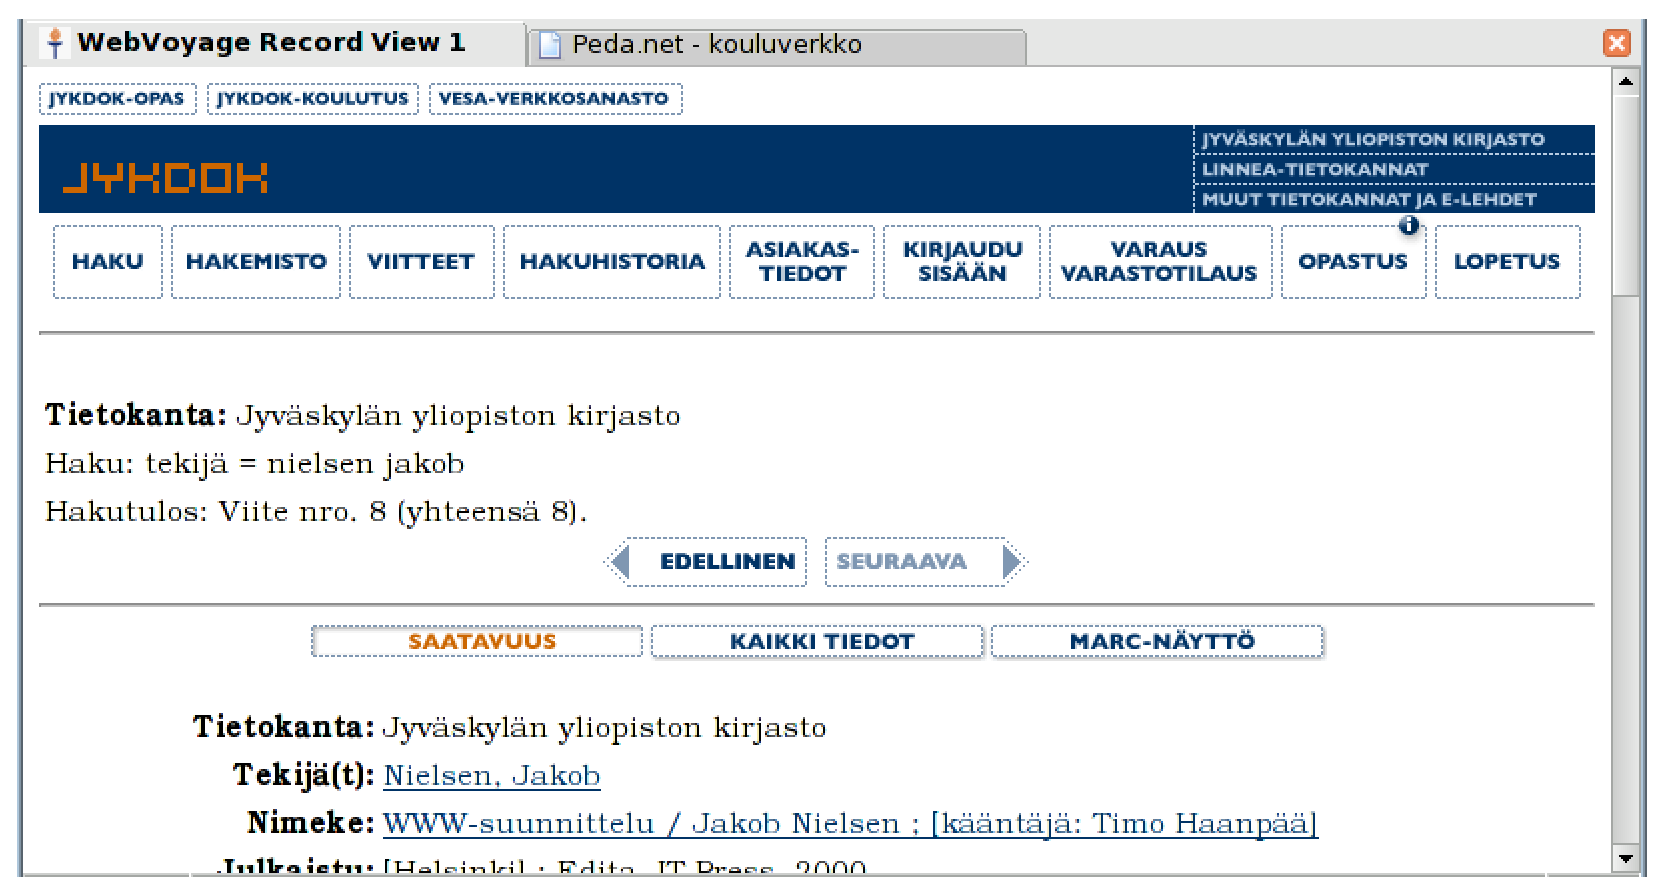
\includegraphics[width=14cm]{kuvat/kirjasto1}
\caption{Kirjaston hakupalvelun tulos}
\label{fig:kirjasto1}
\end{kuva}

Siirryn hetkeksi tarkistamaan toisessa selaimen ikkunassa, ett� t�m�
oli juuri se kirja, jota toisella sivustolla suositeltiin ja nostan
t�m�n ikkunan esiin muiden alta muutamaa minuuttia my�hemmin. Suureksi
h�mm�styksekseni juuri hakemani tiedot on hukattu, koska ``yhteytesi
tietokantaan on katkennut aikarajoituksen vuoksi'' (ks. kuva
\ref{fig:kirjasto2}). Ei minua k�ytt�j�n� kiinnosta mist� tiedot
haetaan ja erityisesti minua ei kiinnosta kuinka pitk�n yhteyden
tietokanta kerrallaan sallii. Palvelun tekij�ll� on selv�stikin ollut
ajatuksena valvoa n�in lyhyell� aikarajalla sit�, onko ikkuna viel�
aktiivisessa k�yt�ss�. Jostain syyst� on p��tetty, ett� jos k�ytt�j� ei
tee jotain muutaman minuutin sis�ll� niin silloin ``oikea'' toimenpide
on \emph{poistaa hakutulokset tai muu vastaava sis�lt�}. Sovellusta
tehdess� olisi ehk� kannattanut mietti�, olisiko sovellus mahdollista
toteuttaa siten, ett� tietokantapalvelimen aikarajan umpeutuessa
k�ytt�j�lle luovutettu sivu j�tet��n ennalleen ja huolehditaan
aikarajan umpeen menemisest� vasta, \emph{jos} k�ytt�j� viel� yritt��
tehd� jotain muuta.

\begin{kuva}
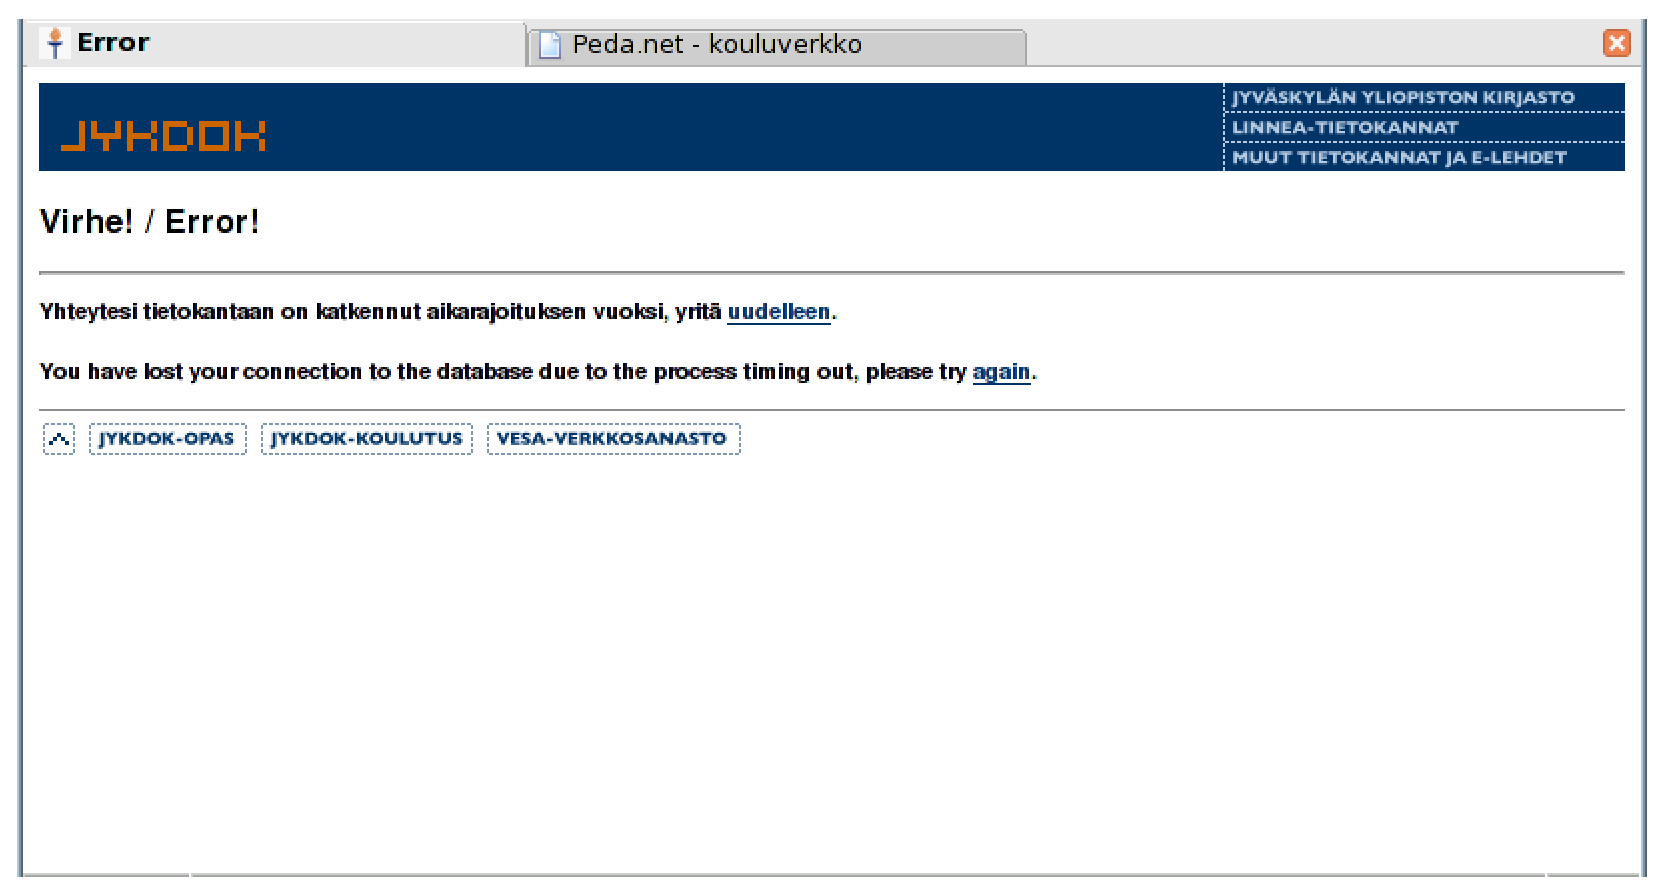
\includegraphics[width=14cm]{kuvat/kirjasto2}
\caption{Kirjaston hakupalvelun tulos kolme minuuttia haun j�lkeen}
\label{fig:kirjasto2}
\end{kuva}

\subsection{Selaink�ytt�iset ohjelmat tulee suunnitella toisin}

Tapahtumien avulla toimiva ohjelmalogiikka ei siis sin�ns� ole
syyllinen t�h�n ongelmaan, vaan se, ett� selaink�ytt�inen ohjelma ei
voi luottaa siihen, ett� kaikista asioista syntyisi tapahtuma. T�m�n
rajoituksen vuoksi sokeasti perinteisen mallin mukaisesti toteutettu
ohjelma toimii ep�vakaasti selaink�ytt�isen�.

\section{Perinteisten mallien sopimattomuus verkkoon}
\label{tiers}

Ohjelmistotuotannossa k�ytt�j�n kanssa vuorovaikutuksessa toimiva
ohjelmisto pyrit��n perinteisesti jakamaan kahteen tai kolmeen
kerrokseen. Kaksikerroksisessa mallissa (kuva \ref{fig:2tier}) ohjelman
logiikka erotetaan k�ytt�liittym�logiikasta ja kolmikerroksisessa
mallissa (kuva \ref{fig:3tier}) ohjelman logiikka jaetaan viel�
sovelluslogiikkaan ja tiedon k�sittelyn logiikkaan. Molemmissa
malleissa k�ytt�liittym� pidet��n omassa kerroksessaan erityisesti
siksi, ett� vaihtoehtoisen k�ytt�liittym�n rakentaminen olisi
mahdollisimman helppoa. K�yt�nn�ss� k�ytt�liittym�st� vastaava kerros
kutsuu melkein kaikkien toimintojen yhteydess� sovelluslogiikkaa ja
itse k�ytt�liittym�kerroksessa on kohtuullisen v�h�n ohjelmakoodia.
Voisi sanoa, ett� k�ytt�liittym�kerroksen teht�v� on tulkita
k�ytt�j�lle n�kyv�st� k�ytt�liittym�st� syntyneet tapahtumat eri
toiminnoiksi, jotka sitten edelleen ohjataan sovelluslogiikan
k�sitelt�v�ksi. T�m�n ansiosta ohjelma on yleens� helppo siirt��
esimerkiksi toimimaan jonkin toisen grafiikkakirjaston p��lle.
Kolmikerrosmallissa etuna on helppo siirrett�vyys my�s uudelle
tallennusmedialle.

\begin{kuva}
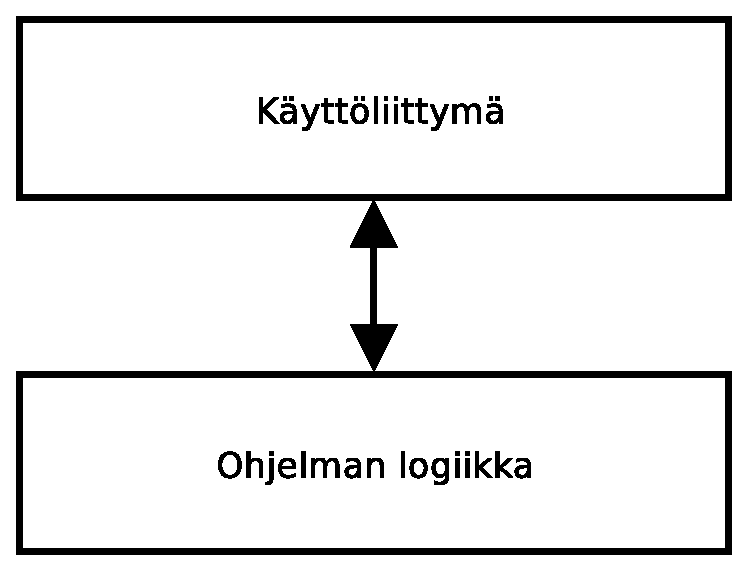
\includegraphics[width=5cm]{kuvat/fig2tier}
\caption{Kaavio kaksikerroksisesta ohjelma"-arkkitehtuurista}
\label{fig:2tier}
\end{kuva}

\begin{kuva}
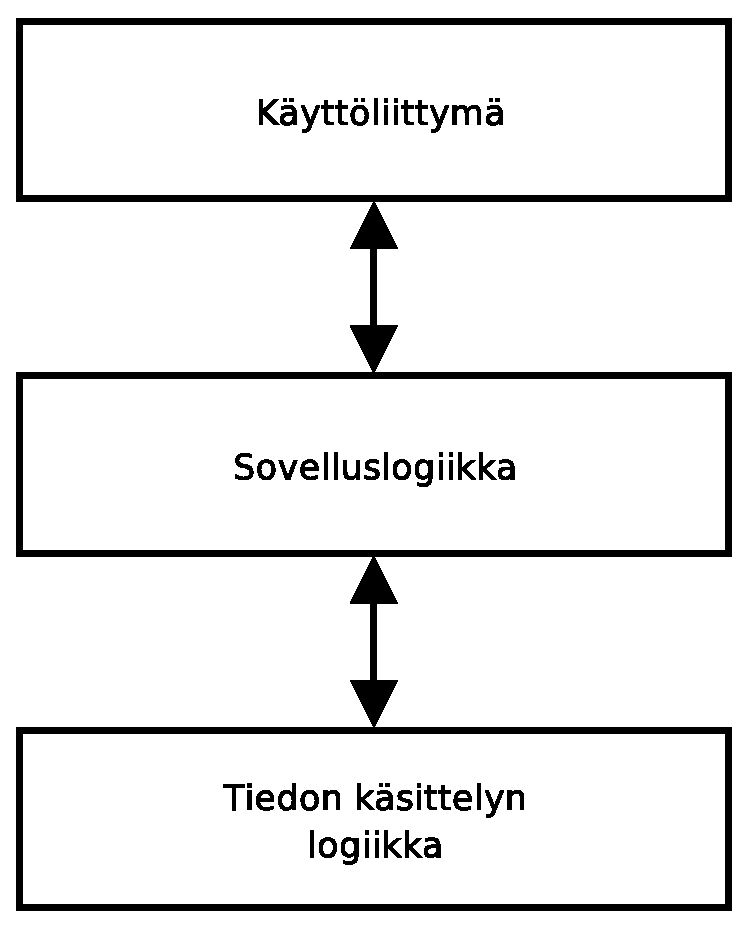
\includegraphics[width=5cm]{kuvat/fig3tier}
\caption{Kaavio kolmikerroksisesta ohjelma"-arkkitehtuurista}
\label{fig:3tier}
\end{kuva}

Verkossa toimivissa eli useinmiten selaink�ytt�isiss� ohjelmissa eteen
tulee perinteisess� mallissa kohtaamattomia ongelmia: k�ytt�liittym�n
toiminta on yhteydet�n, k�ytt�j� voi haarauttaa istunnon ja j�rjestelm�
ei voi erottaa verkon virheellist� toimintaa ja k�ytt�j�n hieman
tavallisesta poikkeavaa k�ytt�ytymist� toisistaan. Lis�ksi eri
selainohjelmien toteutuksissa on usein merkitt�vi� ohjelmavirheit�.
N�m� asiat kuuluvat k�ytt�liittym�kerrokseen, sill� ne eiv�t ole
ohjelman toimintalogiikan (eli sovelluslogiikan) kannalta olennaista
tietoa. Ongelmana vain on, ett� k�ytt�liittym�n toteutuksesta tulee
hyvin ty�l�s ja jos selaink�ytt�isi� ohjelmia tehd��n useita, joudutaan
k�ytt�liittym��n kuuluva kerros kirjoittamaan yh� uudelleen ja
uudelleen.

Teknisten ongelmien lis�ksi tulee ottaa huomioon my�s k�ytt�jien
tottumukset ja selainohjelmien p��asiallinen k�ytt�tarkoitus:
www"-sivujen selailu. Eri selainohjelmissa on erilaisia
erikoistoimintoja tavallisten sivujen selailun nopeuttamiseksi ja
tehostamiseksi. Jos selaink�ytt�ist� ohjelmaa ei voi k�ytt�� kuten
tavallisia www"-sivuja, joutuu k�ytt�j� opettelemaan j�lleen yhden
uuden ohjelman k�ytt�liittym�n ja h�n joutuu aina t�t� ohjelmaa
k�ytt�ess��n toimimaan eri tavalla kuin muilla www"-sivuilla. T�m�
lis�� k�ytt�j�n muistikuormaa ja heikent�� osaltaan sovelluksen
k�ytett�vyytt�.

\section{K�ytt�liittym�n esitt�minen verkon ehdoilla}

Verkossa toimivissa selainpohjaisissa k�ytt�liittymiss� perustavan
laatuinen ongelma on, ett� sivut tai k�ytt�liittym�n lomakkeet t�ytyy
esitt�� HTML"-kielen avulla. HTML on kuitenkin suunniteltu staattisten
dokumenttien esitt�miseen \cite{w3:html}. My�s
selaimet\footnote{HTML"-standardissa k�ytet��n sana ``selain'' sijasta
sanaa ``k�ytt�j�agentti'' korostamaan sit� seikkaa, ett� sivuja ei
v�ltt�m�tt� selailla, vaan (tietokone)agentti k�y k�ytt�j�n puolesta
lukemassa sivuja ja tekee niist� vaikkapa yhteenvetoja. Esimerkki usein
k�ytetyst� agentista voisi olla Google. My�s selain voisi olla enemm�n
kuin pelkk� selain esimerkiksi ker��m�ll� sivustosta vain linkit
normaalien sivujen n�ytt�misen sijasta.} on suunniteltu p��asiassa
staattisten sivukokonaisuuksien lukemiseen ja sen vuoksi selaimissa
onkin esimerkiksi \emph{takaisin}"-toiminto (\alt{Back}). Lis�ksi
selaimet k�ytt�v�t sivujen tiedonsiirrossa HTTP"-protokollaa, jonka
seurauksena k�ytt�liittym�t eiv�t ole koko ajan yhteydess� palvelimen
p��ss� toimivaan sovelluslogiikkaan. Perinteiset k�ytt�liittymien
suunnittelutavat ja toteutusmallit soveltuvat huonosti selaink�ytt�isen
k�ytt�liittym�n toteutukseen. Esittelen seuraavassa muutamia suurimpia
ongelmia, jotka syntyv�t pohjalla olevista arkkitehtuurieroista. Tulee
kuitenkin huomata, ett� osa ongelmista syntyy siit�, ett� kokenut
www"-selaimen k�ytt�j� odottaa \emph{enemm�n vapauksia} ohjelman
k�ytt�tavoissaan johtuen siit�, ett� tavallisten www"-sivujen
yhteydess� erilaisia k�ytt�tapoja on useita. Hyv� selaink�ytt�inen
ohjelma pystyykin vastaamaan n�ihin odotuksiin.

\section{Yhteydet�n k�ytt�liittym�}

WWW"-selaimet k�ytt�v�t tiedon siirtoon HTTP"-yhteytt� tai SSL"-salattua
HTTP"-yhteytt� (t�st� k�ytet��n usein lyhennyst� \alt{HTTPS}). Molemmat
n�ist� yhteysmalleista ovat loogisesti yhteydett�mi�, vaikka
tehokkuuden vuoksi todelliset toteutukset pit�v�tkin yhteyden usein
auki eri dokumenttien noutamisen v�lill�. Selain voi milloin tahansa
katkaista entisen yhteyden ja luoda uuden, mutta t�m� ei saa vaikuttaa
ohjelman toimintaan.

Yhteydett�m�n toiminnan vuoksi k�ytt�liittym�n toiminnot t�ytyy
suunnitella siten, ett� yhdell� lomakkeella teht�v�t toiminnot eiv�t
vaadi ohjelman sis�lt��n puuttumista ennen seuraavalle lomakkeelle
siirtymist�. Ongelma voidaan osittain kiert�� k�ytt�m�ll�
JavaScript"-skriptikielt� asiakkaan selainohjelmassa, mutta koska
verkkoymp�rist�ss� asiakasohjelmaan ei voi luottaa, t�ytyy sama
sovelluslogiikka olla my�s palvelimen
p��ss�.\footnote{JavaScript"-skriptikielell� voi esimerkiksi tarkistaa
onko sy�tekentt��n k�ytt�j�n kirjoittama tieto laskun viitenumero
laskemalla onko viitenumeron viimeinen tarkistusnumero oikein. Jos
tarkistusnumero ei toimi, n�ytet��n varoitusikkuna ja pyydet��n
k�ytt�j�� sy�tt�m��n tieto uudelleen. Kuitenkin, turvallisuussyist�
sama tarkistus t�ytyy tehd� my�s palvelimella (koska muuten
pahantahtoinen asiakas voisi muuttaa selaimessa toimivaa
JavaScript"-ohjelmaa ja l�hett�� virheellisen numeron j�rjestelm��n).}
T�st� seuraa, ett� sama toiminnallisuus t�ytyy esitt�� kahdella eri
ohjelmointikielell� (JavaScript ja kieli, jolla palvelimen logiikka on
tehty). Seurauksena on koko j�rjestelm�n huomattavasti vaikeampi
yll�pito, koska eri kielill� tehtyjen toimintojen t�ytyy vastata
toisiaan. Vaihtoehtona on my�s toteuttaa kevyt tarkistus selaimen
p��ss�, jossa pyrit��n karsimaan suurimmat virheet pois, mutta sy�tetyn
tiedon oikeellisuus t�ytyy edelleen tarkistaa my�s palvelimen p��ss�.
Lis�ksi tulee huomata, ett� jos osa toiminnoista \emph{vaatii}
JavaScript"-kielen tukea, ei sovellus en�� toimi mill� tahansa
www"-selaimella.

\section{Ongelmallinen takaisin"-painike}

Kuten edell� mainitsin, selaimet on suunniteltu staattisten
dokumenttien k�ytt�miseen. Lis�ksi HTTP"-protokollan m��ritys erikseen
huomauttaa, ett� asiakasohjelman historiatietojen k�yt�n ei tarvitse
hakea tietoja palvelimelta \cite[kappale 13.13]{ietf:http}.
Esimerkkitapaus ongelmatilanteesta on esitetty kuvassa \ref{fig:fork}.
Esimerkiss� k�ytt�j� siirtyy ensin sovelluslogiikan luomalle sivulle
(lomakkeelle) $A$, valitsee toiminnon $a_1$ ja siirtyy sen seurauksena
sivulle $B$. T�m�n j�lkeen k�ytt�j� voi k�ytt�� selaimen
\emph{takaisin}"-toimintoa ja palata takaisin sivulle $A$. Koska t�m� on
siirtyminen selainohjelman historiatiedoissa, ei asiasta protokollan
mukaisesti tarvitse ilmoittaa palvelimelle, joten sovelluslogiikan
n�k�kulmasta asiakas on edelleen sivulla $B$. T�m�n j�lkeen asiakas
valitsee edellisest� poikkeavan toiminnon $a_2$. Palvelinohjelman tulee
t�ss� vaiheessa kyet� huomaamaan, ett� vaikka sen tarjoama lomake
olikin $B$, on k�ytt�j�n valitsema toiminto $a_2$ ja toimintoon
liittyv� tieto on per�isin lomakkeelta $A$, eik� lomakkeelta $B$.

Usein t�h�n ongelmaan k�ytetty ``ratkaisu'' on kertoa k�ytt�j�lle, ett�
sovelluksessa \emph{ei saa} k�ytt��
\emph{takaisin}"-toimintoa.\footnote{T�m� rajoitus seuraa yleens� siit�,
sovellus yritt�� pit�� istunnon tilaa yll�. Usein t�h�n k�ytet��n
keksej� (\alt{cookies}). N�iden suurin ongelma on, ett� niihink��n ei
voida helposti vaikuttaa historiatoimintojen yhteydess� ja lis�ksi ne
ovat globaaleja kaikkien selainohjelman ikkunoiden kesken. Jos istuntoa
kuvaavassa keksiss� s�ilytet��n my�s k�ytt�j�n tunnistetietoja ei
sovellukseen voi kirjautua monella eri k�ytt�j�tunnuksella
samanaikaisesti -- paitsi jos k�ytt�� eri selainohjelmaa jokaista
k�ytt�j�� kohden.} Olennaista on kuitenkin huomata, ett� k�ytt�j� teki
tietoisen p��t�ksen k�ytt�ess��n -- tai yritt�ess��n k�ytt�� --
kyseist� toimintoa ja varmastikin h�n olisi halunnut sen tekev�n jotain
muuta, kuin n�ytt�v�n virheilmoituksen.

%Ohjelma tulee siis tehd� sellaiseksi, ett� se pystyy vastaanottamaan ja k�sittelem��n \emph{mahdollisimman suuren} osan k�ytt�j�n l�hett�m�st� tiedosta, vaikka muuttuneen tilanteen vuoksi osa siit� ei olisikaan relevanttia.

\section{Istunnon haarautuminen}

Istunnon haarautuminen liittyy hyvin l�heisesti
\emph{takaisin}"-toimintoon. Siin� erona, k�ytt�j� kahdentaa aktiivisen
lomakkeen $A$ ja valitsee ensimm�isess� ikkunassa toiminnon $a_3$ ja
toisessa ikkunassa toiminnon $a_4$. J�rjestelm� palauttaa toiminnon
$a_3$ seurauksena sivun $C$ ja toiminnon $a_4$ seurauksena sivun $D$.
J�rjestelm�n kannalta t�m� tapahtuma n�ytt�� t�sm�lleen samalta kuin
\emph{takaisin}"-toiminnon k�ytt�kin, mutta merkitt�v� ero syntyy siit�,
ett� seuraavaksi k�ytt�j� voi tuottaa rinnakkaisia tapahtumia sek�
lomakkeelle $C$, ett� lomakkeelle $D$. Ei siis riit�, ett�
palvelinohjelma pit�� kirjaa k�ytt�j�n toimintahistoriasta ja osaa
peruuttaa l�hetettyjen kutsujen mukaan oikeaan tilanteeseen; lis�ksi
ohjelman pit�� kyet� haarauttamaan istuntoja ep�suorien tapahtumien
kautta. T�ysin oikean istuntoa kuvaavan tiedon yll�pit�minen
palvelimella onkin v�hint��nkin hyvin ty�l�st� ellei mahdotonta.
Istunnon tiedot t�ytyy siis jotenkin saada siirtym��n selainohjelmassa
ikkunakohtaisesti, jolloin ikkunan kahdentaminen kahdentaa my�s
istunnon.

\begin{figure}[htb]
\begin{center}
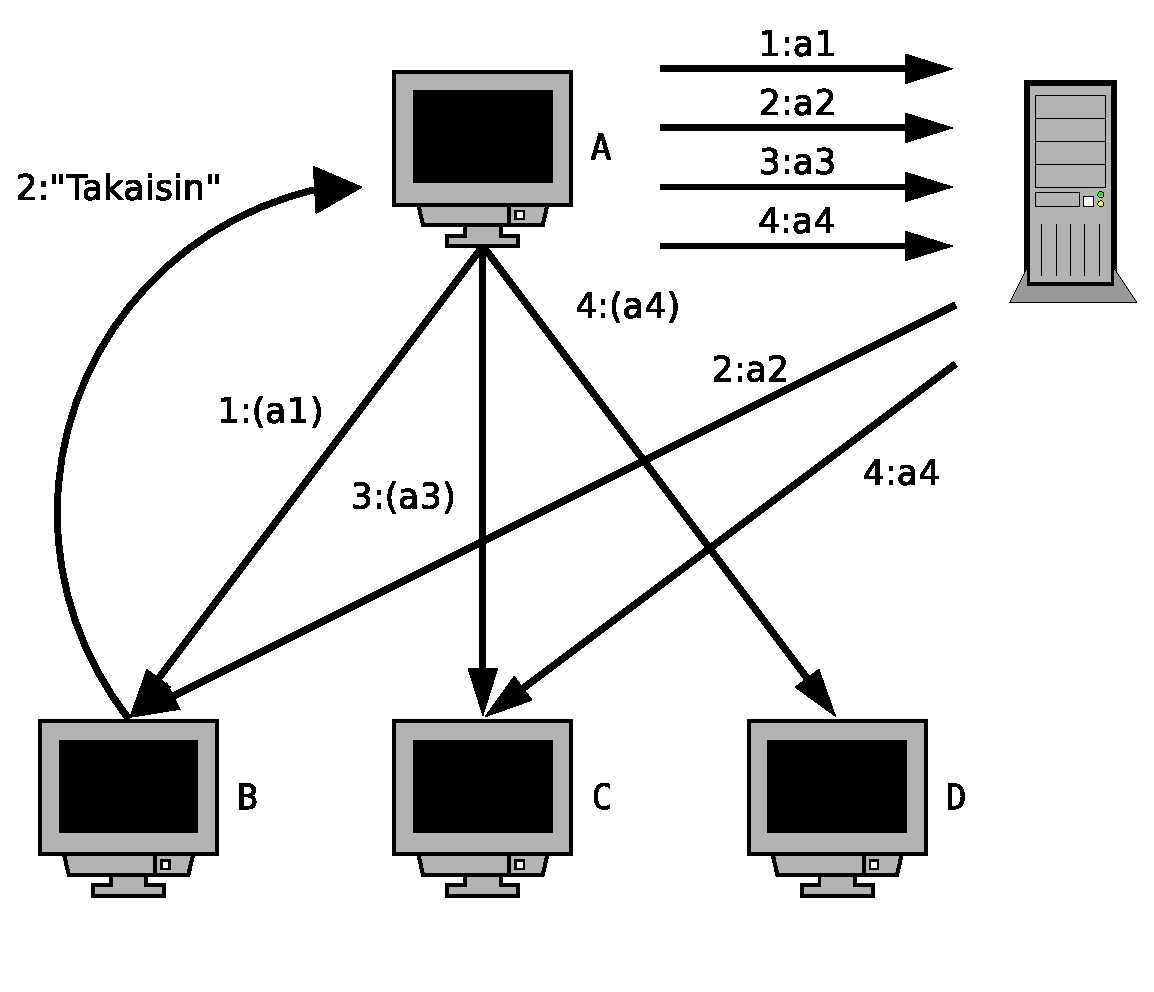
\includegraphics[width=10cm]{kuvat/fork}
\caption{Kaavio istunnon haarautumisesta}
\label{fig:fork}
\end{center}
\end{figure}

\section{Selaimen historia"-toiminnot}

Todellisuudessa takaisin"-painike ja uusien ikkunoiden avaaminen on vain
pieni osa itse varsinaista ongelmaa. Selaimet pit�v�t kirjaa kaikista
vierailluista sivuista ja koska selaink�ytt�isten sovellusten t�ytyy
esitt�� k�ytt�liittym�ns� HTML"-sivuina, kirjautuvat my�s t�llaisen
sovelluksen kaikki n�yt�t historia"-tietoihin. Sivuhistorian kautta
k�vij� voi palata \emph{suoraan mille tahansa sivulle} milloin tahansa.
Ei siis riit�, ett� varaudutaan siihen, ett� k�ytt�j� voi palata
edelliselle sivulle takaisin"-painikkeella, vaan kaikkien aikaisemmin
n�ytettyjen sivujen t�ytyy toimia.

Historiatoimintojen vuoksi ainoastaan takaisin"-painikkeen testaaminen
ei riit� testausvaiheessa. T�m�n seurauksena pelk�st��n takaisin- ja
eteenp�in "-painikkeiden testaaminen j�rjestelm�llisell� menetelm�ll�
\cite{lucca:web_application_testing} ei ole riitt�v�
testimenetelm� ohjelman oikean toiminnan varmistamiseksi.

K�yt�nn�ss� t�m� tarkoittaa sit�, ett� palvelimen p��ss� ei kannata
yritt�� pit�� kirjaa siit�, mik� n�kym� k�ytt�j�lle on annettu ja
erityisesti ei tule arvata, mik� n�kym� k�vij�n selaimessa on
aktiivinen.

\section{Verkon virheiden havaitseminen on mahdotonta}

Yhteydett�m�st� k�ytt�liittym�st� seuraa my�s, ett� palvelin ei voi
tunnistaa tietoverkon virheellist� toimintaa esimerkiksi asiakkaan
selaimen sulkemisesta tai asiakkaan tietokoneen jumiutumisesta.
Yll�mainitut ongelmatilanteet  n�kyv�t palveliohjelmalle t�ysin samalla
tavalla kuin, jos asiakas vain k�ytt�isi ep�tavallisen kauan aikaa
lomakkeen t�ytt�miseen. T�m�n vuoksi mik��n toiminto ei saisi lukittaa
resursseja siihen asti kunnes ``k�ytt�j�n istunto loppuu''. K�yt�nn�ss�
t�llaisia resurssien lukittamisia kuitenkin tarvitaan ja usein
ratkaisuna on k�ytt�� maksimiaikaa lukitukselle; kun k�ytt�j� valitsee
esimerkiksi uutisartikkelin muokattavaksi, merkit��n muokattava
artikkeli lukituksi, jolloin muut eiv�t voi sit� muokata. Lukitus
puretaan kun k�ytt�j� tallentaa muokatun artikkelin tai kun
ennaltam��r�tty maksimiaika lukitukselle on kulunut. T�ss�kin on
tietenkin ongelmana, ett� ongelmatilanteissa lukittu resurssi on
k�ytt�kelvoton valittuun aikarajaan asti. Parempi vaihtoehto olisikin
sallia rinnakkaisten muutosten tekeminen esimerkiksi versionhallinnan avustamana.

\section{Selainten virheelliset toteutukset}

Kun palvelimen ohjelmisto on saatu toimimaan ja kaikki edell�mainitut
ongelmat on otettu huomioon, havaitaan, ett� eri selainohjelmat eiv�t
toimi eri standardeissa m��r�tyll� tavalla. Useimmat vioista
vaikuttavat ainoastaan k�ytt�j�lle n�kyv�n lomakkeen ulkoasuun --
esimerkiksi joku teksti on suhteessa muuhun k�ytt�liittym��n
suuremmalla tekstill� kuin pit�isi. Kuitenkin osa vioista voi est��
tiettyjen toimintojen k�yt�n: esimerkiksi HTML"-m��rityksen mukaan
yhden \code{file}"-tyyppisen lomake"-elementin tulee tarjota
mahdollisuus usean tiedoston siirt�miseen yht� aikaa. Ainoa yleisesti
k�yt�ss� oleva selain, joka toimii t�ss� mieless� m��rityksen
mukaisesti, on Opera. T�m� n�kyy my�s yleisimmiss� palvelinp��n
toteutuksissa siten, ett� Operalla monta tiedostoa yht� aikaa
l�hetett�ess�, tapahtuu palvelinp��ss� yleens� virhe tiedostoja
vastaanotettaessa, koska palvelinohjelmiston kehitt�j� ei ole lukenut
m��rityst� vaan ainoastaan tarkkaillut kuinka yleisimm�t selaimet
toimivat. \cite{korpela:file_input}

Toinen yleinen virhe selainten toteutuksessa on tiedon l�hett�minen
UTF-8"-koodauksella ilman siit� ilmoittamista -- protokollan mukaan
oletuksena tulee t�ll�in k�ytt�� ISO-8859-1"-merkist��, jonka
seurauksena kaikki ASCII"-merkist�n ulkopuoliset merkit siirret��n
v��rin. T�ss� siis puutteellisen toiminnan lis�ksi tuhoutuu my�s
tietoa. T�m� ongelma voidaan kiert�� esimerkiksi l�hett�m�ll�
lomakkeella n�kym�t�n kentt�, jonka sis�lt� on tunnettu ja sis�lt��
ASCII"-merkist�n ulkopuolisia merkkej�, ja tarkastelemalla kuinka
selain koodaa t�m�n kent�n sis�ll�n.


\chapter{Er�s ratkaisumalli selaink�ytt�liittym�n toteutukseen}

\begin{chapterquote}{Keskustelu Matrix-elokuvassa}
Neo: "You mean I can dodge bullets?"\\
Morpheus: "I mean when you are ready, you won't have to."
\end{chapterquote}

Kuten luvussa \ref{ongelmia} kuvasin, selaink�ytt�isten ohjelmien
k�ytt�liittymien toteuttamisessa on useita ongelmia. Kuvailen t�ss�
luvussa ratkaisuvaihtoehtoja tuossa luvussa kuvattujen ongelmien
ratkaisemiseksi. Osa suunnittelemistani ratkaisuvaihtoehdoista
osoittautui ep�k�yt�nn�llisiksi, mutta kuvailen ne siit� huolimatta
antamaan kuvaa ratkaisujen kehityskaaresta.

\section{K�ytt�liittym�kerroksen jakaminen osiin}

Ensimm�isen� ajatuksena oli jakaa luvussa \ref{tiers} kuvattu
kolmikerroksinen malli viel� kerran, p��tyen nelikerroksiseen
rakenteeseen. T�ss� mallissa k�ytt�liittym�kerros jaetaan
k�ytt�liittym�n toiminnallisuuden kuvaamiseen ja k�ytt�liittym�ajuriin
(kuva \ref{fig:4tier}).

\begin{figure}[htb]
\begin{center}
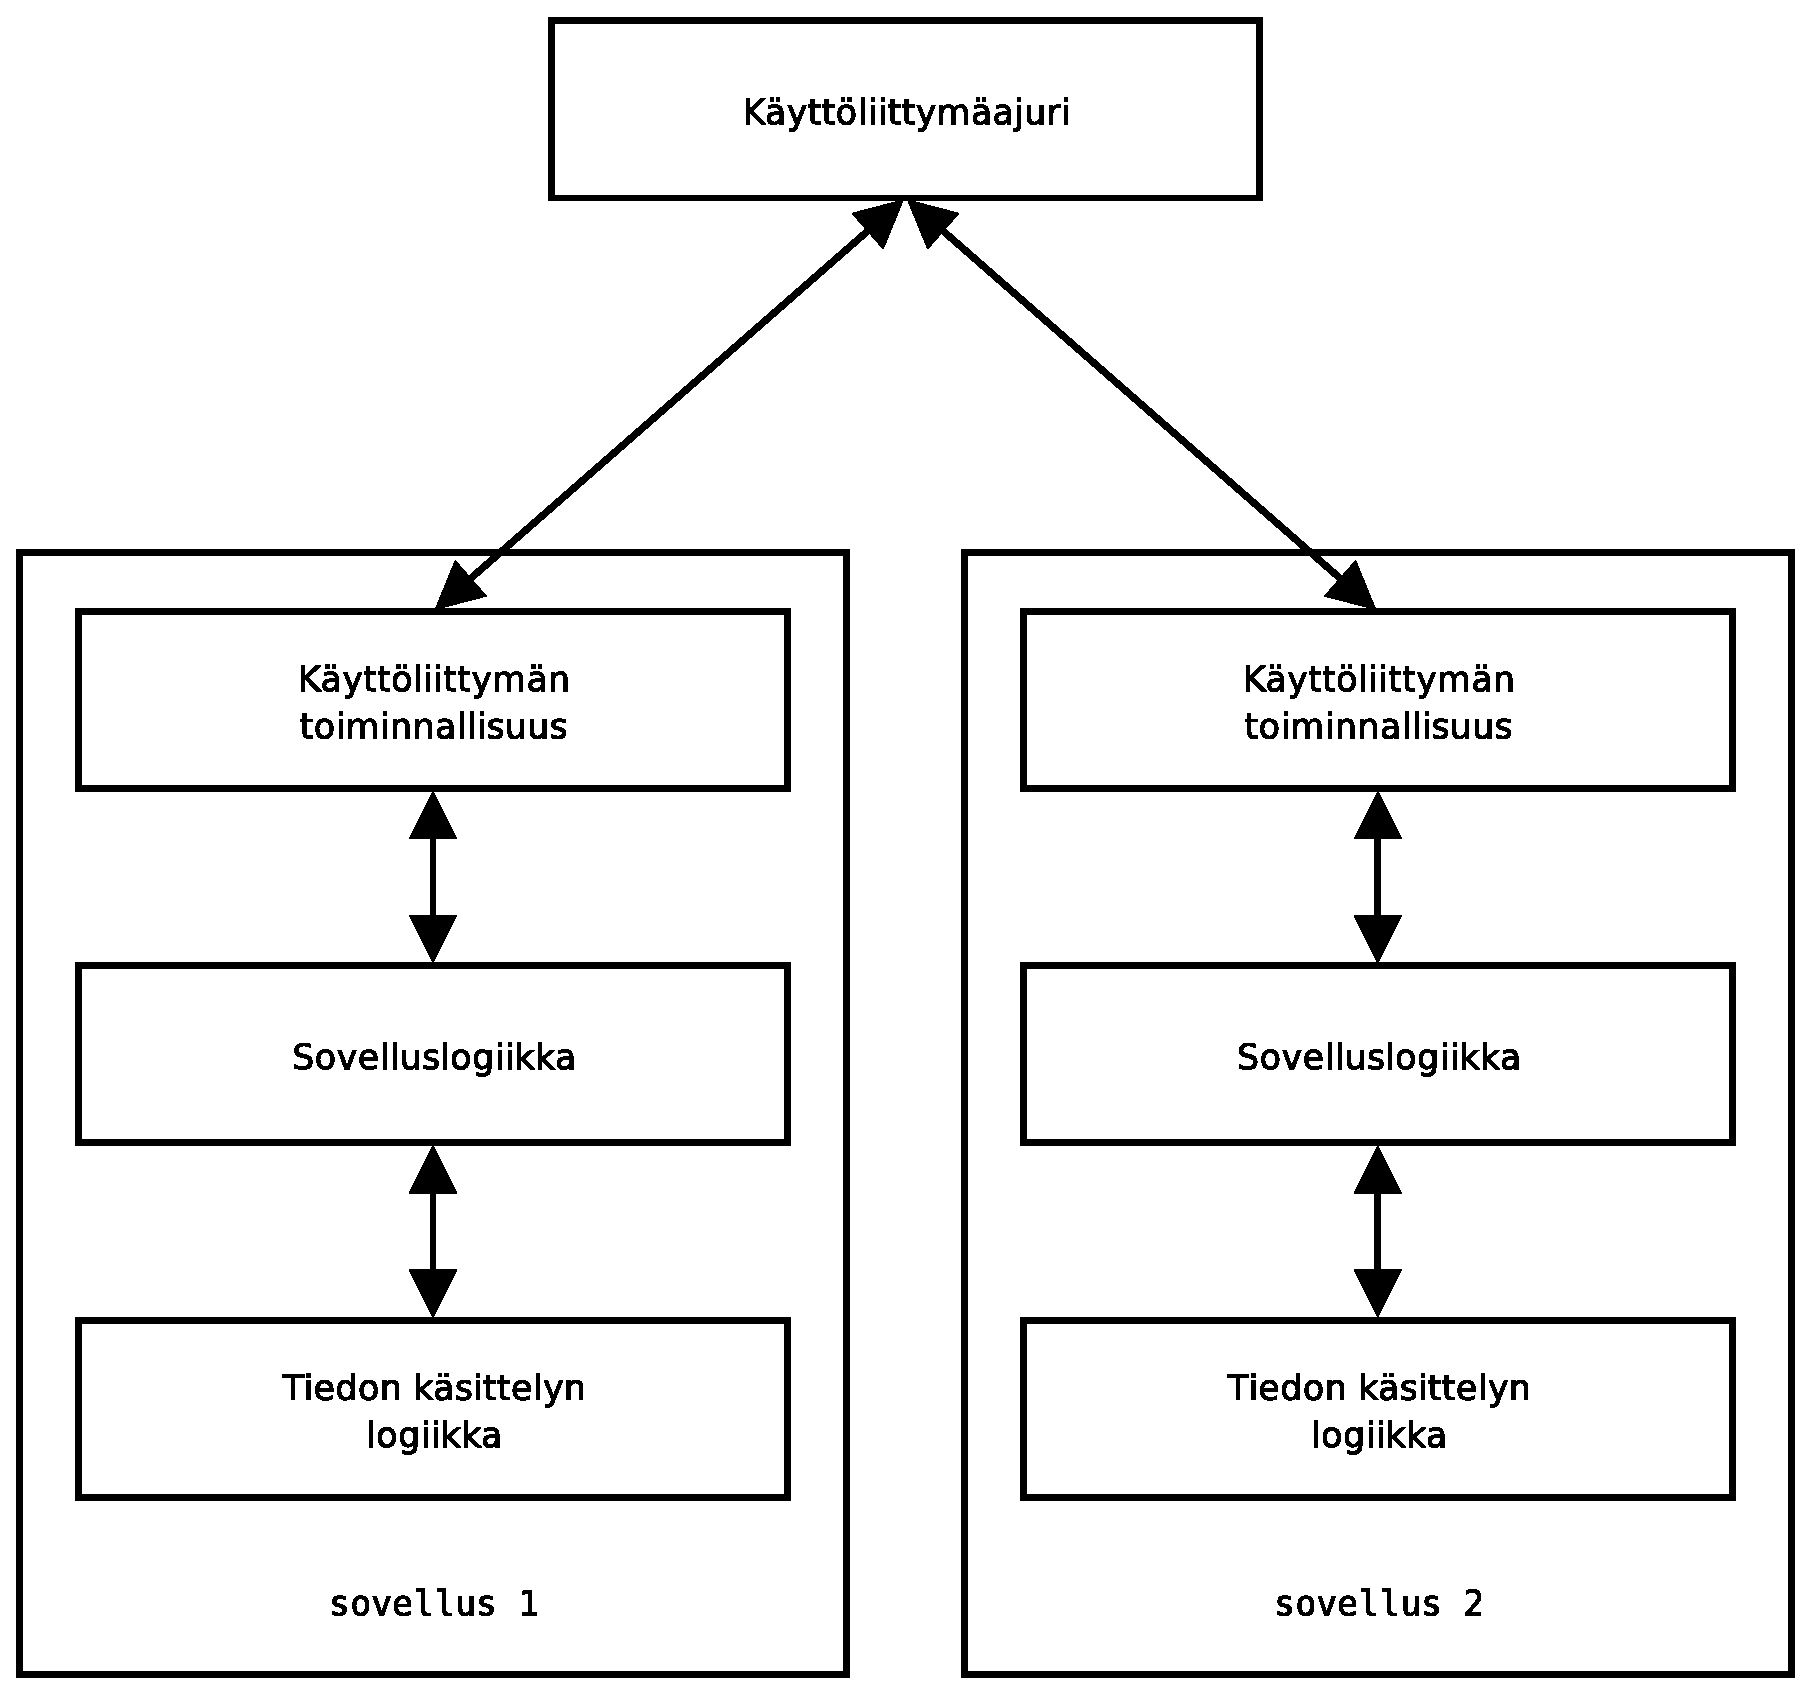
\includegraphics[width=10cm]{kuvat/fig4tier}
\caption{Kaavio nelikerroksista arkkitehtuurista usean sovelluksen tapauksessa}
\label{fig:4tier}
\end{center}
\end{figure}

Jaon etuna eri sovellusten k�ytt�liittym�t saadaan toimimaan
vastaavalla ulkon��ll� ja mahdollisimman pitk�lti vastaavilla
toiminnoilla. T�m� onnistuu jakamalla k�ytt�liittym�ajuri eri
sovellusten kesken. Suunnittelemalla k�ytt�liittym�n toiminnallisuuden
ja k�ytt�liittym�ajurin rajapinta sopivasti, helpottuu k�ytt�liittym�n
kirjoittaminen verrattuna entiseen malliin, jossa k�ytt�liittym��
kirjoitettaessa jouduttiin kirjoittamaan koodi my�s k�ytt�liittym�n eri
osien, kuten erilaisten painikkeiden, hallintaan. Uudessa mallissa
k�ytt�liittym�n kuvauksessa vain ilmoitetaan, ett� k�ytt�j�n tulee
valita annetusta listasta kaksi tai kolme kohtaa. K�ytt�liittym�ajuri
voisi sitten toteuttaa tuon esityksen esimerkiksi ryhm�ll� \alt{radio
button} -tyyppisi� grafiikkaelementtej� tai vaihtoehtoisesti
valintalaatikon (\alt{select box}) avulla. WWW-k�yt�ss�
k�ytt�liittym�ajurin muodostamaa lopputulosta voitaisiin viel� hioa
kirjoittamalla lomakekohtaisia ulkon�k�asetuksia CSS-kielell�
\cite{w3:css}.

K�ytt�liittym�ajuri keskustelee www-selaimen kanssa, mutta
vaihtoehtoisesti sen voisi toteuttaa natiivilla sovelluksella. T�ll�in
edes ohjelman k�ytt�liittym�n kuvausta ei tarvitsisi muuttaa vaikka
k�ytt�ymp�rist� vaihtuisi selaink�ytt�isest� natiiviksi. Koska
toiminnallisuuden t�ytyy kuitenkin olla lomakepohjainen toimiakseen
\emph{hyvin} selaimen kautta, ei t�llainen natiivik�ytt�liittym� olisi
merkitt�v�sti parempi kuin selainpohjainen k�ytt�liittym�k��n.
V�it�nkin, ett� selaink�ytt�isten ohjelmien k�ytt�liittymien logiikka
ja dialogien rakenne pit��kin suunnitella eri tavalla kuin
perinteisten, k�ytt�j�rjestelm�n omien s��nt�jen mukaan toimivien
sovellusten.

\subsection{Tiedon k�sittelyn logiikka}

T�m� kerros toteutetaan k�ytt�m�ll� jotain olemassaolevaa tietokantaa,
esimerkiksi MySQL tai PostgreSQL. Teoriassa tietokannan pit�isi
ymm�rt�� ja valvoa kaikki tiedon esitysmalliin liittyv�t rajoitukset,
mutta koska tietokantoja k�sitell��n k�yt�nn�ss� aina SQL-kielen
avulla, ei riippuvuustietoja voida kattavasti esitt��
tietokantavalmistajasta riippumattomalla tavalla. Jos ohjelmasta
halutaan siirrett�v�, jolloin sit� voidaan k�ytt�� monen eri
tietokantaohjelmiston kanssa, t�ytyy melkein kaikki tarkistukset tehd�
sovelluslogiikassa. Tietokannan tehokkuus voidaan maksimoida
ohjelmoimalla tarkistukset ja rajoitukset tietokannan omilla
ty�kaluilla, mutta siirrett�vyys menetet��n. Pyrin itse pit�m��n
selaink�ytt�iset sovellukset tietokantariippumattomina, koska olen
kokenut, ett� k�yt�nn�ss� eri tietokannan k�ytt�misest� saatava
nopeusero on suurempi kuin yksitt�isen tietokannan hienos��t�misest�
saatava nopeusero. Eli pitk�ll� aikav�lill� suurin nopeuden
kasvattaminen saataisiin aikaiseksi vaihtamalla tietokantaa aina sen
hetkisen sis�ll�n ja k�ytt�profiilin mukaisesti nopeiten toimivaan.
Koska tietokantasovelluksissakin on virheit�, ei t�llaisesta
tietokannasta toiseen siirtymist� voi kuitenkaan kovin usein
suositella. T�m�n tutkielman kannalta tarkka jako ei ole olennaista.

\subsection{Sovelluslogiikka}

Sovelluslogiikka vastaa sovelluksen ``�lyst�''. Teoriassa t�ss�
kerroksessa ei oteta mit��n kantaa sovelluksen k�ytt�liittym��n.
K�yt�nn�ss� t�m� kerros on todenn�k�isesti tehokkainta sulauttaa
osittain k�ytt�liittym�n toiminnallisuuden kanssa. N�in sen vuoksi,
ett� sovelluslogiikkaan ei yleens� ohjelmoida ominaisuuksia, joita
k�ytt�liittym�n toiminnallisuus ei tarvitse. Toisaalta k�ytt�liittym��n
ei voida lis�t� ominaisuuksia, joita sovelluslogiikka ei voi tukea. Eli
kaikki muutokset t�ytyy kuitenkin tehd� molempiin osiin! Lis�ksi
sulauttamisen haittojen voi nelj�n kerroksen mallissa olettaa olevan
kohtuullisen pieni�, koska k�ytt�liittym�n toiminnallisuus ei ole en��
niin tiukasti sidottu itse k�ytt�liittym�n ulkon�k��n.

\subsection{K�ytt�liittym�n toiminnallisuus}

K�ytt�liittym�n toiminnallisuudesta vastaava kerros kuvaa
k�ytt�liittym�n toiminnan abstraktilla tavalla: ``t�st� taulukosta
t�ytyy valita 2-5 rivi�'' tai ``k�ytt�j�n tulee sy�tt�� lomakkeelle
kaksi merkkijonoa. N�iden merkkijonojen nimet ja tyypit ovat
'k�ytt�j�tunnus':merkkijono ja 'salasana':salattu merkkijono.'' T�m�
kerros ei ota kantaa siihen miss� j�rjestyksess� taulukon sarakkeet ja
rivit n�ytet��n tai siihen, sy�tet��nk� k�ytt�j�tunnus tekstikentt��n
vai napauttelemalla hiirell� jonkin kuvan eri kohtia.

Teoriassa t�m� kerros voisi generoida yksinkertaisen XML-sivun, joka
muutettaisiin XHTML tai HTML -sivuksi selaimen toimintoja varten.
T�ll�in k�ytt�liittym�ajurin voisi kirjoittaa esimerkiksi
XSLT-kielell�. K�yt�nn�ss� t�llaisen ajurin kirjoittaminen muodostuu
oletettavasti niin hankalaksi, ett� paremmalta vaihtoehdolta tuntuu
kirjoittaa k�ytt�liittym�ajuri kirjastoksi, joka
linkitet��n\footnote{Joissakin ohjelmointiymp�rist�iss� ohjelmakoodi
k��nnet��n objektitiedostoiksi, jotka yhdistet��n \emph{linkitt�m�ll�}
valmiin ohjelman tuottamiseksi. Vasta n�in tuotettu valmis ohjelma
voidaan suorittaa. Toisaalta, esimerkiksi PHP-kielisiss� ohjelmissa
manuaalinen linkitys ei ole tarpeen, sill� se suoritetaan
automaattisesti ohjelman k�ynnistyess�.} ohjelmaan sit� teht�ess�.
Linkitys pit�� tehd� uudelleen kirjaston p�ivityksen yhteydess�, mutta
itse k�ytt�liittym�n toiminnallisuuteen ei tarvitse puuttua. T�ss�kin
mallissa eri sovellusten k�ytt�liittym�t saadaan s�ilym��n
yhdenmukaisina pelk�st��n linkitt�m�ll� kaikki sovellukset uudelleen
aina k�ytt�liittym�ajurin p�ivityksen j�lkeen.
\cite{w3:xml_v1_0,w3:xhtml,w3:xslt}

\subsection{K�ytt�liittym�ajuri}

T�m� kerros vastaa siit� kuinka k�ytt�j� pystyy tekem��n eri valinnat
ja toiminnot. Jos, k�ytt�liittym�ss� on kuvattu, ett� lomakkeella on 10
vaihtoehtoa, joista pit�� valita t�sm�lleen yksi, niin t�ll�in
selaink�ytt�isen sovelluksen k�ytt�liittym�ajuri voi n�ytt�� sivulla 10
linkki�, joista k�ytt�j� painaa yht�. Vaihtoehtoisesti ajuri voisi
n�ytt�� lomakkeen jossa on 10 \alt{radio button} -tyyppist� elementti�
ja OK-painike. Kolmas vaihtoehto olisi n�ytt��
\alt{combobox}-alasvetovalikko yhdistettyn� JavaScript-k�sittelij��n,
joka l�hett�isi lomakkeen v�litt�m�sti k�ytt�j�n n�p�ytetty� jotain
kohtaa. Optimaalisessa tapauksessa k�ytt�liittym�ajuri osaisi k�ytt��
kaikkia n�it� vaihtoehtoja ja k�ytt�j� voisi omissa asetuksissaan
valita mill� tyylill� h�n haluaa k�ytt�� erityyppisi� lomakkeita.

Koska selaink�ytt�isen sovelluksen k�ytt�j� voi haarauttaa istunnon ja
t�st� toiminnosta ei synny tapahtumaa palvelimelle, t�ytyy kaikki tieto
kuljettaa lomakkeen muun tiedon yhteydess�. T�ll�in tieto kahdentuu
automaattisesti kun k�ytt�j� kahdentaa istunnon (avaa uuden ikkunan,
jossa on sama sovellus toiminnassa) ja \emph{takaisin}-toiminnon
yhteydess� selain k�ytt�� automaattisesti entisen lomakkeen tietoja,
sill� nuo tiedot sis�ltyy siihen sivuun, jota selain k�ytt�� sivun
n�ytt�miseen. K�ytt�liittym�ajuri ei voi est�� vanhentuneen tiedon
saapumista\footnote{K�ytt�j� voisi esimerkiksi muokata
selaink�ytt�liittym�ll� uutisartikkelia, poistaa artikkelin ja k�ytt��
\emph{takaisin} toimintoa ja palata takaisin muokkaukseen. Kun k�ytt�j�
nyt tallentaa tehdyt muokkaukset t�ytyy sovelluksen joko palauttaa
poistettu artikkeli tai luoda l�hetettyjen tietojen perusteella uusi
tai k�ytt�j�n l�hett�m�� tieto hukkuu.}, joten k�ytt�liittym�n
toiminnallisuuden tai sovelluslogiikan t�ytyy ottaa siihen kantaa.
Lis�ksi istunnon koon t�ytyy olla pieni, koska sovelluksen generoimien
sivujen sis�lt�mien linkkien t�ytyy my�s sis�lt�� istunnon
tiedot\footnote{WWW-sivulla olevat linkit k�ytt�v�t aina GET-metodia
HTTP-yhteyksi� k�ytett�ess�, jossa kaikki linkin parametrit pit��
siirt�� tekstin� osoitteen lopussa. Istuntoon liittyv�t tiedot t�ytyy
siis toistaa sivun \emph{jokaisen} linkin lopussa ja sivu kasvaa
huomattavan nopeasti linkkien lukum��r�n mukaan jos istunto-tietoa on
paljon.}. HTTP-protokolla m��rittelee tavallisten linkkien k�ytt�m�n
GET-toiminnon maksimidatam��r�ksi 4 kilotavua ja lis�ksi suuri istunto
kasvattaa jokaista sivua, sill� osa istuntotiedosta joudutaan
toistamaan jokaisen linkin yhteydess�. \cite{ietf:http}

Koska \emph{kaikkien} sovellusten tietojen l�hett�minen jokaisen
lomakkeen yhteydess� vaatisi huomattavan lis�n tarvittavaan
tiedonsiirtokaistaan, tulee ohjelman toteutuksessa erikseen jakaa
istunto-tiedot kahteen osaan: lomakkeiden kautta siirtyv� tieto, ja
tieto joka voidaan jakaa my�s haarautettujen tai vanhentuneiden
tapahtumien kanssa. T�ll�in jaettu tieto voidaan s�ilytt��
palvelimella. T�llaista jaettua tietoa olisivat esimerkiksi k�ytt�j�n
henkil�kohtaiset asetukset, jotka voidaan jakaa eri ikkunoiden kesken.
Esimerkiksi valittu sivuston tyyli tai p�iv�m��rien esitysmuoto olisi
t�llaista tietoa. Istuntotietoa olisi taas esimerkiksi tieto siit�,
mit� toimintoja k�ytt�j� k�ytti saapuessaan nykyiseen n�kym��n, jos
t�t� tietoa tarvitaan tulevaisuudessa.

Tulevaisuudessa selaink�ytt�isen sovelluksen k�ytt�liittym�ajuri voisi
tuottaa XForms-m��rityksen mukaisia lomakkeita, jolloin k�ytt�liittym�n
toiminnallisuus ja ulkon�k� voidaan pit�� erill��n www-selaimeen asti.
Ik�v� kyll� XForms on hyvin heikosti tuettu nykyisiss�kin selaimissa ja
mik��n ei viittaa siihen, ett� tilanteeseen olisi tulossa nopeasti
muutosta. \cite{korpela:html_forms,w3:xforms}

\subsection{Huomioita k�ytt�liittym�ajurin toteuttamiseen liittyen}

K�ytt�liittym�ajurin t�ytyy yritt�� tunnistaa asiakasohjelma
(selaintyyppi ja versio) ja kiert�� jollakin tavalla siin� tunnetut
ongelmat. Viallisten selainten tukeen kuluva ty�aika on helpompi
perustella, koska ajuri on yhteinen monelle eri sovellukselle, joten
kustannukset ohjelmaa kohden ovat pienempi� kuin perinteisell�
mallilla.

Koska k�ytt�liittym�ajurin t�ytyy huolehtia kaikista selaimen k�yt�st�
johtuvista ongelmista, on sen toteuttaminen vaikeaa. HTML-kielt�
tukevan ajurin ei kuitenkaan tarvitse ottaa kantaa k�ytt�liittym�n
yksityiskohtiin, ainoastaan eri komponenttien j�rjestykseen, sill�
ulkon��lliset yksityiskohdat voidaan k�sitell� asiakkaan ohjelmassa
CSS-kielen avulla \cite{w3:css}. Sovellukselle voidaan helposti tuottaa
erilaisia ulkoasuja (\alt{skins}) pelk�st��n luomalla erilaisia
CSS-tiedostoja.

\section{Nelikerroksisen mallin k�yt�nn�n ongelmia}

Aloin toteuttamaan k�ytt�liittym�ajuriajatusta Peda.net-hankkeessa
teht�v�n Vihko-nimisen ty�kalun
valmistuksessa\footnote{Vihko-ty�kalusta kerrotaan tarkemmin luvussa
\ref{pedanet-vihko}}. Peda.net-hankkeessa on p��tetty yhdenmukaistaa
sovellusten toimintaymp�rist�ksi Apache/PHP-ohjelmointiymp�rist� ja
MySQL-tietokanta, joten t�m� asetti k�yt�nn�n rajoituksia ohjelman
loogiseen rakenteeseen; nykyisin k�yt�ss� oleva PHP-kielen versio 4 ei
tue moniperint�� eik� rajapintaluokkia, joten luokkahierarkian
toteuttaminen vaati liev�� luovuutta ja teoriittisesta mallista
poikkeamista.

Kuvassa \ref{fig:vihko-schema-orig} on esitetty osa alkuper�isest�
luokkahierarkiasta. Kuvassa \ref{fig:vihko-big-picture} on puolestaan
mallinnettu ymp�rist�� isommassa mittakaavassa. K�yt�nn�ss�
MySQL-tietokanta ja Vihko PHP-sovellus toimivat Peda.net-hankkeen
yll�pit�m�ll� palvelimella ja HTML ja CSS ohjaavat ohjelman toimintaa
sovelluksen k�ytt�j�n koneessa toimivassa www-selaimessa.

\begin{kuva}
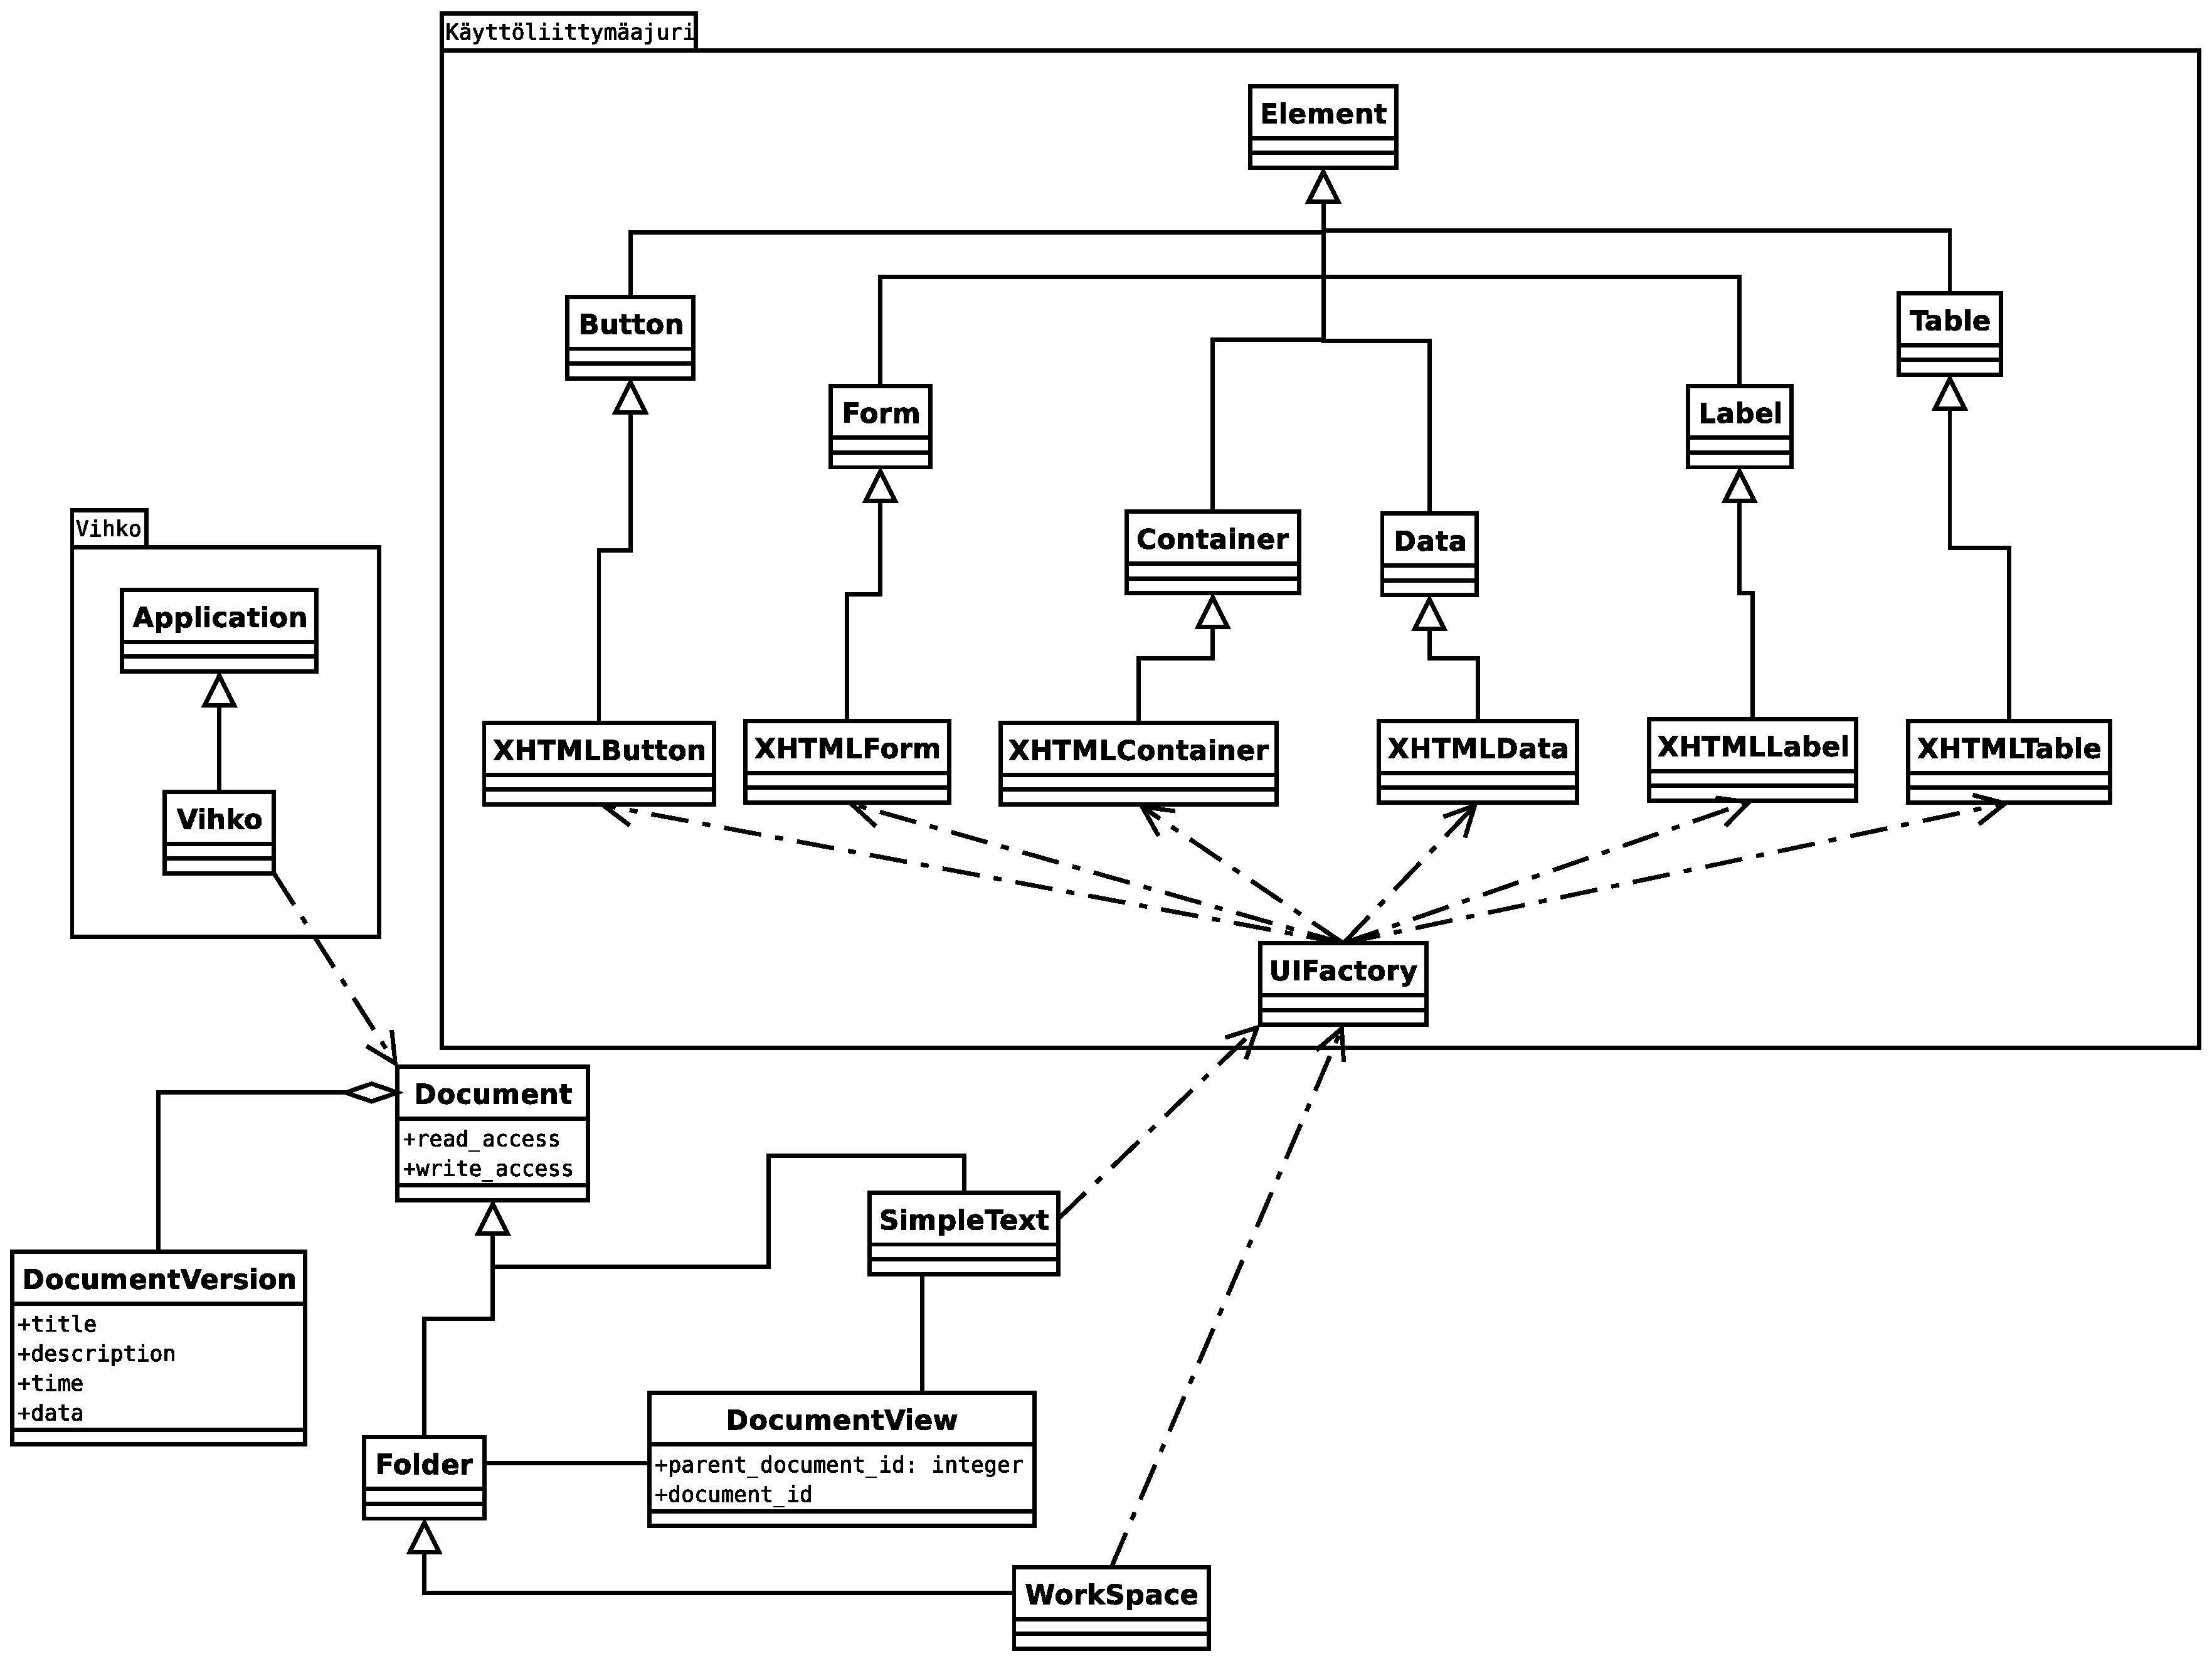
\includegraphics[width=\linewidth]{kuvat/vihko-schema-orig}
\caption{Alkuper�ist� suunnitelmaa Vihkon toteuttamiseksi}
\label{fig:vihko-schema-orig}
\end{kuva}

\begin{kuva}
\includegraphics[width=6.5cm]{kuvat/vihko-big-picture}
\caption{Osa toteutetusta Vihkon rakenteesta}
\label{fig:vihko-big-picture}
\end{kuva}

Noin kuukauden kehitysty�n j�lkeen k�vi kuitenkin selv�ksi, ett�
PHP-ymp�rist�n suorituskyky olioiden luomisessa ja tuhoamisessa oli
aika heikko ja lis�ksi k�ytetyst� arkkitehtuurista johtuen t�ydellisen
k�ytt�liittym�ajurin tekeminen alkoi varmistumaan liian ty�l��ksi siit�
saataviin etuihin verrattuna.

\section{Sovelluskehys avuksi}

Koska varsinaisen sovelluslogiikan ja k�ytt�j�n v�liss� on viel� useita
tasoja -- k�yh�n miehen k�ytt�liittym�ajuri, HTML ja CSS -- p��dyin
siihen johtop��t�kseen, ett� t�ydellist� k�ytt�liittym�ajuria ei
kannata tehd�. Lis�ksi, koska PHP rajaa ainakin toistaiseksi natiivin
k�ytt�liittym�n kehitt�misen mahdollisuuksia ei sen kehitt�misen
helpottamiseksi kannattanut t�ss� vaiheessa uhrata aikaa.

P��dyin loppujen lopuksi kuvassa \ref{fig:vihko-schema-current}
esitettyyn ratkaisuun. T�ss�kin luokkahierarkia on ensisilm�yksell�
v�hint��nkin outo, mutta ratkaisun taustalla kummittelee vaillinainen
oliotuki PHP-kieless�. T�t� kirjoittaessa PHP5 on jo ilmestynyt ja
siin� joitakin ongelmia onkin korjattu, mutta sen tuotantok�ytt��
kannattanee harkita aikaisintaan ensi vuonna.

\begin{kuva}
\includegraphics[width=\linewidth]{kuvat/vihko-schema-current}
\caption{Osa toteutetusta Vihkon rakenteesta}
\label{fig:vihko-schema-current}
\end{kuva}

Vihkon kehitt�misess� havaittujen ongelmien ratkaisemiseksi
sovelluskehyksen kehitt�minen vaikutti parhaalta ratkaisulta, koska
t�ll�in varsinaisen sovelluslogiikan koodi saadaan yksinkertaiseksi.
Sovelluslogiikkaan tuli mahdollisimman v�h�n sovelluksen toimintaan
liittym�t�nt� ohjelmakoodia joten uusien, samaa sovelluskehyst�
k�ytt�vien sovellusten teko nopeutuisi. My�s lokalisointiin tarvittava
logiikka on yhteinen eri sovellusten v�lill�. T�t� kirjoittaessa
vaikuttaa, ett� suurin osa tulevista sovelluksista voidaan kirjoittaa
Vihkon moduuleiksi.

Kaikki Vihkon moduulit perit��n luokasta \class{Document} (ks. kuva
\ref{fig:vihko-schema-current}) ja kaikki moduulit saavat oman
nimiavaruuden k�ytt�milleen parametreille. Esimerkiksi jos moduuli,
jonka id-numero on \code{251} asettaa sivulle parametrin, jonka nimi on
\code{foo}, k�ytet��n todellisena parametrin nimen� merkkijonoa
\code{p251xfoo}. Muunnos takaisinp�in tapahtuu automaattisesti
\class{Document}-luokan toimesta. Eri moduulien parametrit sijoitetaan
omiin nimiavaruuksiinsa sen vuoksi, ett� useita moduuleita olisi
mahdollista suorittaa rinnakkain samalla sivulla. Automaattinen
uudelleennime�minen mahdollistaa sen, ett� yksitt�ist� moduulia
ohjelmoitaessa ei tarvitse tarkistaa mit� nimi� muut moduulit
k�ytt�v�t. Lis�ksi \class{Document}-luokka yll�pit�� automaattisesti
istuntotietoa johon kuuluu globaali \code{session}-parametri, joka
sis�lt�� k�ytt�j�n ja tietokannan tunnistetiedot sek� varmenteen.
Lis�ksi kaikkiin toimintoihin lis�t��n t�ll� hetkell� k�yt�ss� olevan
moduulin tunniste ja edellisen k�yt�ss� olleen moduulin tunniste.
N�iden tietojen avulla moduulin kaikista toiminnoista palataan
oletuksena takaisin samaan moduuliin, mutta esimerkiksi
\emph{tallenna}-toiminnon j�lkeen voidaan palata edelliseen moduuliin
(joka usein on kansio).


\chapter{Peda.net"-hanke}

\begin{chapterquote}{Lainaus esiselvityksen johdannosta} Koulutus on
investointi tulevaisuuteen. T�m�n p�iv�n ratkaisut vaikuttavat
\mbox{10--20} vuoden aikaj�nteell� ty�el�m��n ja muuhun yhteiskuntaan viel�
\mbox{30--40} vuoden kuluttua. Toisaalta tulevaisuus, johon koulutuksen tulisi
lapsia ja nuoria valmentaa, on yh� nopeammin muuttuva ja vain lyhyell�
aikav�lill� ennakoitavissa. \end{chapterquote}

Peda.net\footnote{Peda.net on Jyv�skyl�n yliopiston rekister�ity
tavaramerkki.} sai alkunsa Jyv�skyl�n Yliopiston tekem�st�
telemaattisen opetusverkon hy�dynt�mismahdollisuuksien esiselvityksest�
vuonna 1996. Esiselvityksess� tutkittiin mahdollisuuksista luoda uusia
oppimisymp�rist�j� eri Keski"-Suomen kouluasteille. Esiselvitys
perusteli uusien ymp�rist�jen tarvetta seuraavasti:

\begin{quote} Oppiminen perustuu olemassa olevan tiet�myksen
jalostamiseen. Yksitt�isten tietojen ulkokohtainen muistaminen ei
edist� taitoa k�ytt�� tiet�myst��n itsen�isesti ja luovasti. Uusi
oppimisymp�rist� edellytt�� mahdollisuutta k�ytt�� monipuolisia
tietol�hteit� oma"-aloitteisesti. T�ss� tietoteknologia tarjoaa kaikille
kouluille ja jokaiselle oppilaalle aivan uudenlaisen mahdollisuuden
tiedon hankintaan ja kokemusten vaihtamiseen. \end{quote}

Esiselvityksen suosittelema PEDANET"-hanke k�ynnistyi vuonna 1997
Keski"-Suomen kuntien yhteisty�n�. Hankkeen ensimm�isen vaiheen
rahoitus jaettiin Keski"-Suomen liiton verkottumiseen varatuista
EU"-tuista. K�yt�nn�ss� hankkeen k�yt�nn�n toteutus oli hyvin kaukana
esiselvityksen sis�ll�st�, joka sis�lsi suunnitelman esimerkiksi
PEDANET"-hankkeen hallinnoimasta kouluverkosta. Eli hanke olisi
t�ll�isen tavoitteen mukaisesti vastannut koulujen internet"-yhteyksien
yll�pit�misest�. My�hemmin todettiin, ett� t�ll�inen teht�v� ei vastaa
yliopiston tavoitteita. \cite{pedanet:esiselvitys}

Hanke on toiminut alusta asti Jyv�skyl�n Yliopiston Koulutuksen
tutkimuslaitoksen (\alt{KTL}) alaisuudessa, jossa taustahenkil�n� on
ollut laitoksen nykyinen johtaja Jouni V�lij�rvi. Teknisen�
vastuuhenkil�n� toimi aluksi Jari Hautam�ki, joka oli ottanut teht�v��
varten virkavapaata normaalista ty�st��n Jyv�skyl�n teknillisen
oppilaitoksen opettajana. Hautam�ki otti ty�h�n avukseen silloisen
oppilaansa Juha Lahden, joka on jatkanut hankkeen ty�ntekij�n� t�h�n
p�iv��n asti.

\section{Pedanet vaihe I, 1997--1999}

Pedanet"-hanke k�ynnistyi Keski"-Suomen liiton, Jyv�skyl�n yliopiston,
Jyv�skyl�n ammattikorkeakoulun ja Telecom Finland Oy eli Telen v�lisen
aiesopimuksen allekirjoittamisella vuonna 1997. Aiesopimuksen mukaan
Pedanet tulisi muodostumaan kahdesta itsen�isest� osasta: oppilaitosten
v�lisest� verkosta sek� tietoverkkoon pohjautuvasta opetuksen
kehitt�misest�. \cite{pedanet:aiesopimus}.

Oppilaitosten v�lisen verkon yll�pito ja kehitt�minen j�i osin
toteutumatta ja Pedanet olikin mukana vain koordinoimassa Keski"-Suomen
koulujen verkottumista, mutta rahoituksen ja k�yt�nn�n j�rjestelyt
j�senkunnat hoitivat t�lt� osin itse. K�yt�nn�ss� Pedanetin ensimm�inen
vaihe muodostui kymmenest� pilottiprojektista
\cite{pedanet:julkaisematon-pilottisuunnitelma}. Maininnan arvoisesti
kaikki oppinaineiden sis�ll�ntuotantoon liittyneet projektit j�iv�t
pilottiprojektin tasolle. Vaikutti silt�, ett� opettajat eiv�t ehdi
varsinaisen kouluty�n sivussa tuottaa oppimateriaalia, mutta muiden
pilottien perusteella opettajat olivat kiinnostuneet olemassaolevan
materiaalin tarjolleasettamisesta verkkoon. Kymmenest� pilotista
pitk�aikaisemmiksi j�i vain nelj�:

\begin{description}

\item[Kyl�koulujen verkottuminen ja opetuksen monipuolistaminen,] jonka
tavoitteena oli edist�� haja"-asutusalueiden pienten ala"-asteen
koulujen edellytyksi� hy�dynt�� tietoverkkoja opetuksessa toimimalla
yhteisty�ss� kesken��n. T�ss� pilotissa olivat mukana muun muassa
Kekkil�n, Saarij�rven, Toivakan ja Joutsan koulut.

\item[Koulun Online "-ymp�rist�n luominen,] jonka tavoitteena oli luoda
uusi internetin v�lityksell� toimiva online"-palvelu, johon voidaaan
liitt�� koulun ja sen eri toiminnallisten ryhmien (luokat, opettajat,
henkil�kunta) tavoitteiden mukainen toiminta. T�ss� pilotissa olivat
mukana Vitikkalan ala"-aste ja J�ms�n koulu.

\item[Verkostokoulu valinnaisuuden monipuolistajana,] jonka tavoitteena
oli lis�t� valinnaisuutta pohjoisen Keski"-Suomen oppilaitokseissa
tarjoamalla niille opetusta ja sis�lt�j� yhteisen tietoverkon kautta.
T�ss� pilotissa olivat mukana kaikki pohjoisen Keski"-Suomen
oppilaitokset.

\item[Koulutustasojen yhteisty� -- p�iv�kodista kouluun,] jossa
tutkittiin p�iv�kodin ja peruskoulun v�lisen yhteisty�n
toteuttamistapoja. Tietoverkkoja pyrittiin k�ytt�m��n opettajien
ammmatillisen keskustelun ja asiantuntijuuden edist�miseksi, sek�
lasten kokemusten v�litt�misess� digitaalisia portfolioita hy�dynt�en.

\end{description}

Yhteisen� nimitt�j�n� n�ill� piloteilla oli ``Online''"-nimell�
kulkeneen verkkojulkaisuv�lineen k�ytt�. Juha Lahti r��t�l�i siit�
paremmin pienille lapsille soveltuvan version. Online
verkkojulkaisuv�lineen nimeksi tuli my�hemmin Verkkolehti, jonka uusin
versio on nykyisin Pedanetin toiseksi k�ytetyin ty�kalu.

Ty�kalujen merkitys johtuu todenn�k�isesti siit�, ett� koulujen
verkottuminen oli p��asiassa seurausta Opetushallituksen
Tietosuomi"-hankeen tavoitteista. Opetushallitus pyrki kannustamaan
opettajia hankkimaan tarvittavia taitoja tietoverkon k�ytt�miseen
opetuksessa. K�yt�nn�ss� tuohon aikaan tiedon julkaiseminen verkossa
vaati paljon teknist� ymm�rryst� ja Pedanetin helppok�ytt�iset ty�kalut
antoivat mahdollisuuden tuottaa sis�lt�� verkkoon ymm�rt�m�tt� teknisi�
yksityiskohtia. Paljon merkityst� on ollut ilmeisesti my�s sill�, ett�
Pedanetin ohjelmat ovat aina toimineet hankkeen palvelimilla, joten
koulujen ei ole tarvinnut asentaa niit� varten erillisi� sovelluksia. 
Varsinkin pienemmiss� kouluissa atk"-j�rjestelyist� vastaa usein
matematiikan tai fysiikan opettaja, joten aikaa suuriin
ohjelmistoasennuksiin ei yleens� ole.

Ensimm�isen vaiheen aikana projektissa ty�skenteliv�t p��asiassa Juha
Lahti tekniikasta vastaavana henkil�n�, joka my�s toteuttu
palvelinsovellusten ohjelmointia ja toimintaa koordinoi Pentti
Pirhonen, joka oli virkavapalla J�ms�n lukion rehtorin toimesta. Itse
toimin ensimm�isen vaiheen aikana hankkeessa p�tk�t�iss�
asevelvollisuuden suorittamisen j�lkeen vuonna 1998. Teht�viini kuului
www"-sivuston yll�pitoa ja palvelinohjelmistojen kehitt�mist�.
Pedanetin levitt�misest� vastasi t�h�n aikaa p��asiassa
T�ydennyskoulutuskeskus, joka koulutti Pedanet"-ty�v�lineiden k�ytt��.

Samoin ensimm�isen vaiheen aikana nimi Pedanet muuttui jo
ep�virallisesti Peda.netiksi ja internet"-osoite muuttui sijainnista
\url{http://pedanet.jyu.fi/} uuteen osoitteeseen
\url{http://peda.net/}, jossa se nykyisinkin toimii.

\subsection{Hankkeen ensimm�isen vaiheen sovellustuotantoa}

Kuten yll� mainitsin, Juha Lahden Online"-ymp�rist� oli merkitt�v�ss�
roolissa onnistuneissa pilottiprojekteissa. T�m� Online"-nimell�
kulkenut ymp�rist� nimettiin my�hemmin Verkkolehdeksi ja se kehittyi
ensimm�isen vaiheen aikana seuraavasti:

\begin{ol}

\item Vitikkalan ala-asteella oli kehitetty ja kokeiltu erilaisia
pieni� ohjelmia opetusty�n tueksi. N�iden perusteella oli tehty
yksinkertainen www"-sivujen tuottamisymp�rist�, johon lis�si siihen
tiedostojen l�hett�mistoiminnon (\alt{file upload}). Tiedostojen
l�hett�minen oli tuolloin ilmestyneiden www"-selainten uusi ominaisuus.
Aikaisemmin koulun www"-sivujen yll�pidossa piti kirjoittaa
HTML"-kielinen sivun kuvaus k�sin ja p�ivitt�� sivut
FTP"-tiedonsiirtosovelluksella. T�m� oli ensimm�inen Peda.netin
tarjoama ty�v�line, jota muutama koulu k�ytti. Teknisesti ty�kalu oli
toteutettu Perl"-ohjelmointikielell� ja muutokset tehtiin suoraan
tiedostoj�rjestelm��n.

\item My�hemmin samana vuonna Juha uudelleenkirjoitti verkkolehden
ohjelmakoodin helpommin yll�pidett�v��n muotoon. Toiminnallisia
ongelmia korjattiin.

\item Verkkolehdest� tehtiin kolmas versio vuonna 1999, jossa tiedot
tallennettiin SQL"-tietokantaan. J�rjestelm� toimi
Perl"-ohjelmointikielell� ja tietokannan teht�v�� hoiti miniSQL. T�m�n viel� ``Online''"-nimell� julkaistun version pilotointi ja esittely tapahtui toukokuussa 1999.
\end{ol}

Verkkolehden lis�ksi oli k�yt�ss� Jyv�skyl�n yliopistolla Cum Laude
"-ty�projektina syksyll� 1999 valmistunut OPSpro"-sovellus. Osa
Keski"-Suomen koulusta k�ytti my�s 1999 kirjoittamaani
Kurssitarjotin"-sovellusta. Peda.netin toiminnassa oli jo tuolloin
havaittavissa nopea ohjelmistonkehityksen tahti; olennaista oli saada
jotakin valmiiksi ja palautetta k�ytt�jilt� -- t�ss� tapauksessa
p��asiassa pilottiprojekteihin osallistuneilta opettajilta. N�iden
lis�ksi Pedanet tarjosi muun muassa verkkoilmoitustaulun ja
keskustelufoorumin opettajien k�ytt��n. Hankkeen tuottamat sovellukset
tarjottiin Keski"-Suomen koulujen k�ytt��n ensimm�isen vaiheen aikana
ilmaiseksi.



\section{Peda.net vaihe II, 2000--2001}

Pedanet"-hankkeen ensimm�isen vaiheen rahoitus kesti vuoden 1999
loppuun asti. KTL haki vuonna 1999 rahoitusta Pedanet"-hankkeen toista
vaihetta varten. Hankesuunnitelman perusteluissa luki muun muassa:

\begin{quote} Syntyneiden palveluiden laajamittainen k�ytt��notto ja
edelleen kehitt�minen voidaan parhaiten turvata vuosille 2000--2001
ajoittuvalla uudella hankkeella, joka uuden valtakunnallisen
tietoyhteiskuntastrategian mukaisesti profioidaan selv�sti verkon
sis�lt�jen ja palvelujen kehitt�mishankkeeksi. \end{quote}

Hankesuunnitelman 12 osaprojektista vain muutama jatkoi toisen vaiheen
rahoituksen loppumisen j�lkeen:

\begin{description}

\item[Liikennekasvatuksen verkkopalvelu,] jonka tavoitteena oli luoda
yhteisty�ss� Liikenneturvan kanssa koulujen liikenneasvatusta tukeva
verkkopalvelu. Palvelu toimii osoitteessa
\url{http://liikenne.peda.net/} ja sivuston yll�pito on jatkunut t�h�n
p�iv��n saakka.

\item[Oppiaineiden verkkoymp�rist�t,] jonka tavoitteena oli kehitt��
opettajien tarpeisiin oppiainekohtaisia ty�kaluja syyskuussa 1999
l�hetetyn kyselyn perusteella. K�yt�nn�ss� palautteen perusteella
kehitettiin Verkkover�j�n olemassaolevia moduuleita tai luotiin uusia, paremmin tarpeeseen sopivia.

\item[Verkkotiedottamisj�rjestelmien kehitt�minen,] jonka tavoitteena
oli kartoittaa koulutoimen tiedottamistarpeet ja tarjota
verkkotiedottamisymp�rist�j�. K�yt�nn�ss� tiedotus hoidettiin
Verkkover�j�n moduulien avulla. My�s Verkkolehte� k�ytettiin joissakin
kouluissa.

\item[EU"-koulutusohjelmien verkkopalveluiden kehitt�minen,] jonka
keskeisen� osana oli tukea Sokrates"-koulutusohjelman eri osioissa
mukana olevia kouluja. Koska koulut sijaitsivat maantieteellisesti
kaukana toisistaan eiv�t oppilaat voineet n�hd� toisiaan kasvotusten
vaan kommunikointi tapahtui oppimisymp�rist�jen kautta. K�yt�nn�ss�
verkkolehdest� tehtiin t�m�n projektin puitteissa englanninkielinen
versio projektin tarpeisiin.


\item[Keski"-Suomen kouluverkon laajakaistainfrastruktuurin kehitys,]
joka k�yt�nn�ss� koordinoi kuntien verkottumishankkeita. Peda.net auttoi
muun muassa rahoituksen hakemisessa Opetushallitukselta ja tiedotti eri
rahoitusvaihtoehdoista. Peda.net ei sin�ns� toteuttanut yhteyksien
rakentamista.

\end{description}

\subsection{Hankkeen toisen vaiheen sovellustuotantoa}

Hankkeen toisen vaiheen aikana kehitettiin kouluille useita uusia
sovelluksia. My�s aikaisemmin k�yt�ss� olleita ty�kaluja, Verkkolehte�
ja OPSpro"-sovellusta p�ivitettiin. Verkkolehden vuoden 2000 lopussa
valmistunut nelj�s versio, josta k�ytt�j�t k�yttiv�t vain nimityst�
\emph{Verkkolehti}, oli itse asiassa Juha Lahden opinn�ytety�. T�m�
verkkolehden versio pysyikin k�yt�ss� Verkkolehden viidenteen, vuonna
2004 julkaistuun versioon -- t�ll� kertaa virallisesti
\emph{Verkkolehti 2} -- saakka.

Toisen vaiheen aikana suunnittelin ja toteutin OPSpro"-sovelluksen
toisen version, joka sai nimekseen OPSpro2. My�hemmin, vuonna 2001,
tein ensimm�isen version Verkkover�j�st�, joka pysyikin k�yt�ss� sen PHP"-ohjelmointikielell� uudelleekirjoittamiseen saakka vuonna 2004.

Juha teki viel� OSPpro"-sovelluksesta syksyll� 2001 Verkkolehden
ohjelmakoodin pohjalta yksinkertaisemman version. T�m� OPSpro"-versio
on viel� nykyisinkin k�yt�ss�.

%ver�j�n v3 (virallisesti "2") kes�-joulu 2003 (php, mysql)

%verkkolehti 5 (virallisesti "2"), 2004

%sosiaalinen innovaatio

% Omat softat:
% Toisen asteen kurssitarjotin (1999)
% OPSpro2 (2000)
% Verkkover�j� (ty�nimi: Portaali, 2001)
% Verkkover�j� 2 (ty�nimi: Portal2, 2002)
% YALE2 eli \alt{Yet Another Learning Environment 2} (2003)
% Oppimappi (ty�nimi: Vihko, 2003--2004)

\section{Hankkeen rahoitus loppui, uusi toimintamalli edess�}

Pedanet"-hankkeen toinen vaihe p��ttyi vuoden 2001 lopussa ja vakiintui
silloin Jyv�skyl�n yliopiston Koulutuksen tutkimuslaitoksen
koordinoimaksi tutkimus- ja kehitt�mishankkeeksi -- nyt hankkeen nimen
kirjoitusasuksi vakioitiin virallisestikin Peda.net. T�st� eteenp�in
Peda.net pyrki toimimaan omarahoitteisena ja onkin nykyisin siihen
tavoitteeseen p��ssyt kouluverkon j�senilt� ker�ttyjen vuosimaksujen
turvin. Siirtym�vaiheessa omarahoitteiseksi Koulutuksen
tutkimuslaitoksen rooli hankkeessa oli merkitt�v�.

Peda.net"-kouluverkon j�senet saavat vuosittaisen j�senmaksun
vastineena vapaan k�ytt�oikeuden opetusty�ss� kaikkiin Peda.netin
kehitt�miin ja yll�pit�miin sovelluksiin ja p��sev�t halutessaan
osallistumaan uusien sovellusten kehitt�miseen. Peda.netill� oli vuoden
2004 tammikuussa j�senin� 70 kuntaa (j�senkunnan kaikilla kouluilla on
vapaa k�ytt�oikeus kaikkiin Peda.net"-verkkoty�v�lineisiin) ja sen
lis�ksi yksitt�isi� kouluja tai oppilaitoksia oli yli 50 kunnassa.
J�senen� on my�s erilaisia hankkeita ja projekteja. Toiminta on voittoa
tavoittelematonta.

\section{Tutkimusty�}

Peda.net"-kouluverkko toimii Koulutuksen tutkimuslaitoksessa Tietoverkot
oppimis- ja ty�ymp�rist�iss� "=tutkimusryhm�n yhteydess�. Tutkimusryhm�n
tavoitteena on tarkastella teknologian ja virtuaalisten
oppimisymp�rist�jen mahdollisuuksia oppimisen ja opetuksen tukena.
Tutkimusryhm�n tekem� tutkimus on yht��lt� monitieteist�,
teoreettisesti painottunutta perustutkimusta sek� toisaalta
k�yt�nn�llist� l�ht�kohdista nousevaa kehitt�mistutkimusta.

Peda.net kouluverkkoon liittyv� tutkimus on kehitt�mistutkimusta, joka
tapahtuu l�heisess� yhteisty�ss� koulujen ja opettajien kanssa. Eri
oppilaitosten ja organisaatioiden henkil�st�n lis�ksi
tutkimusyhteisty�ss� on mukana my�s muita alan kansallisia ja
kansainv�lisi� asiantutkijoita.

\section{Kokonaiskuva nykytilanteesta}

Hankkeessa ty�skentelee nykyisin kolme t�ysip�iv�ist� ty�ntekij��:
Jaana Kettunen, Juha Lahti ja Jarkko Lampinen. Toimin itse nelj�nten�
ty�ntekij�n�, toistaiseksi puolip�iv�isen�. Hankkeen Linux"-palvelimien
yll�pidosta vastaavat Juha Lahti ja Mikko Rantalainen.

[*** Liitteiss� X ja Y on esitetty Peda.net"-hankkeen tilastotietoja sek� toimintasuunnitelmaa. ***]

%\newpage{} % HACK!

\section{Hankkessa kehitt�mi�ni sovelluksia ja prototyyppej�}

Kuten aikaisemmin mainitsin, olen ty�skennellyt Peda.netiss� syksyst�
1998 alkaen, joten kokemusta erilaisista selaink�ytt�isist�
sovelluksista on kertynyt jo useammalta vuodelta. K�sittelen
seuraavassa kehitt�m�ni sovellukset aikaj�rjestyksess�.

\subsection{Toisen asteen kurssitarjotin}

Toisen asteen kurssitarjotin kehitettiin Peda.netin toimesta kes�ll�
1999, Jyv�skyl�n Ammattioppilaitoksen (nykyinen \alt{Jyv�skyl�n
ammattikorkeakoulu}) ja sen kanssa yhteisty�ss� toimivien koulujen
k�ytt��n. Sovelluksen kehitt�mist� koordinoi Peda.netin puolesta Pentti
Pirhonen ja kurssitarjottimen k�ytt�ji� edusti Vuokko Pennanen.

Sovelluksen taustalla oli samalla nimell� tuotettu paperiversio eri
oppilaitosten j�rjest�mist� kursseista. Eri oppilaitoksissa,
k�yt�nn�ss� ammattikouluissa ja lukioissa, j�rjestettiin kursseja,
joille muiden oppilaitosten oppilaat saattoivat osallistua. Tavoitteena
oli tehostaa toiminnan tiedottamista ja organisoida kursseille
ilmoittautumista s�hk�isell� ty�kalulla. Toisen asteen kurssitarjotin
sis�lsi samat tiedot kuin paperiopaskin. Lis�ksi siin� oli
yll�pitok�ytt�liittym� uusien kurssien, koulujen ja opettajien
sy�tt�miseen, muokkaamiseen ja poistamiseen, sek�
ilmoittautumisj�rjestelm� eri kursseille hakemiseksi.

Teknisesti Toisen asteen kurssitarjotin py�ri Linux"-palvelimella
Perl"-ohjelmointikielell� toteutettuna. Tietokannan teht�v�� hoiti
miniSQL"-ohjelmisto samalla koneella. Kun ottaa huomioon, etten ollut
t�t� sovellusta ennen tehnyt edes yksinkertaista CGI"-sovellusta,
t�ytyy olla tyytyv�inen lopputulokseen. Ohjelman perusrakenne perustui
osin Verkkolehden vuonna 1999 tehtyyn versioon.

Kurssitarjotin kehitettiin siihen aikaa yleiseen (selaink�ytt�isten
sovellusten) tyyliin, jossa ohjelman toiminta ja k�ytt�liittym�n
toimintaan liittyv� koodi oli sidottu melko tiukasti toisiinsa. Lis�ksi
normaali tietojen selailu "=k�ytt�liittym� ja yll�pitok�ytt�liittym�
toimivat omina sovelluksinaan k�ytt�en yhteist� tietokantaa. Ohjelman
yll�pito todettiin hankalaksi ohjelman heikon rakenteen,
miniSQL"-tietokannan rajoittuneisuuden ja kokonaisuuden sirpaleisuuden
vuoksi (selailu ja yll�pito k�yttiv�t osittain poikkeavia
k�ytt�liittymi�, mik� puolestaan koettiin huonona k�ytett�vyyten� --
t�m�n korjaaminen taas oli ty�l�st� ohjelman huonohkon teknisen
rakenteen seurauksena). Sovellukseen tehtiin pieni� korjauksia syksyll�
2000, ja silloin virallinen nimi oli ``Toisen asteen yhteys'' ja
yhteyshenkil�ksi oli vaihtunut Taina Roivainen. Uutta, t�ysin korjattua
versiota ei alettu koskaan tekem��n, vaan seuraavana projektina
siirryin kehitt�m��n OPSpron uutta versiota. Peda.netin kehitt�m�n
kurssitarjottimen k�ytt� loppui kes�ll� 2001.

\subsection{OPSpro2"-prototyyppi}

\begin{quote} Opetussuunnitelman kehitt�misen eli OPS"-ty�n tulisi olla
koulussa jatkuva, p�ivittyv� prosessi. OPSpro on helppok�ytt�inen
ty�v�line opetussuunnitelman tekemiseen, yll�pit�miseen ja
julkaisemiseen. Ty�v�line mahdollistaa mm. asiantuntijoiden ja
vanhempien osallistumisen sek� hallinnon lomakkeiden ja asiakirjojen
jakamisen. OPSprossa voit helposti monipuolistaa ulkoasua ja sis�lt��
kuvilla sek� ��ni- ja videoleikkeill�. \\
\mbox{}\hfill\mbox{---~\emph{OPSpro"-esittely}} \end{quote}

\begin{kuva}
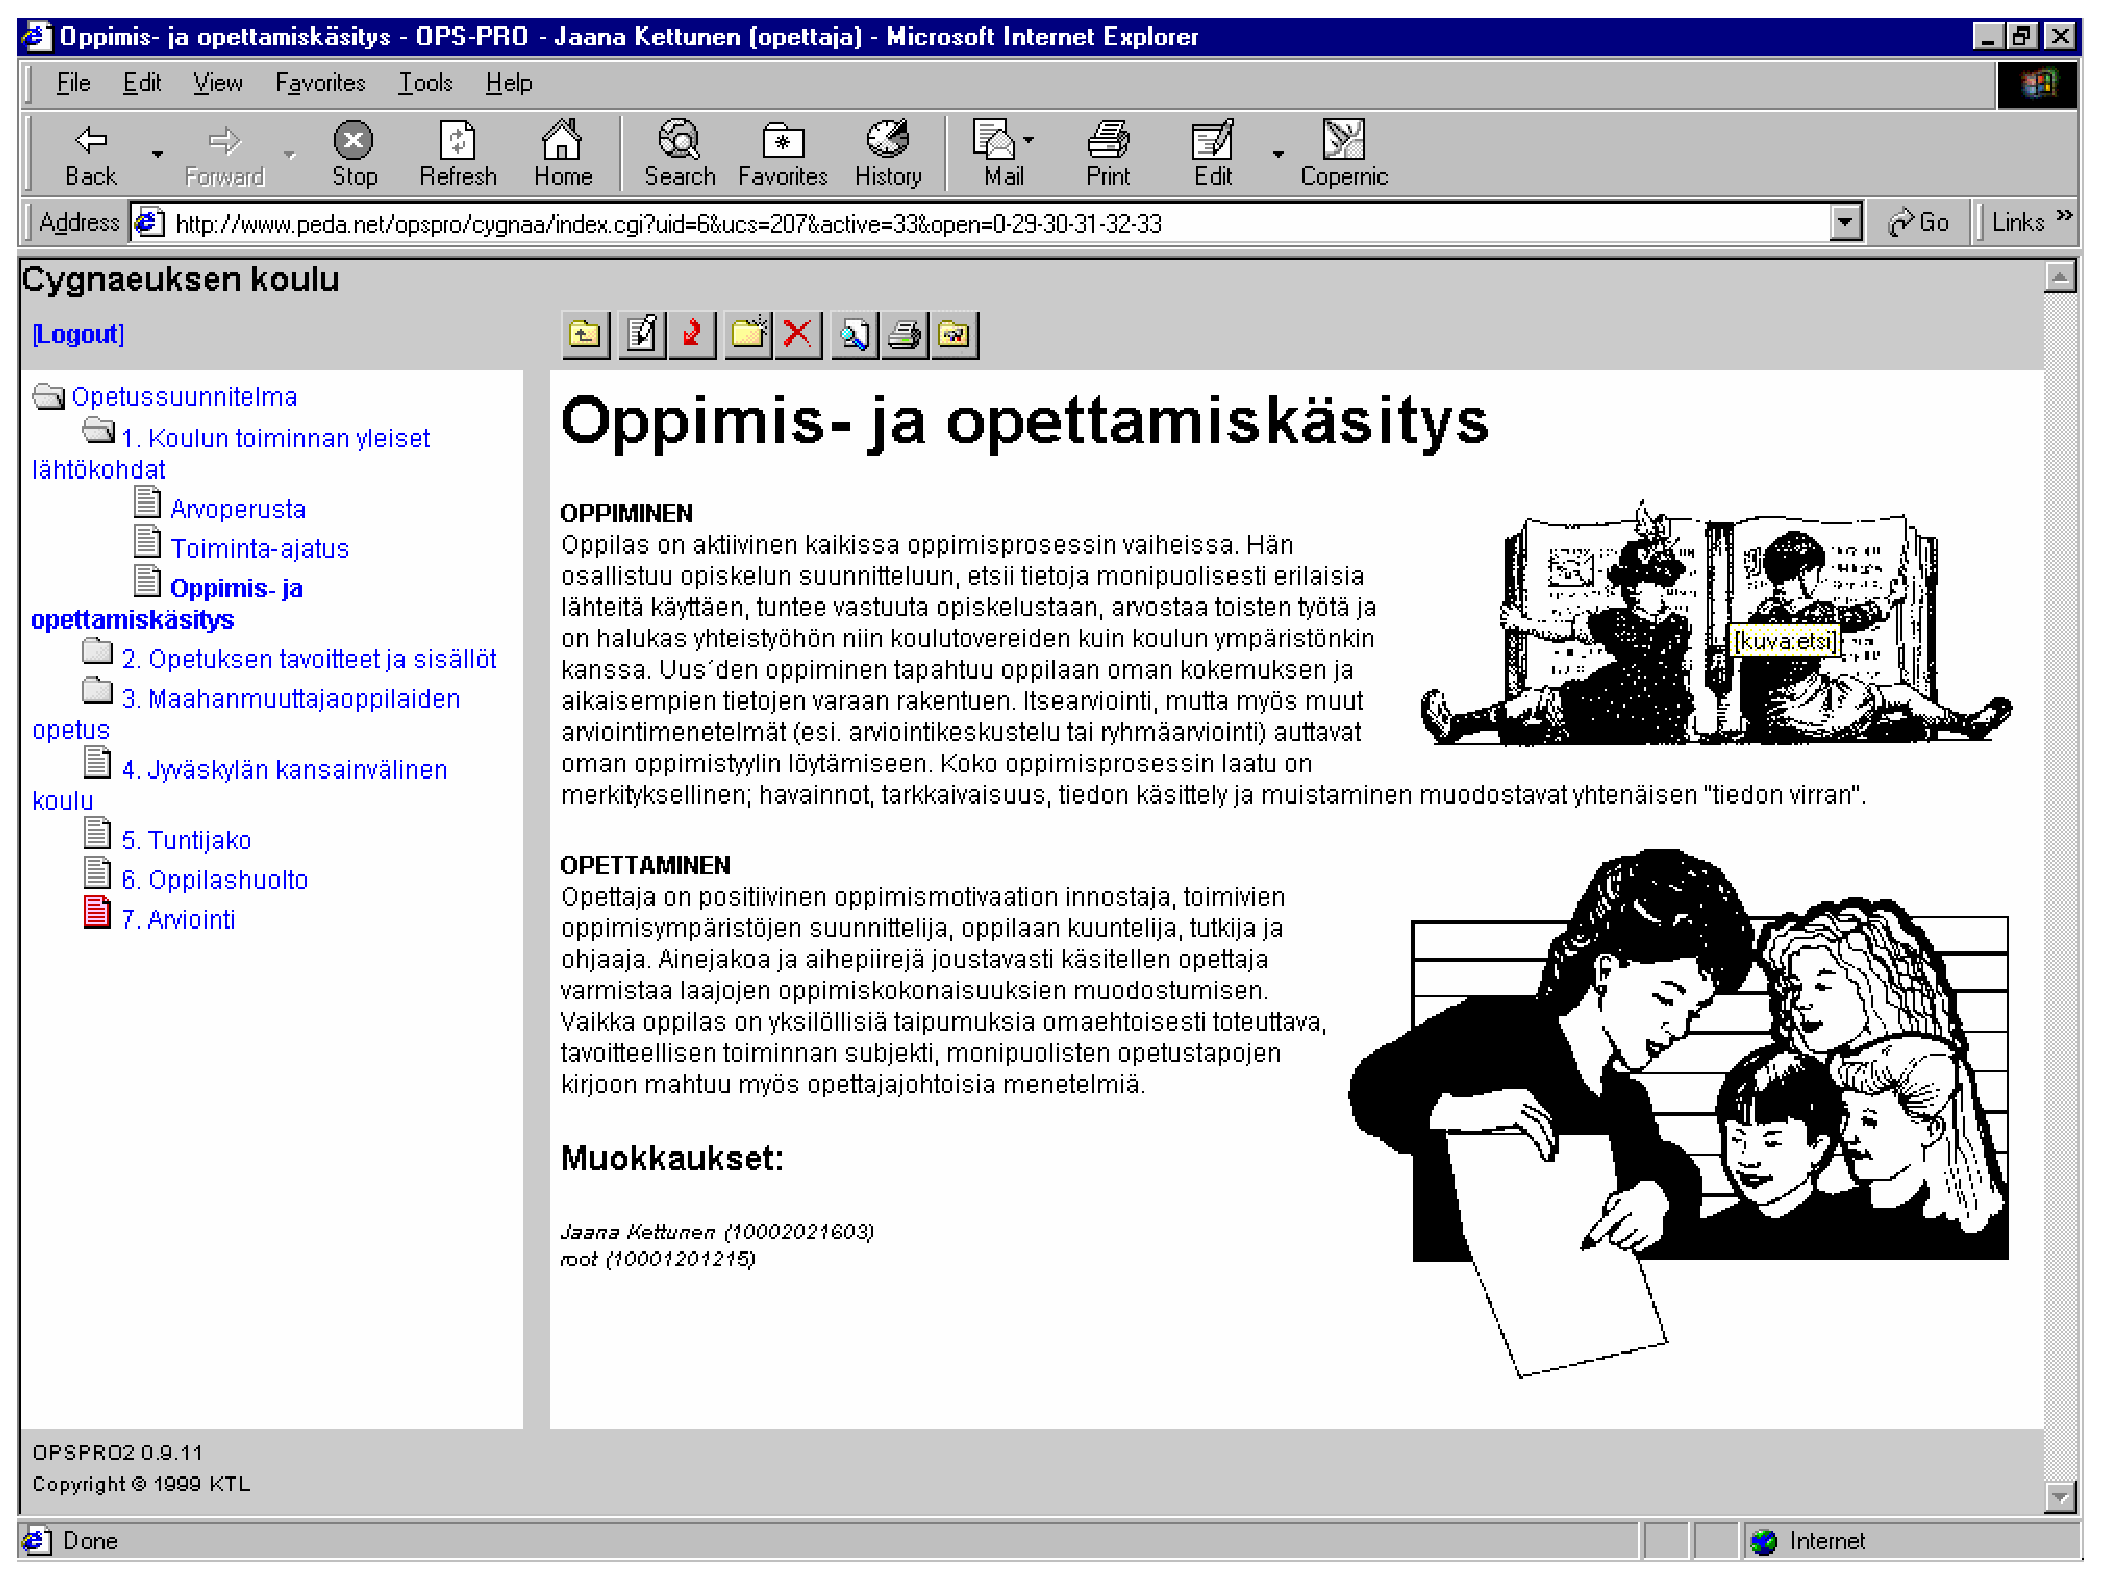
\includegraphics[width=11.5cm]{kuvat/opspro21}
\caption{Kuva OPSpro2"-prototyypin k�ytt�liittym�st�}
\end{kuva}

OPSpro eli opetussuunnitelmaprosessori, on hajautettu, rakenteisen
dokumentin tuottamissovellus. Koska jokaisella koululla tulee olla oma,
yksil�llinen opetussuunnitelma, ja toisaalta opetussuunnitelman
jokainen osa on parhaimmillaan t�ysin erillinen osuus (esimerkiksi
kuvaus englanninkielen opetuksesta yl�asteella) voi dokumentin eri
osia kirjoittaa samanaikaisesti useat eri henkil�t. OPSpron avulla
esimerkiksi �idinkielen opettaja voi kirjoittaa ja yll�pit��
opetussuunnitelman �idinkielen osuutta samaan aikaan, kun matematiikan
opettaja vastaavasti yll�pit�� omaa osuuttaan. OPSpro huolehtii
automaattisesti rakenteen yll�pit�misest� (eli �idinkieli ja englanti
ovat koko opintosuunnitelman alilukuja) ja koko dokumentin
kokoamisesta. T�ll�in dokumentin eri osia ei tarvitse l�hett��
esimerkiksi s�hk�postilla koko dokumentin kokoamisesta vastaavalle
henkil�lle, joka koostaisi koko dokumentin esimerkiksi MS Word
"=tekstink�sittelyohjelmalla. Ohjelman nykyisin k�yt�ss� olevalla
versiolla on kirjoitettu ongelmitta yli 500 sivun dokumentteja.

OPSpro ei sin�ns� pakota juuri opetussuunnitelman tekemiseen, vaikka
osa k�ytt�liittym�ss� k�ytetyist� termeist� siihen suuntaan viittaakin.
Kyseess� on pikemminkin yhteisty�ss� tuotettavien rakenteisten
dokumenttien kirjoittamiseen suunniteltu ty�kalu.

Ensimm�inen OPSpro oli kehitetty vuonna 1999 Jyv�skyl�n yliopiston
tietotekniikan laitoksen Cum Laude "=ty�projektina. T�m�n sovelluksen
tekninen toteutus todettiin kuitenkin my�hemmin selv�sti
riitt�m�tt�m�ksi. Teht�v�kseni j�i kehitt�� samaan ideaan perustuen
parempi versio kes�ll� 2000. T�m� versio j�i loppujen lopuksi
prototyypiksi, jolla tehtiin joitakin opetussuunnitelmia
pilottiprojekteina. Koulut eiv�t olleet viel� t�ss� vaiheessa valmiita
er�isiin OPSpro2:n ominaisuuksiin: erityisesti k�ytt�jien hallinta
tuotti ongelmia. Muissa ty�kaluissa oli tuohon aikaan yll�pitoon vain
yksi salasana koko koulua kohden ja t�h�n verrattuna usean
k�ytt�j�tunnuksen yll�pito oli liian vaativaa. Samoin rakenteisen
dokumentin kappaleiden oikeuksien hallinta osoittautui liian vaikeaksi
(ks. esim. kuva \ref{fig:opspro2-yllapito}).

\begin{kuva}
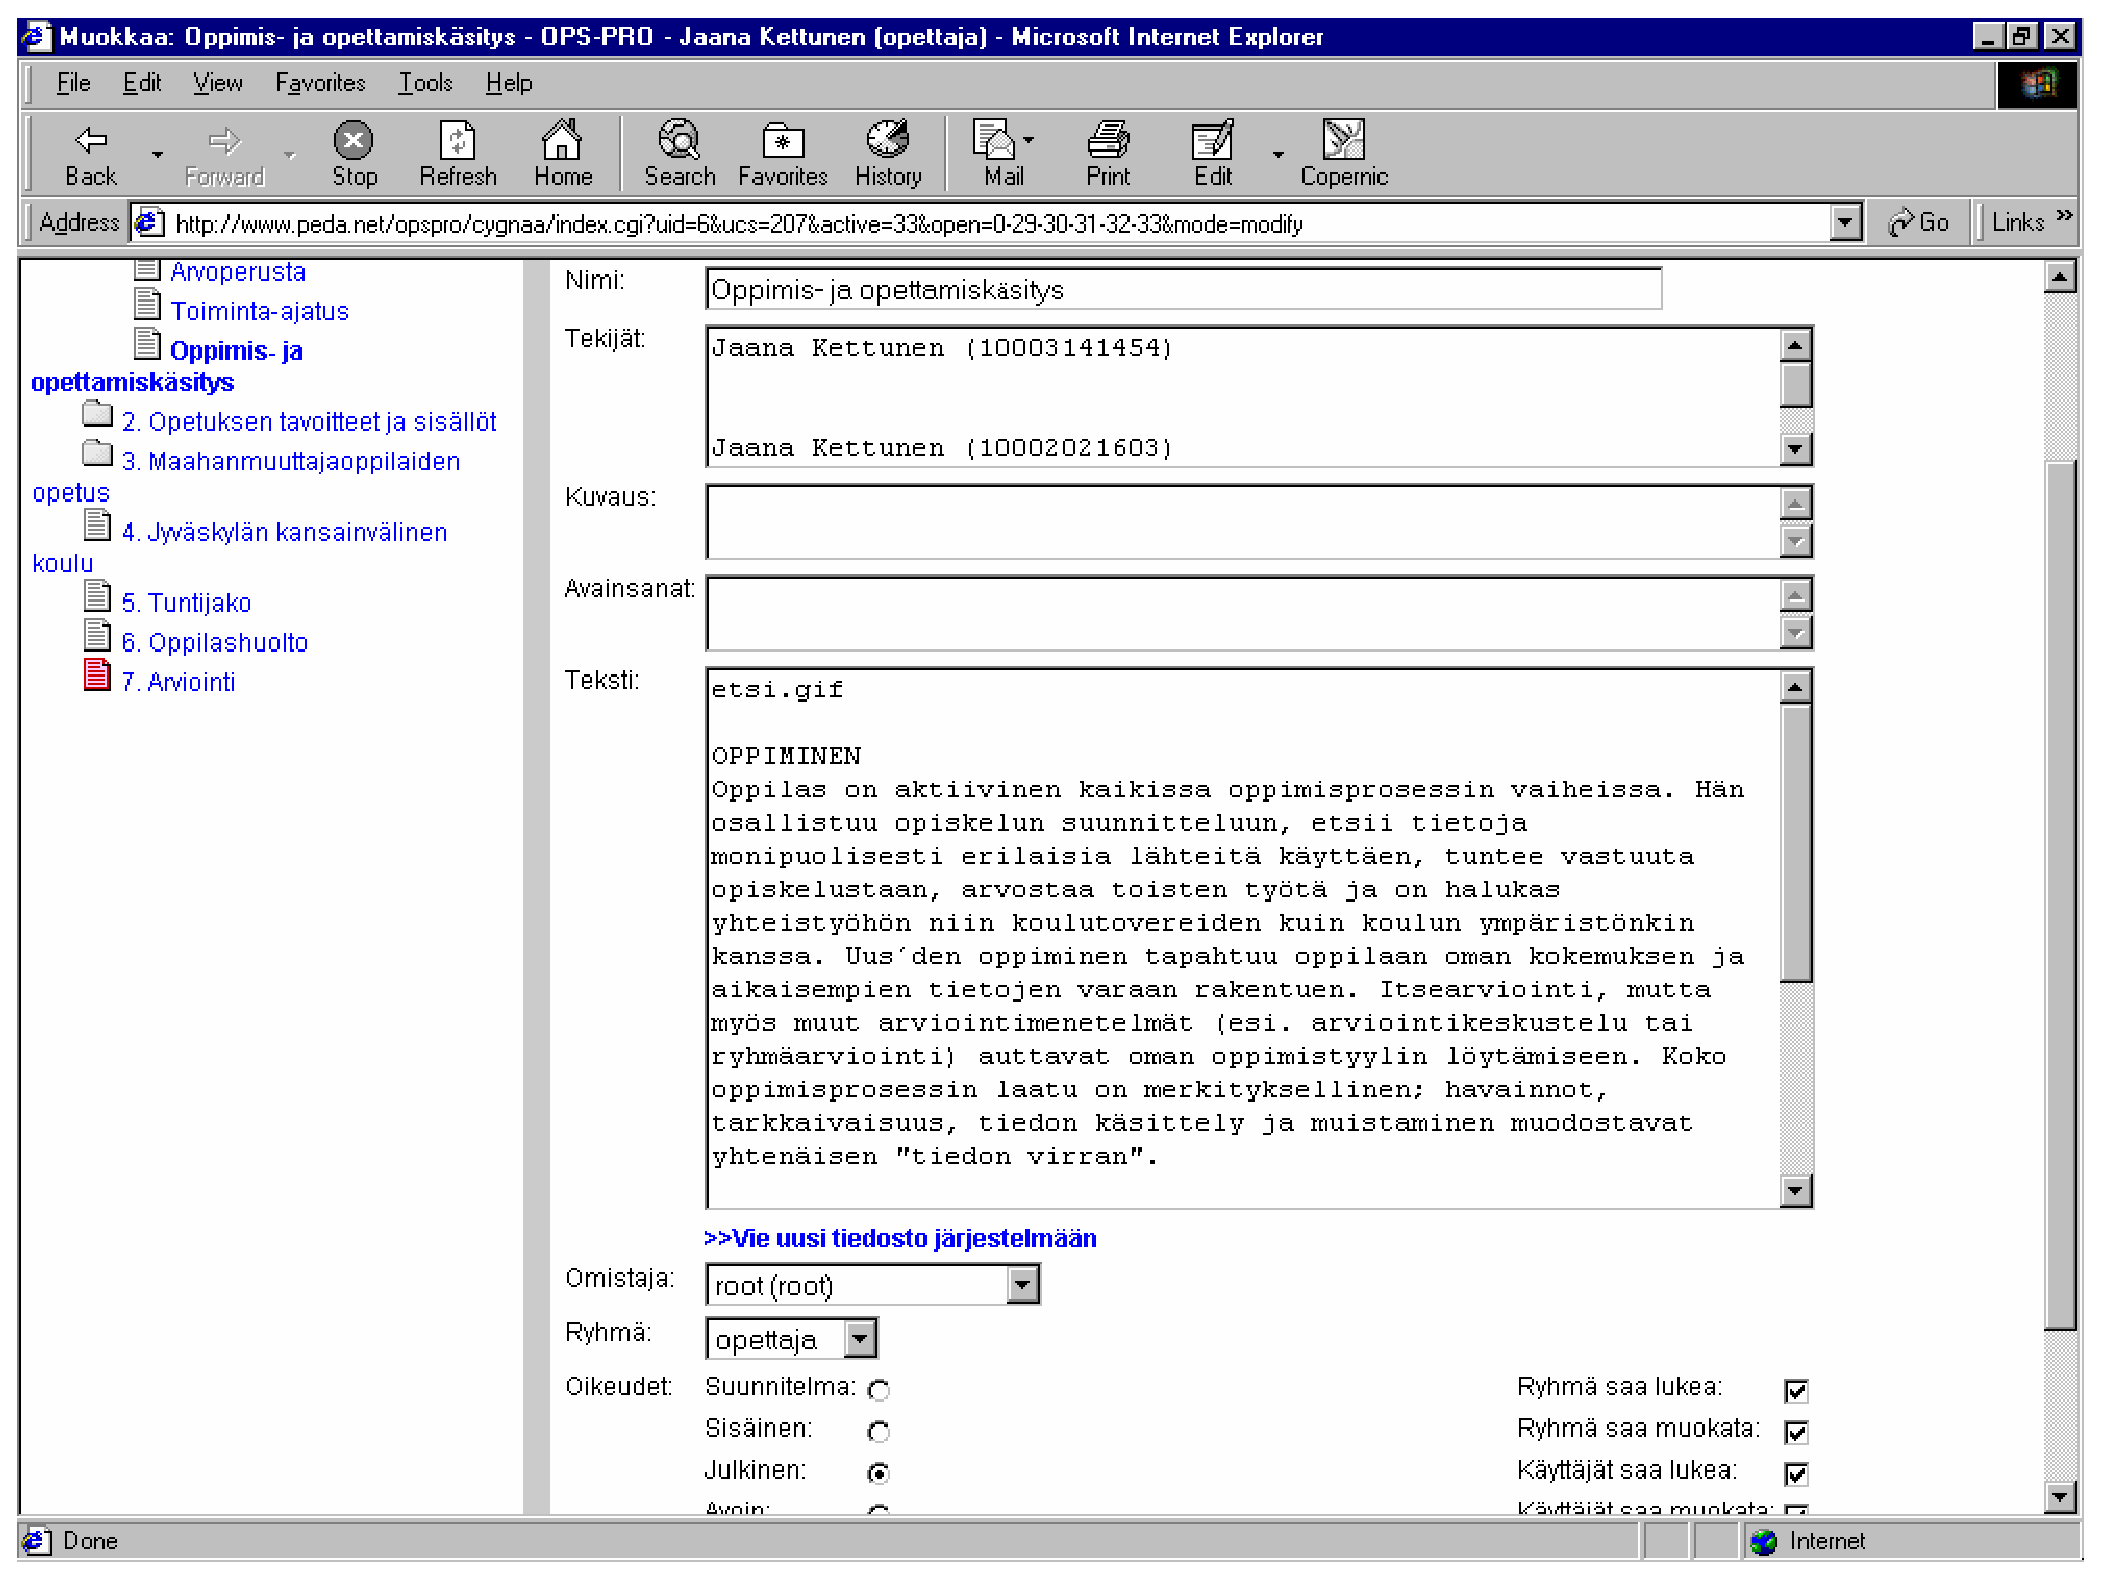
\includegraphics[width=11.5cm]{kuvat/opspro22}
\caption{Kuva OPSpro2"-prototyypin yll�pidon k�ytt�liittym�st�}
\label{fig:opspro2-yllapito}
\end{kuva}

Lis�ksi ohjelma toteutettiin Perl"-ohjelmointikielell�
miniSQL"-tietokannan p��lle. MiniSQL"-tietokannan nopeus ja vakaus
tekiv�t siit� teknisesti huonon alustan. Peda.netin kaikki ty�kalut on
sittemmin p��tetty toteuttaa PHP"-ohjelmointikielell� yll�pidon ja
sovellusten my�hemm�n integroinnin helpottamiseksi.

Toiminnallisesti sovellus pystyi tekem��n suurimman osan siit�, mit�
nykyisinkin k�yt�ss� oleva versio. Se tarjosi jopa enemm�n
mahdollisuuksia k�ytt�j�n suorittamaan r��t�l�intiin koulukohtaisesti,
erityisesti k�ytt�liittym�n osalta. K�yt�nn�ss� k�ytt�liittym�n
r��t�l�inti osoittautui kuitenkin liian vaikeaksi tavalliselle
opettajalle tai koulun atk"-yll�pit�j�lle (joka yleens� on
todellisuudessa matematiikan tai tietotekniikan opettaja). Lis�ksi
havaittiin, ett� Peda.netin k�ytt�jille sovelluksen ulkon�k� ei ollut
merkitt�v� tekij� -- kaikki k�ytt�j�t tyytyiv�t poikkeuksetta
oletusulkon�k��n. OSPpro2 matki my�s k�ytt�liittym�n ulkoasun puolesta
Microsoft Windows "=k�ytt�j�rjestelm��, mink� seurauksena sovelluksen
k�ytt�liittym� poikkesi voimakkaasti totutusta esimerkiksi Apple MacOS
"- k�ytt�j�rjestelm�n k�ytt�jille. Havaittiin my�s, ett�
k�ytt�liittym�n toimintavaihtoehtojen esitt�minen pelk�st��n ikonien
avulla ei ollut riitt�v�n selke��.

Nykyisin k�yt�ss� oleva OPSpron versio on Juha Lahden
PHP"-ohjelmointikielell� ohjelmoima ja se toimii
MySQL"-tietokantaohjelmistolla. Sovelluksen ohjelmakoodi on osin sama
Verkkolehden aikaisemman version kanssa. Tammikuussa 2004 sovelluksella
toimitettuja opetussuunnitelmia oli noin 600.

\subsection{Verkkover�j�}

\begin{kuva}
%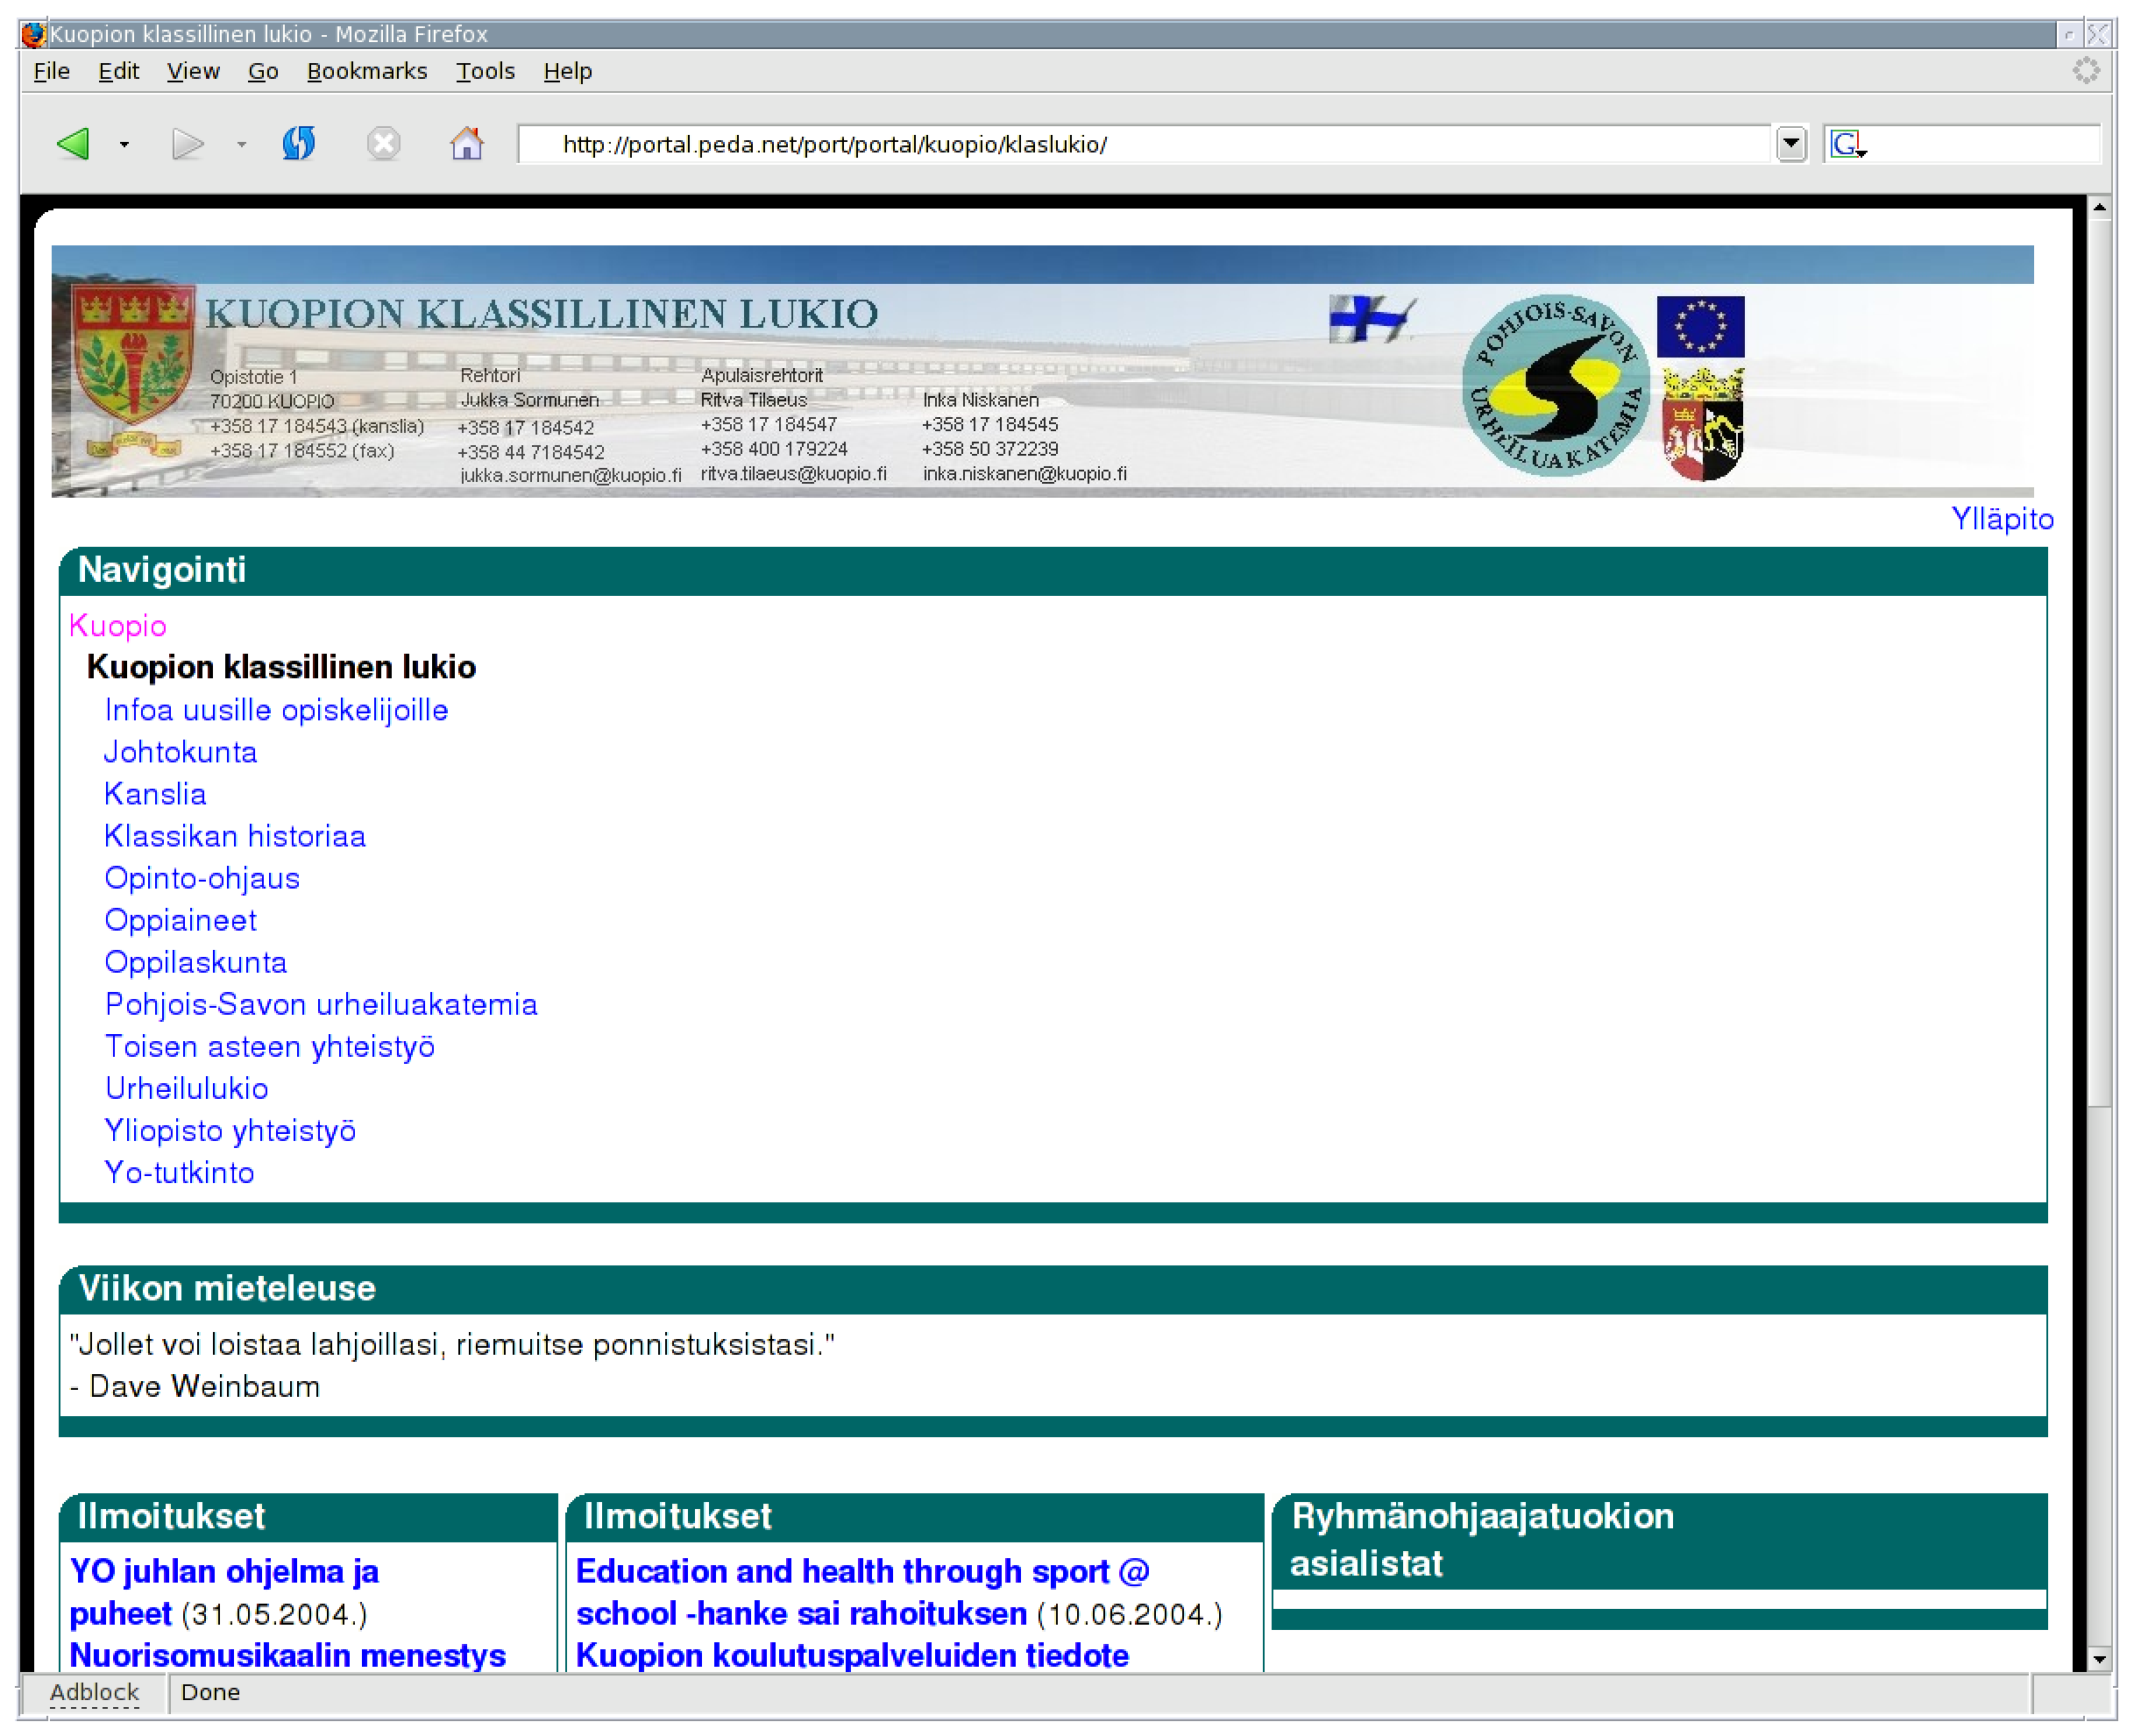
\includegraphics[width=\linewidth]{kuvat/lukio1}
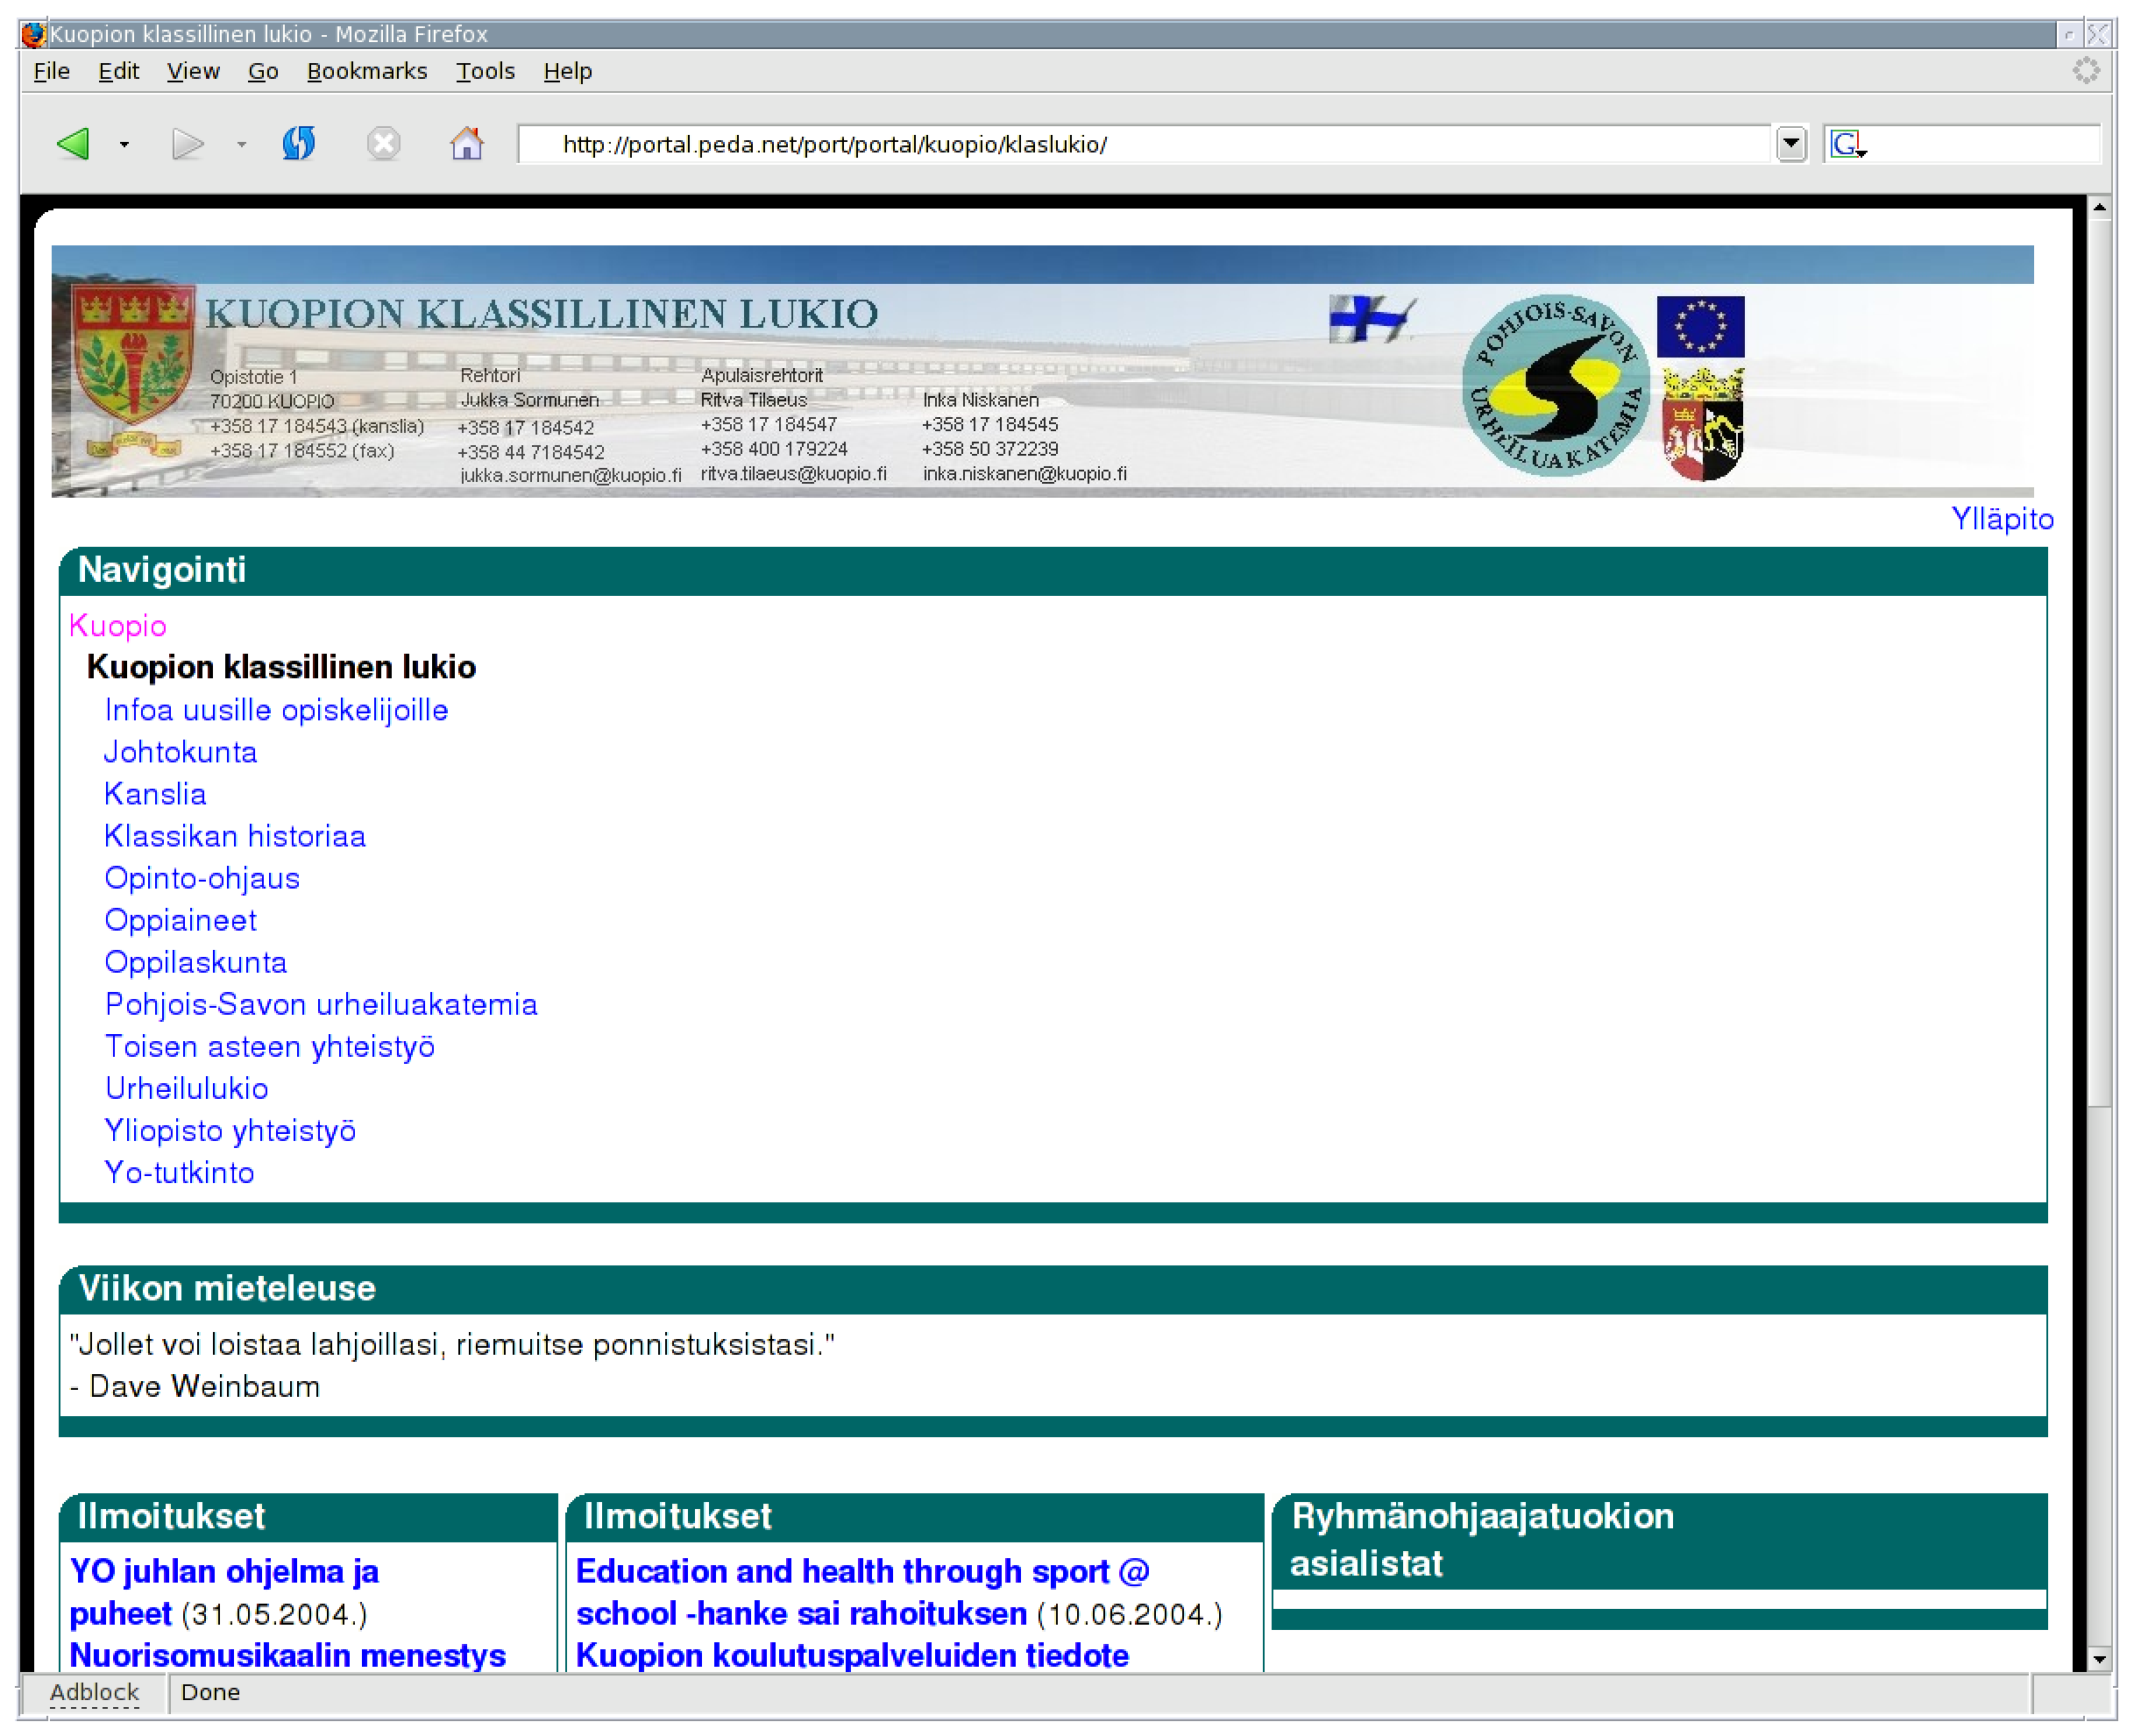
\includegraphics[width=12cm]{kuvat/lukio1}
\caption{Kuopion Klassillisen lukion ver�j�}
\label{fig:veraja1}
\end{kuva}

Portaali eli \emph{Verkkover�j�} kehitettiin alunperin vuonna 2001
nimenomaan www"-portaaliksi, jonne opettajat voisivat luoda linkkej�
opetukseen liittyv��n materiaaliin. Sovellusta kehitett�ess� p��tettiin
lis�t� mahdollisuus my�s pienimuotoiseen muun sis�ll�n tuottamiseen ja
sivun taittoon. T�ll�iselle ty�kalulle oli tarvetta, koska www"-sivujen
yll�pito k�sin oli liian vaikeaa tavalliselle opettajalle. Kaikilla
kouluilla ei ollut tuohon aikaa www"-sivuja ollenkaan ja useimmissa
tapauksissa www"-sivujen yll�pidon hallitsi vain yksi henkil�, jonka
kautta kaikki muutokset sivuihin piti tehd�. Opettajan oli vaikea
asettaa yksitt�iseen koulun kurssiin liittyv� s�hk�inen materiaali
saataville.

My�hemmin ty�kalun kehittyess� tavoitteena oli tukea my�s yleisemmin
www"-sivujen tuotantoa -- esimerkiksi koulun kotisivujen muodossa.
Usein koulun selaimessa n�kyikin oletuksena ensimm�isen� paikallisen
internet"-operaattorin etusivu, koska koululla ei ollut omia
kotisivuja. T�m� palveli huonosti itse opetusteht�v��. Verkkover�j�n
yhteydess� www"-sivulla tarkoitetaan muutakin kuin pelk�n tekstin ja
kuvien julkaisemista. Lis�ksi voidaan k�ytt�� esimerkiksi
verkkokeskusteluja tai yhteist� kalenteria. Sivu kootaan ns.
moduuleista, joita ladotaan k�ytt�liittym��n tarjolla oleviin
layout"-malleihin. Ideana on, ett� yksi moduuli tarjoaa yhden
toiminnon: esimerkiksi kuva"-moduulilla voi sivulle liitt�� kuvan ja
kuvatekstin. Kuvassa \ref{fig:veraja1} on esimerkkin� Kuopion
Klassillisen lukion ver�j� alkuper�isen Ver�j�n k�ytt�liittym�n kautta
tarkasteltuna.

Verkkover�j� oli viimeinen Peda.netiss� Perl"-ohjelmointikielell�
toteutettu ja julkaistu sovellus. Verkkover�j� toimi MySQL"-tietokannan
p��ll� ja nykyisin k�yt�ss� oleva, Juha Lahden PHP"-ohjelmointikielell�
vuonna 2004 kirjoittama versio, k�ytt��kin edelleen olennaisesti samaa
tietokantaa.

\subsection{Portal2"-prototyyppi}

Portaalista eli verkkover�j�st� ryhdyttiin kehitt�m��n toista versiota
vuonna 2002. Kehitys eteni t�ysin toimivan sovelluksen toteutukseen
asti. Uusi versio tarjosi mahdollisuuden vaikuttaa portaalin ulkon�k��n
huomattavasti enemm�n ja merkitt�v�n� toiminnallisena uutuutena
moduuleita voitiin tarjota julkisesti tarjolle muiden opettajien
ver�jiin. T�ll�in esimerkiksi yksitt�isen opettajan tuottamaa
matematiikan aineistoa voitaisiin k�ytt�� toisen koulun matematiikan
kurssilla, integroituna muuhun sen kurssin k�ytt�m��n materiaaliin.

%\begin{kuva}
%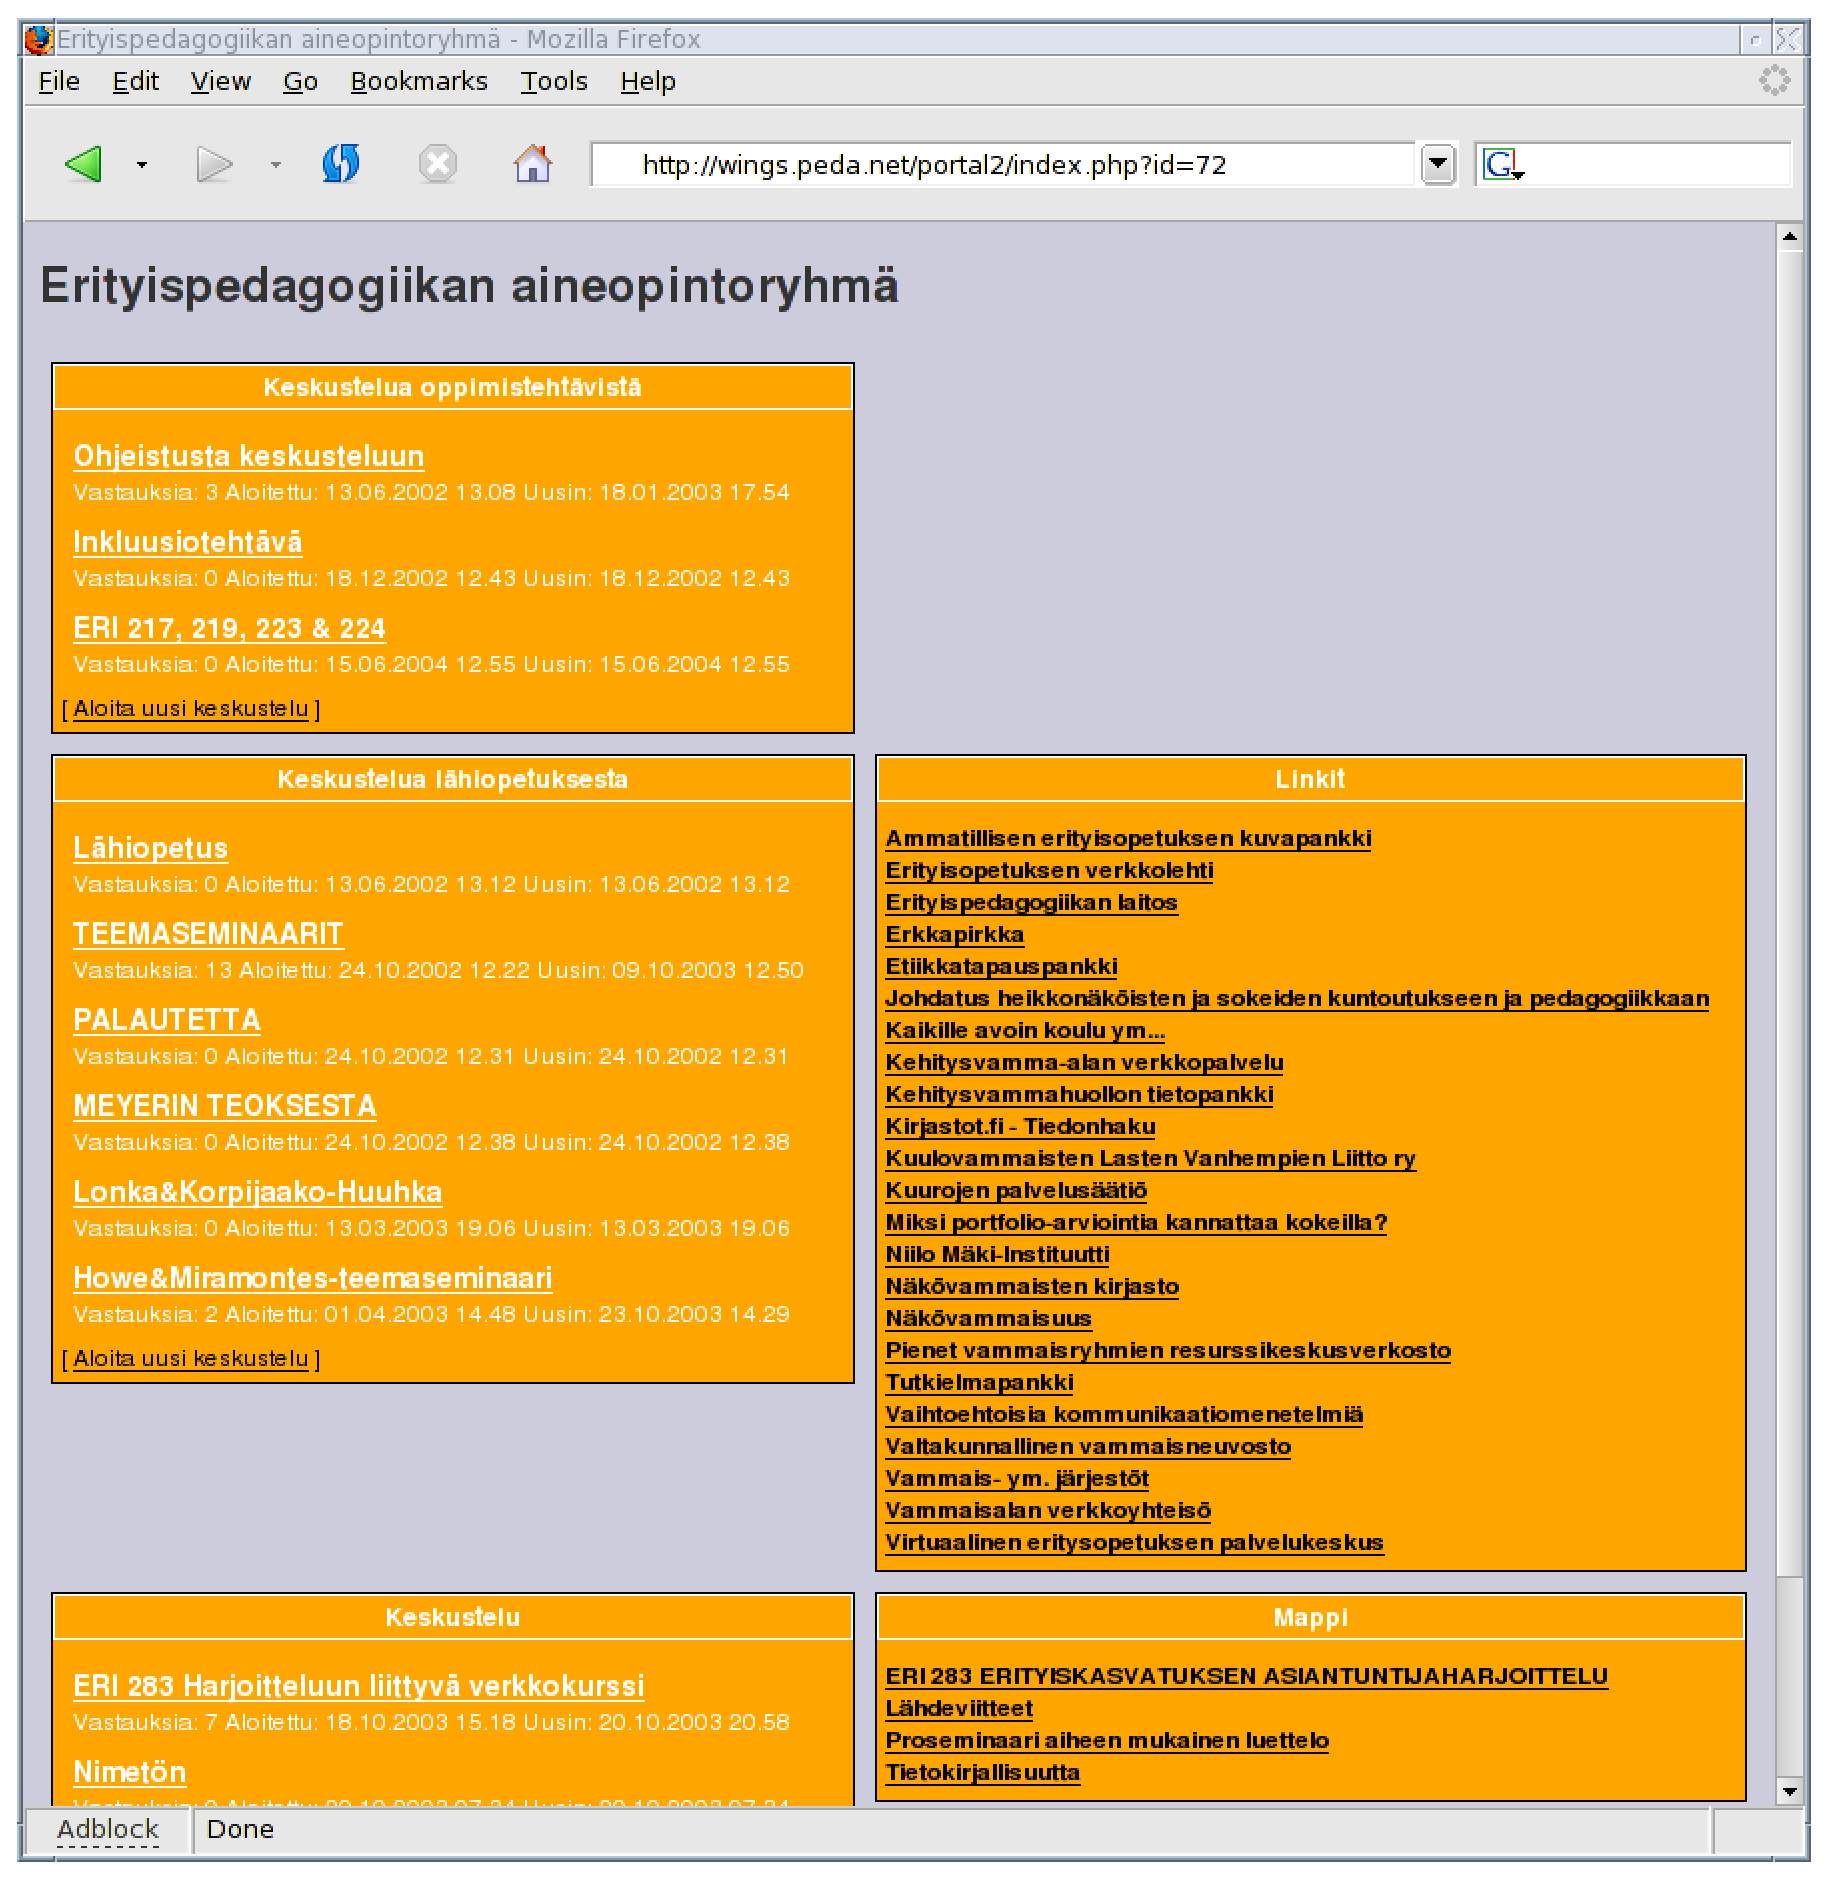
\includegraphics[width=10cm]{kuvat/portal2}
%\caption{Kuva Portal2"-prototyypist�}
%\label{fig:portal2}
%\end{kuva}

\begin{kuva}
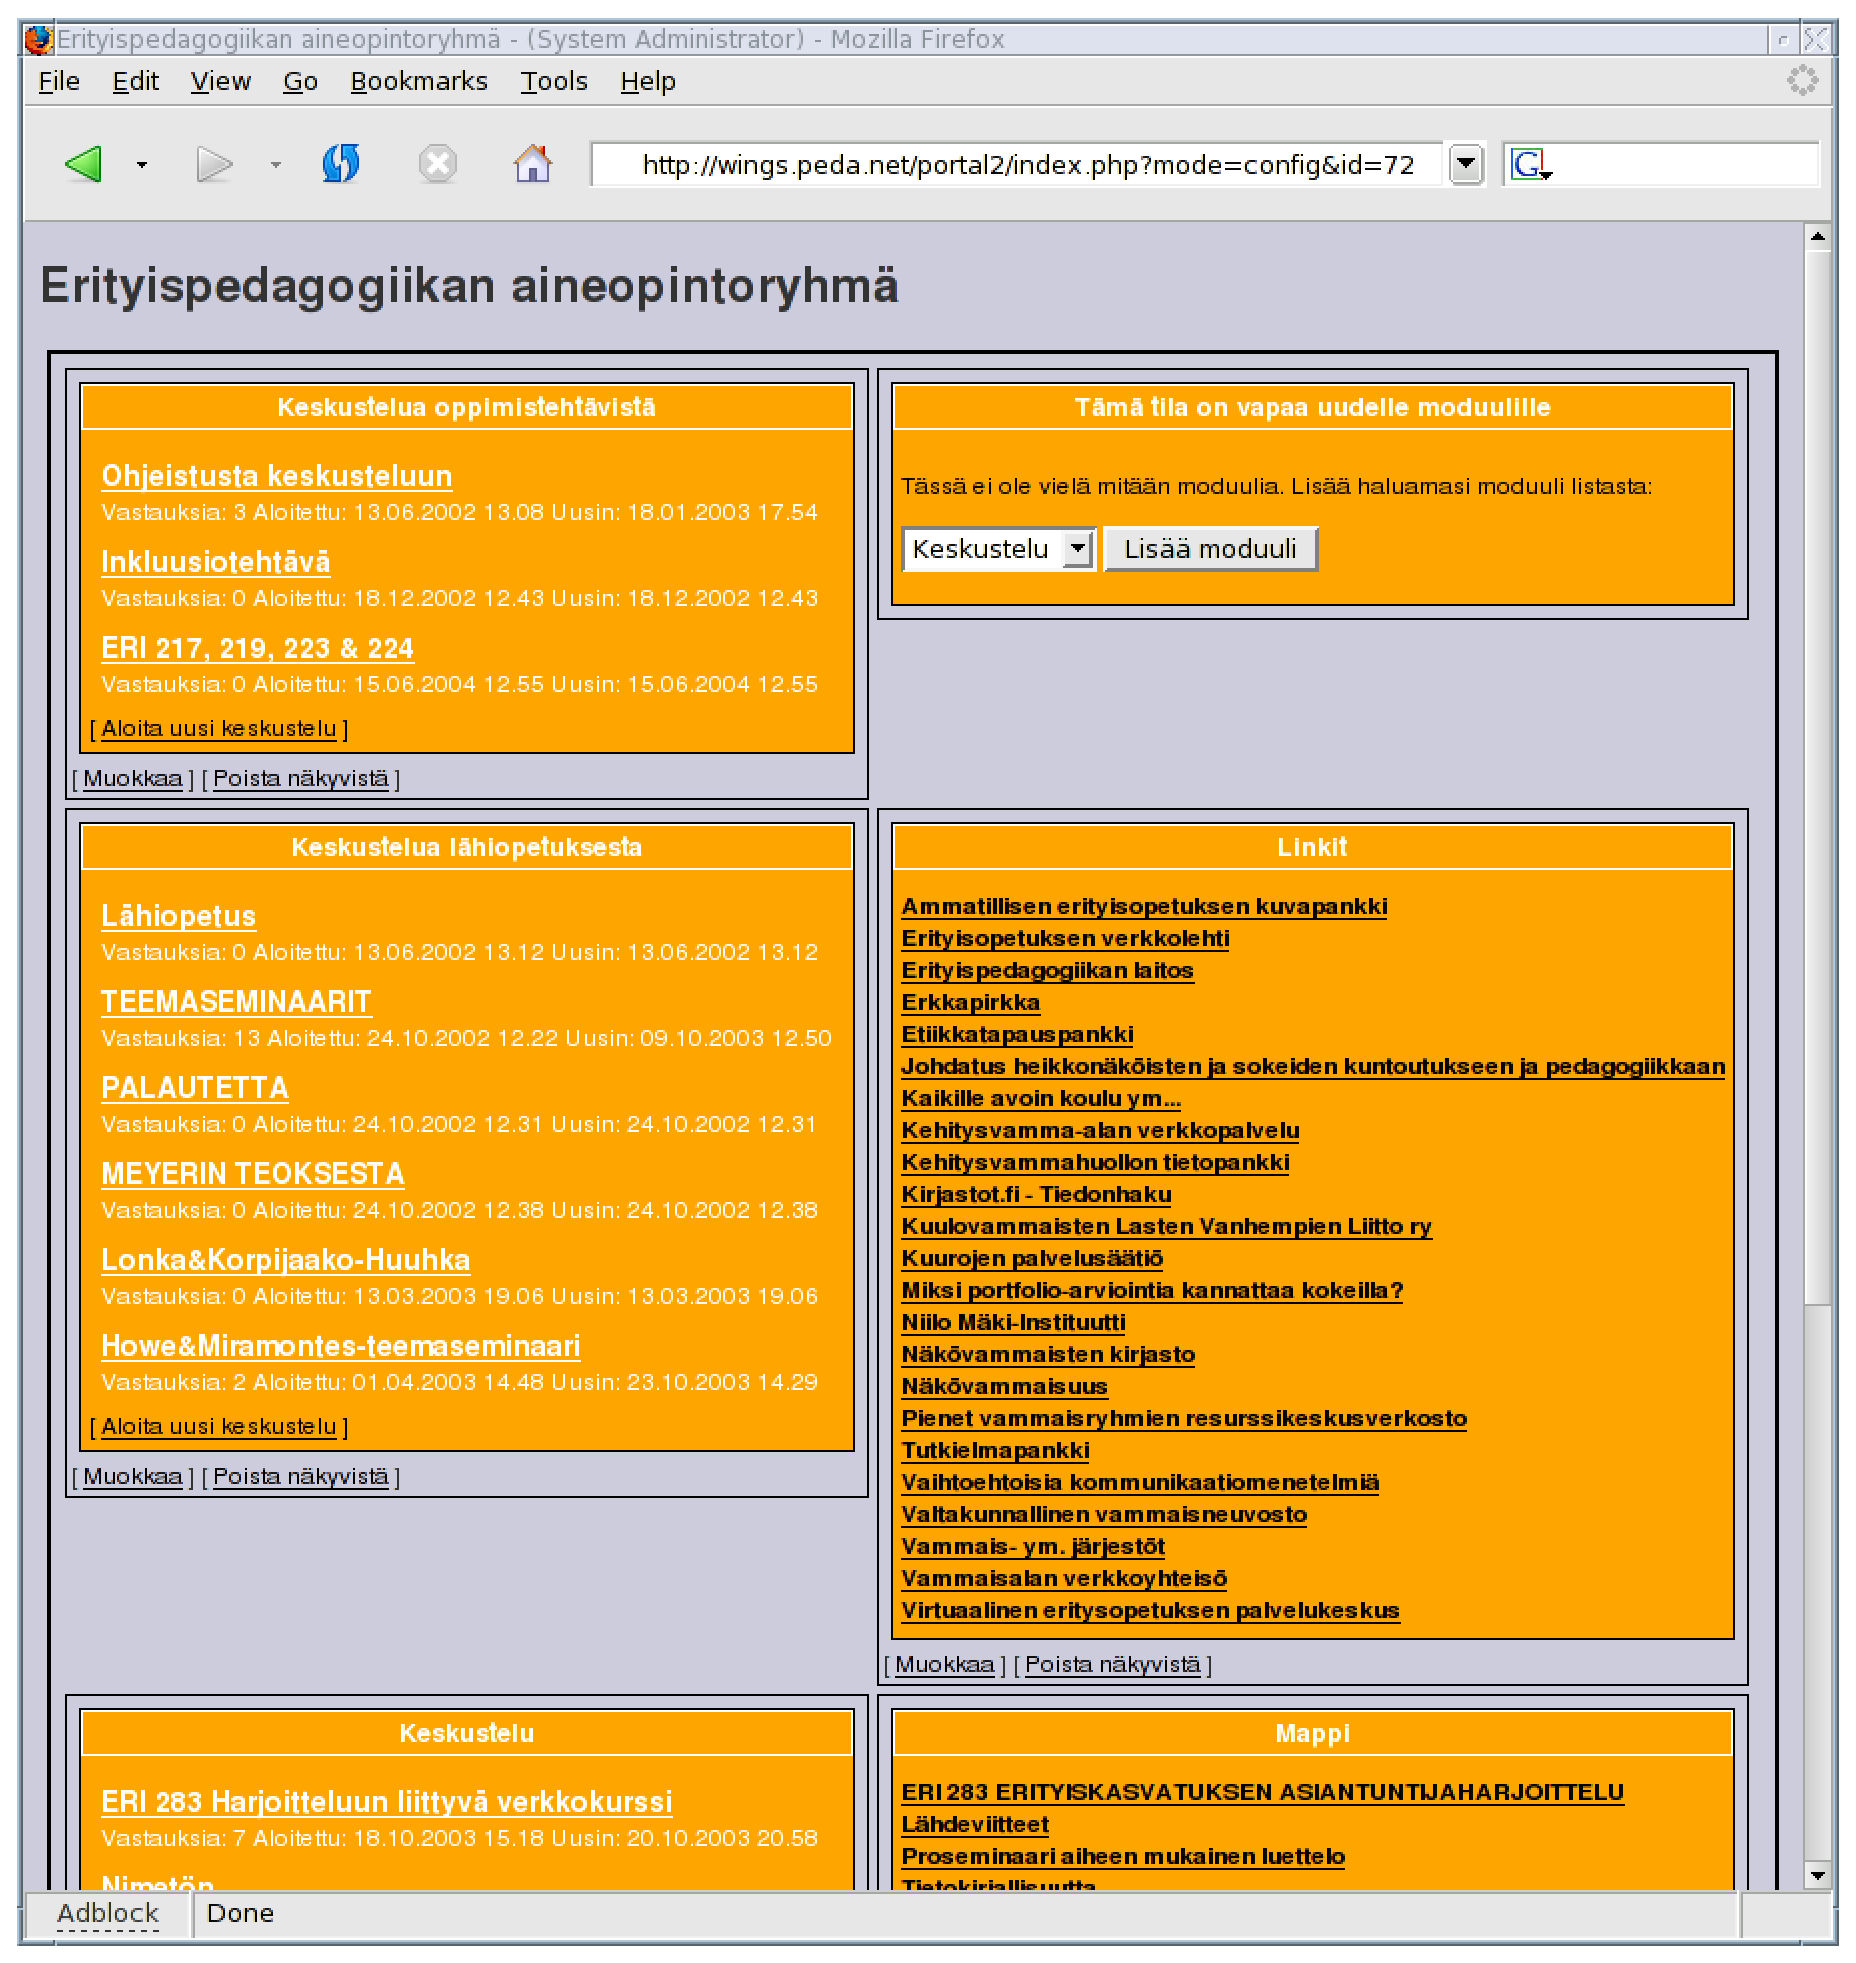
\includegraphics[width=10cm]{kuvat/portal22}
\caption{Kuva Portal2"-prototyypin yll�piton�kym�st�}
\label{fig:portal22}
\end{kuva}

Ohjelma tehtiin uuden ep�yhteensopivan tietokantarakenteen p��lle,
mutta my�hemmin p��dyttiin tulokseen, ett� uuden version tarjoamat
uudet toiminnot eiv�t tuoneet riitt�v�sti etuja, jotta vanhan version
k�ytt�jien olisi kannattanut siirty� k�ytt�m��n uutta versiota.
Merkitt�v�n� erona t�ss� versiossa oli erotettu moduulien luonti,
poistaminen ja muokkaus erilliseksi toiminnoksi sivun asettelusta.
Koulujen opettajien silloinen tietotaito ei riitt�nyt hallitsemaan
sis�ll�n ja ulkon��n erottelua tai sitten t�m�n toiminnallisuuden
esitt�minen www"-selaimen ehdoilla ep�onnistui. Todettiin, ett�
koulujen opettajille uusi versio oli vaikeak�ytt�isempi kuin edellinen
versio.

Kahden rinnakkaisen, miltei samaan k�ytt��n tarkoitetun
sovelluksen yll�pit�miseen ei haluttu ryhty�. My�s Portal2 tehtiin
viel� Perl"-ohjelmointikielell� MySQL"-tietokannan p��lle. Puutteistaan
huolimatta Portal2 on ollut pienimuotoisessa k�yt�ss� muuttamattomana ja sit� k�ytt�en on j�rjestetty Avoimen Yliopiston kursseja
viel� talvella 2004.

Juha Lahti kirjoitti Ver�j�st� kev��ll� 2004 julkaistun kolmannen
version; se sis�lsi suuren samoista toiminnoista kuin Portal2, tosin
moduulien jakamista ei ole ainakaan viel� toteutettu. Samoin
k�ytt�liittym�n logiikka kopioitiin pienin muutoksin ensimm�isest�,
toimivaksi havaitusta versiosta. Kolmas versio p��tettiin my�s kehitt��
t�ysin yhteensopivaksi ensimm�isen kanssa, jolloin kaikkien vanhojen
portaalien sis�lt� olisi v�litt�m�sti k�ytett�viss� my�s uuden
k�ytt�liittym�n kautta. Siirtym�vaiheessa, joka kesti vuoden 2004
alusta saman vuoden syksyyn, portaalien k�ytt� ja yll�pito onnistui
molempien k�ytt�liittymien kautta. Vanha k�ytt�liittym� poistettiin
k�yt�st�, jotta uusia ominaisuuksia lis�tt�ess� ei tarvitsee huomioida
kuin uusin k�ytt�liittym�.

\begin{kuva}
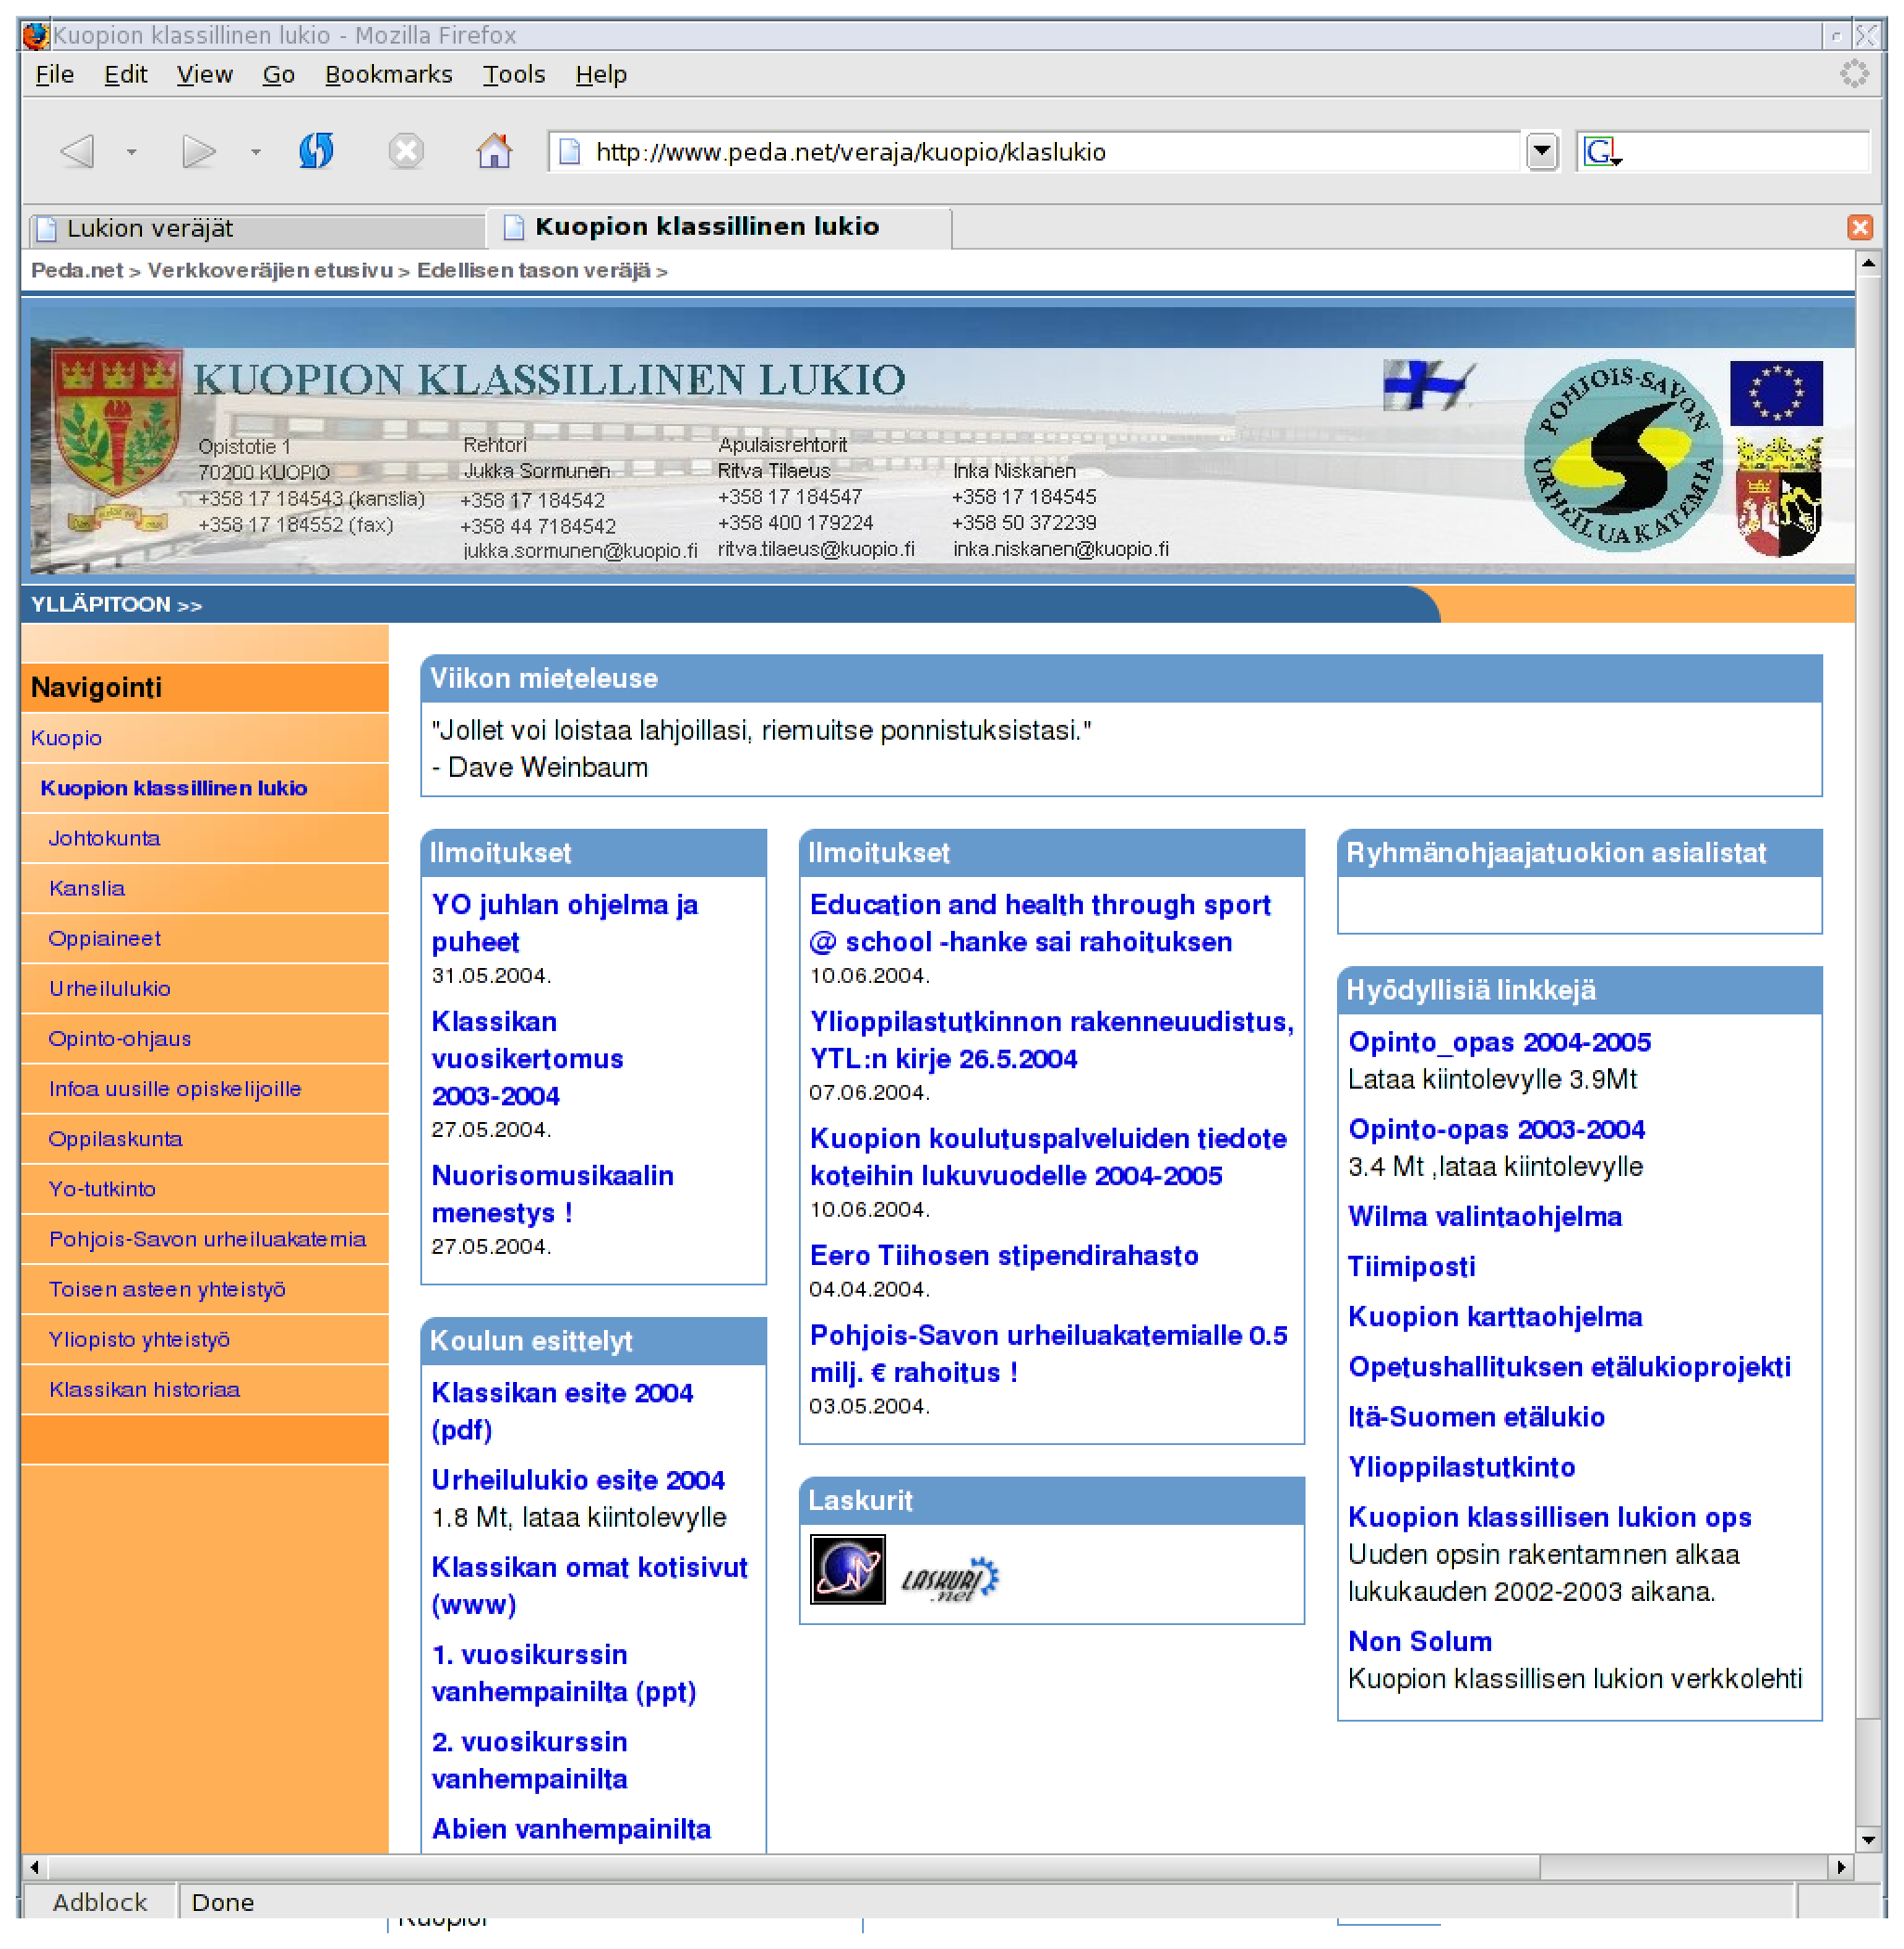
\includegraphics[width=10cm]{kuvat/lukio2}
\caption{Kuopion Klassillisen lukion ver�j� (uusi k�ytt�liittym�)}
\label{fig:veraja2}
\end{kuva}


Kev��ll� 2004 verkkover�ji� oli k�yt�ss� noin 13000. Suuren
k�ytt�j�m��r�n ansiosta saamme paljoin toiveita uusien toimintojen
suhteen; tulevaisuudessa kehityspaineita on sivukokonaisuuksien
yll�pidon kehitt�miseen ja materiaalin jakamisen automatisointiin.
T�ll� hetkell� jokainen verkkover�j� on itsen�inen kokonaisuus. Kuvassa
\ref{fig:veraja2} on Kuopion Klassillisen lukion ver�j� uuden
k�ytt�liittym�n kautta katseltuna -- kyseess� on siis sama ver�j� kuin
kuvassa \ref{fig:veraja1}.

Ver�j�n vuoden 2004 versio oli Peda.netin ensimm�inen kokonaan uusittu
ty�kalu, joka oli t�ysin yhteensopiva entisen version sis�ll�n kanssa
ja sit� pystyi k�ytt�m��n samanaikaisesti vanhan version kanssa.
K�ytt�jilt� tuli t�st� mahdollisuudesta paljon positiivista palautetta,
mutta t�ydellisen yhteensopivuuden vuoksi sovelluksen kehitt�minen oli
vaikeampaa kuin ep�yhteensopivan version kehitt�minen olisi ollut.

\subsection{YALE2"-sovellus}

YALE2 eli Yet Another Learning Environment 2 on kokonaan
PHP"-ohjelmointikielell� vuonna 2003 uudelleenkirjoittamani versio Juha
Lahden tekem�st� YALE"-prototyypist�. YALE2 on selaink�ytt�inen
oppimisymp�rist� yksitt�isen koulun k�ytt��n. YALE2 tarjosi
suljettujen, oppilaiden k�ytt��n luotujen kurssien luomisen ja
yll�pidon lis�ksi julkaisumahdollisuuden kirjasto"-nimisen ominaisuuden
muodossa.

YALE2 on t�t� kirjoittaessa edelleen pienimuotoisessa testik�yt�ss�,
mutta sit� ei tulla virallisesti ottamaan k�ytt��n miss��n vaiheessa.
Sovellus poistetaan k�yt�st� vuoden 2004 loppuun menness�. YALE2 oli
loogisesti Oppimapin esiaste, jossa ei ollut versionhallintaa ja
oikeuksien hallinta oli huomattavasti rajoittuneempaa. Lis�ksi
k�ytt�liittym�n rakenteessa oli joitakin k�ytett�vyysongelmia. Uuden
version kehitt�miseen p��dyttiin, koska versionhallinnan ja
kehittyneemm�n oikeuksien hallinnan liitt�minen t�h�n versioon
arvioitiin ty�l��mm�ksi kuin kokonaan uuden j�rjestelm�n kehitt�minen.

%\begin{kuva}
%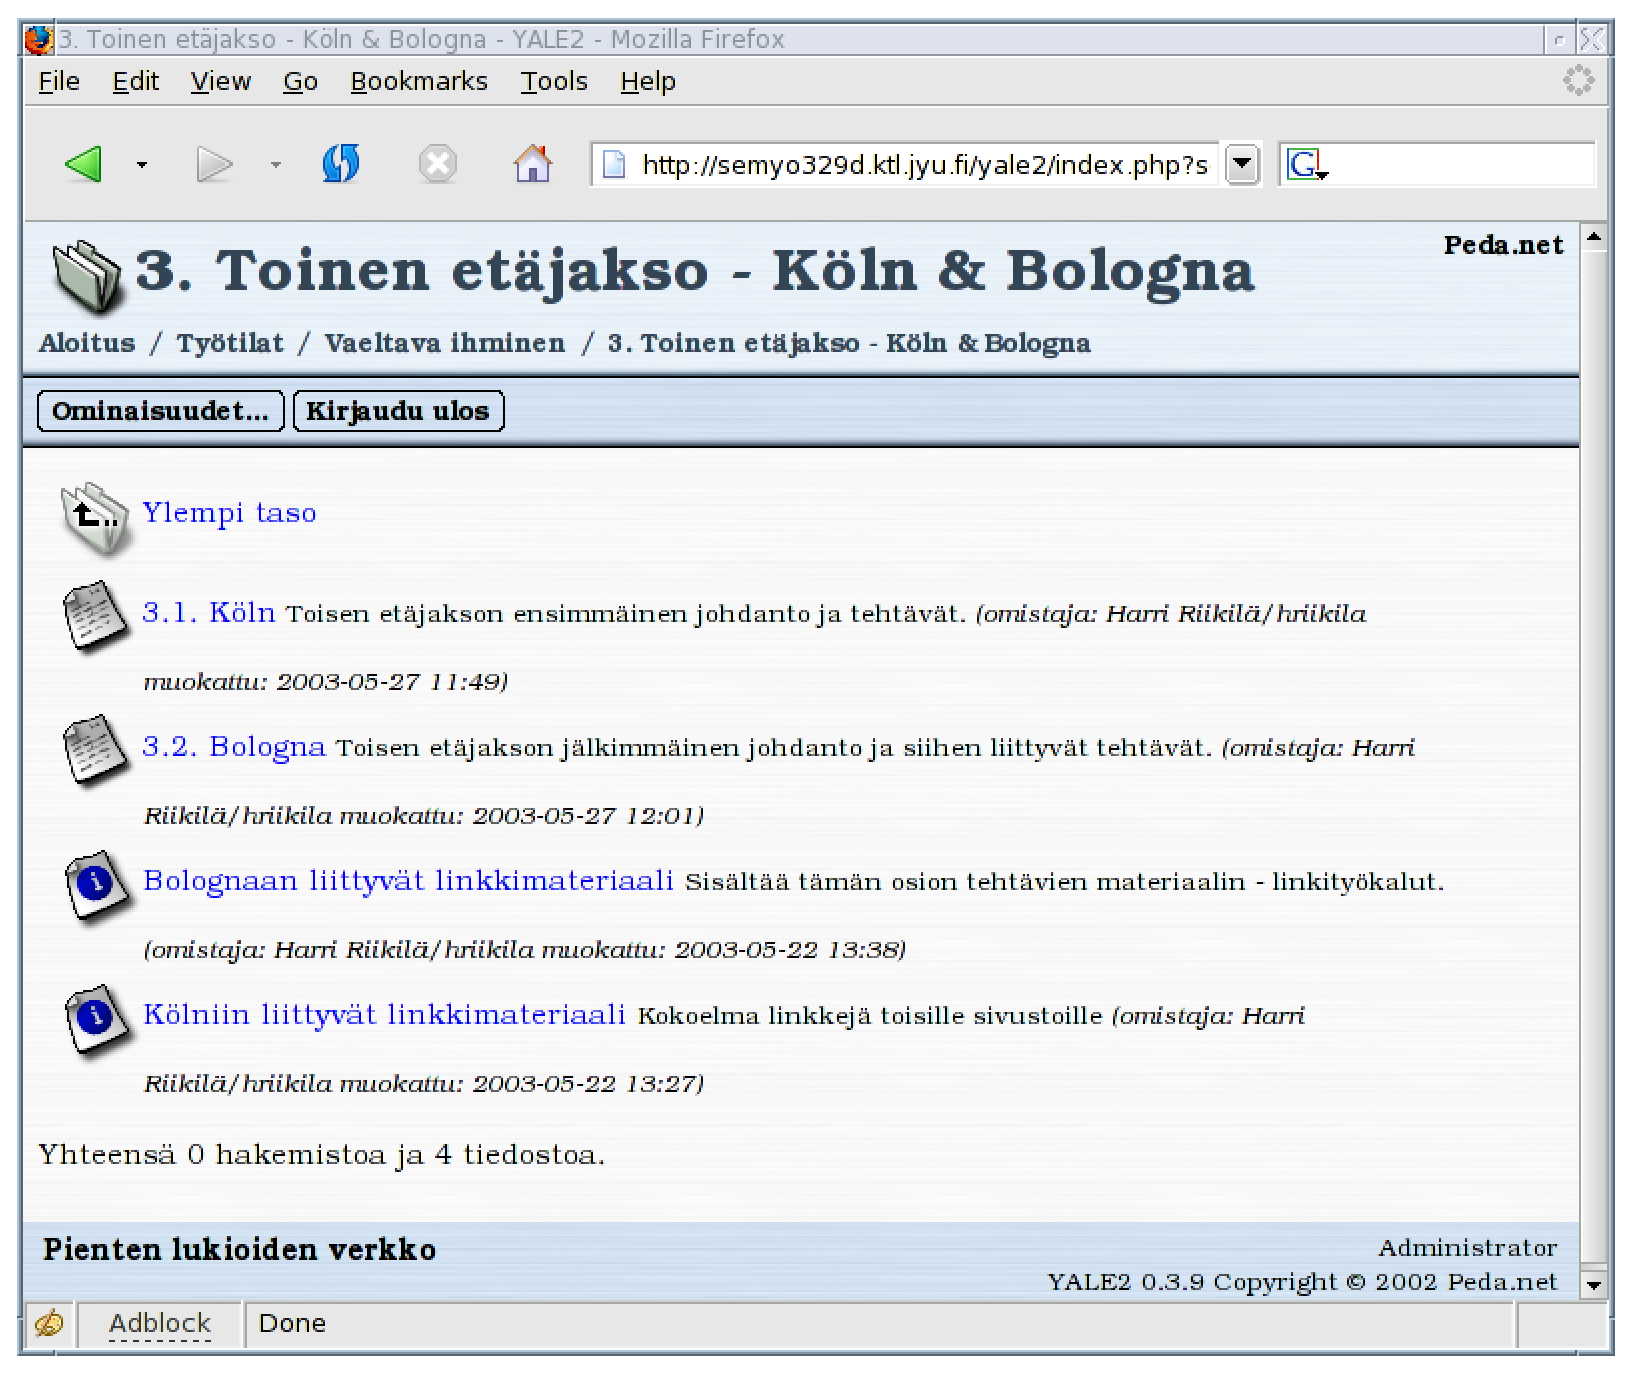
\includegraphics[width=10cm]{kuvat/yale21}
%\caption{YALE2: yksitt�isen kurssin n�kym�}
%\label{fig:yale21}
%\end{kuva}

\begin{kuva}
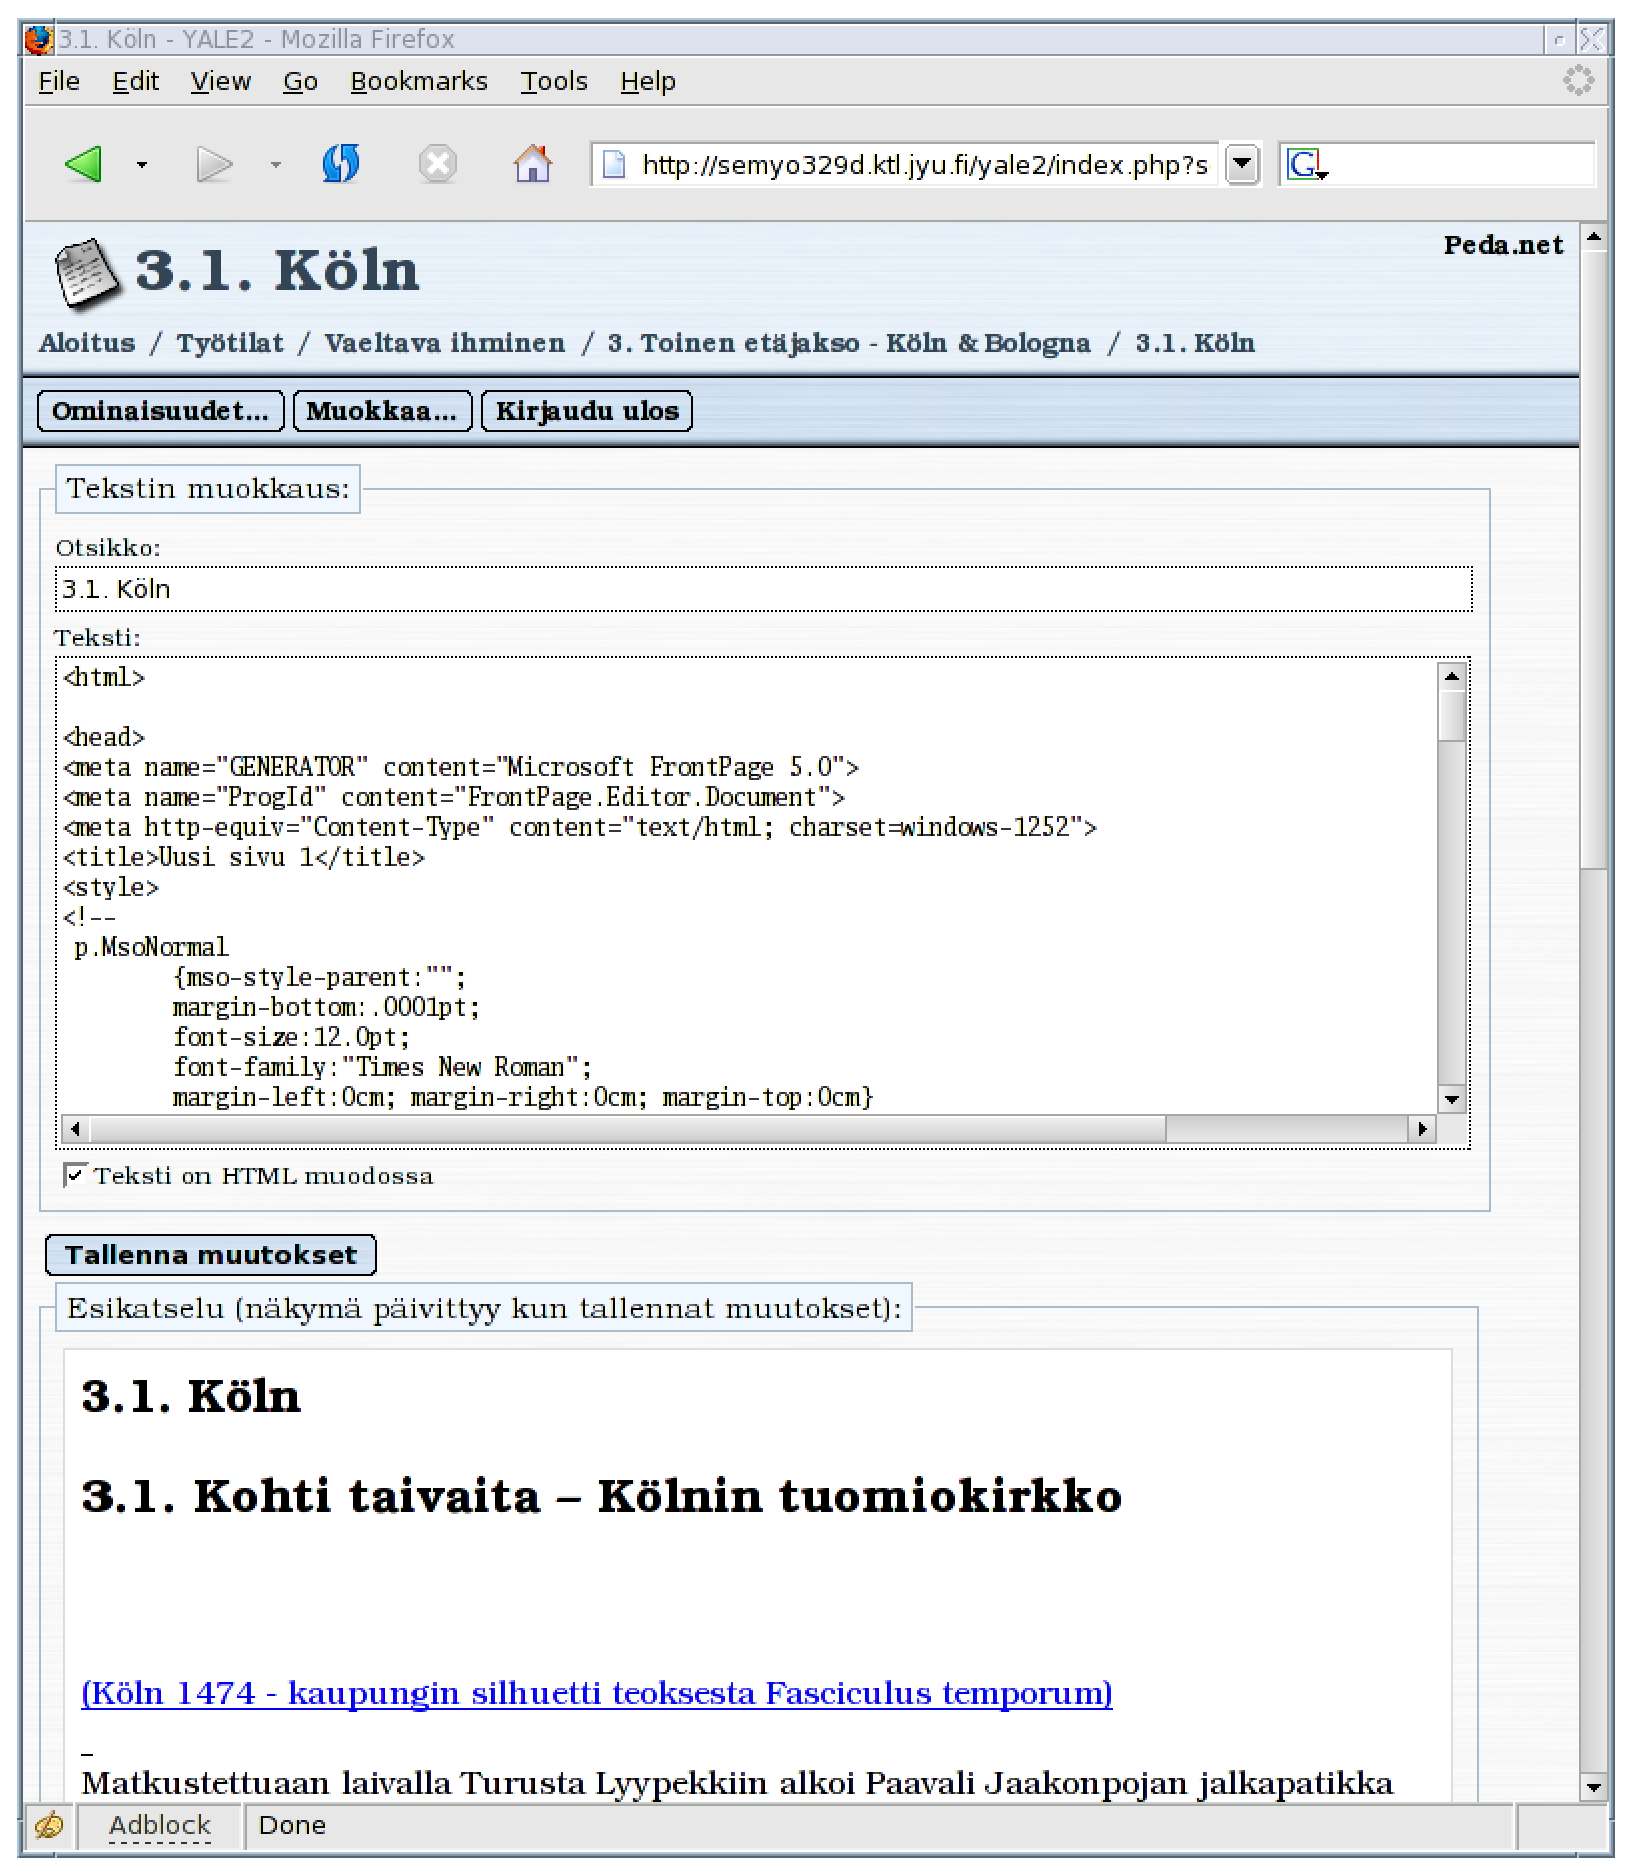
\includegraphics[width=10cm]{kuvat/yale22}
\caption{YALE2: esimerkki kurssin materiaalin muokkaamisesta}
\label{fig:yale22}
\end{kuva}

\subsection{Oppimappi}
\label{pedanet-oppimappi}

Peda.net Oppimappi on nykyinen kehitysprojektini, joka
tarjoaa yksitt�isen koulun kaikille kursseille riitt�v�n
oppimisymp�rist�n.T�m� sovellus ei tue kurssien j�rjest�mist� usean eri
oppilaitoksen kesken, vaan se on suunniteltu yksitt�isen koulun
tarpeita varten. Rajaukseen p��dyttiin, koska ohjelman toteuttamisen
ty�m��r�n arvioitiin kasvavan liian suureksi nykyisiin resursseihin
verrattuna. Sovellusta on kehitetty kes�st� 2003 alkaen ja se
julkaistiin syksyll� 2004. Kuten selaink�ytt�isten sovellusten
tapauksessa yleens�, julkaisu ei tarkoita sovelluksen kehityksen
lopettamista t�ss�k��n tapauksessa. Uusia ominaisuuksia tullaan
lis��m��n julkaisun j�lkeen k�ytt�jien toiveiden mukaan. Samoin
k�ytt�liittym� k��nnet��n eri kielille; tuetut kielet sis�lt�v�t
ainakin suomen, ruotsin, englannin, saksan ja saamen.

\begin{kuva}
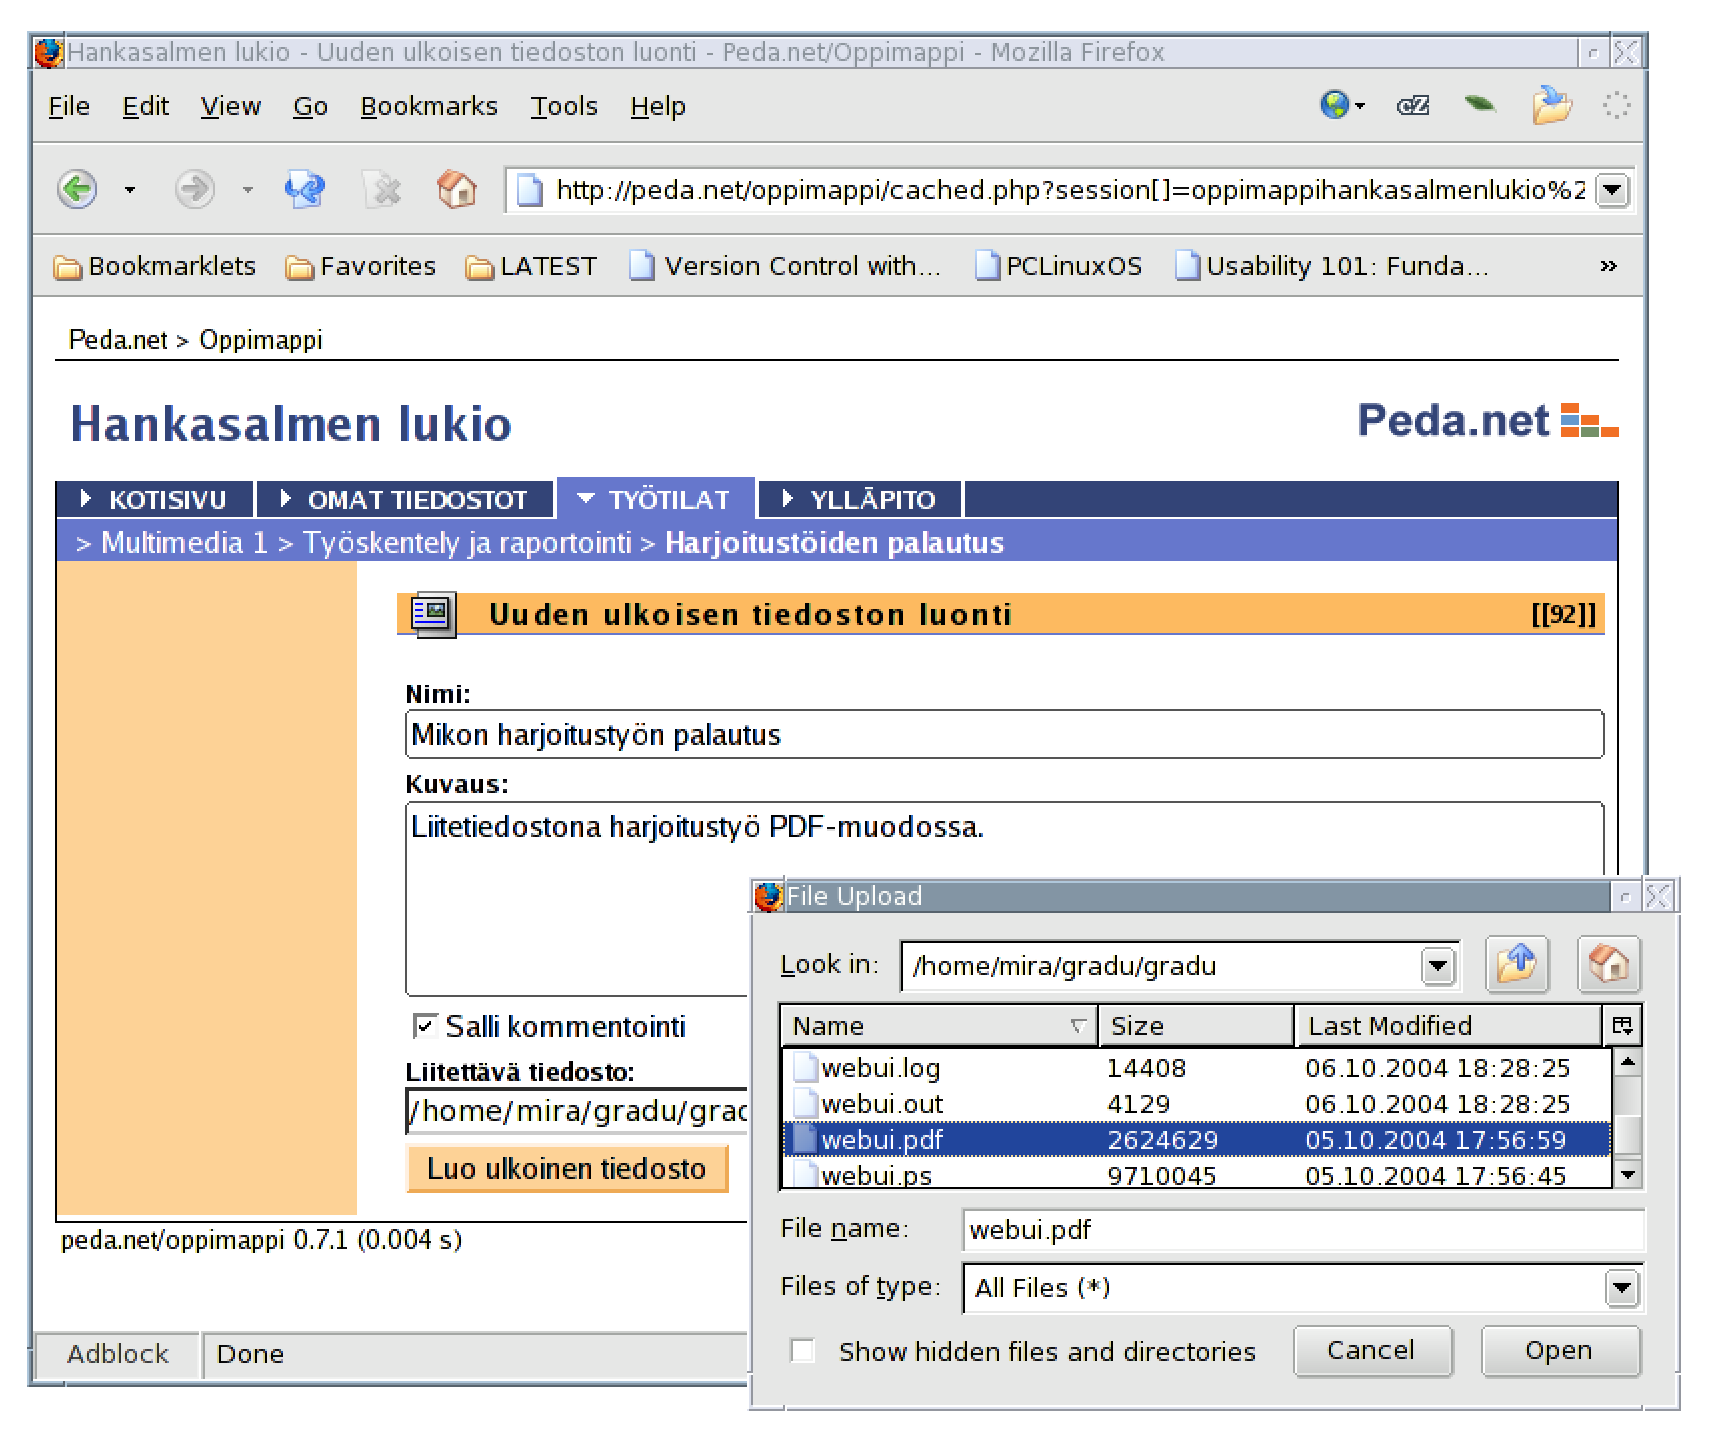
\includegraphics[width=10cm]{kuvat/oppimappi}
\caption{Esimerkki Oppimapin k�ytt�liittym�st�}
\label{fig:oppimappi}
\end{kuva}

Yll�pit�j�n kannalta merkitt�vi� ominaisuuksia ovat k�ytt�jien hallinta
monitasoisten ryhmien kautta, kurssien ja kurssimateriaalien oikeuksien
m��rittely luku- ja kirjoitusoikeuksien avulla ja versionhallinta sek�
kaiken materiaalin vapaa linkitt�minen mihin tahansa j�rjestelm�n
sis�ll�. Loogisella tasolla Oppimapissa yll�pidet��n kaksisuuntaista
hierarkiaa, joka muodostuu erilaisista dokumenttityypeist� tai
moduuleista. Eri dokumenttityyppej� ovat muun muassa kansiot,
tiedostot, keskustelut ja ty�tilat. Jokainen moduuli voi sis�lt�� muita
moduuleita ja jokainen moduuli voi n�ky� monen eri moduulin sis�ll�.
Tietokanta mahdollistaa jopa moduulin n�kymisen itsens� sis�ll�. Osaa
toiminnoista on rajoitettu k�ytt�j�n toimien helpottamiseksi.
Esimerkiksi k�ytt�liittym� ei tarjoa mahdollisuutta luoda ty�tiloja
keskustelun sis�lle (tosin olemassaolevaan ty�tilaan voi viitava keskustelussa, jolloin j�rjestelm� tarjoaa polun kulkea kyseiseen ty�tilaan keskustelun kautta).

%Peda.net on t�ll� hetkell� Suomen johtava oppimisymp�rist�jen
%toimittaja k�ytt�j�m��r�ss� mitattuna.

\chapter{Peda.net Oppimapin k�ytett�vyyden arviointia}

Oppimapin k�ytt�liittym�n p��osat muodostuvat navigointipalkista,
toimintovalikosta ja sis�lt�alueesta. Kuvassa
\ref{fig:oppimappi-kotisivu} on esitetty Oppimapin kotisivu"-n�kym�
yll�pit�j�n oikeuksilla. T�m� on Oppimapin aloitussivu
sis��nkirjautumisen j�lkeen. Yl�reunassa n�kyy Oppimapin otsikko (t�ss�
esimerkiss� ``Hankasalmen lukio'') ja linkit eri alueille Oppimapin
sis�ll�: kotisivu, omat tiedostot, ty�tilat ja yll�pito. Vasemman
reunan palkissa on aina sen hetkist� sis�lt�� koskevat toiminnot, t�ss�
tapauksessa  vain ''palauta poistetut kohteet'', joka palauttaisi
sis�lt�listaukseen ne dokumentit, ty�tilat ja kansiot, jotka k�ytt�j�
on aikaisemmin itse poistanut. Itse sis�lt�alue muodostuu t�ll� sivulla
erilaisista objekteista, joilla jokaisella on ikoni, nimi, kuvaus ja
toimintoja. Nimest� n�p�ytt�m�ll� p��see k�ytt�m��n objektia ja
objektin per�ss� olevaa toimintoa k�ytt�m�ll� sen ominaisuuksiin voi
vaikuttaa.

\begin{kuva}
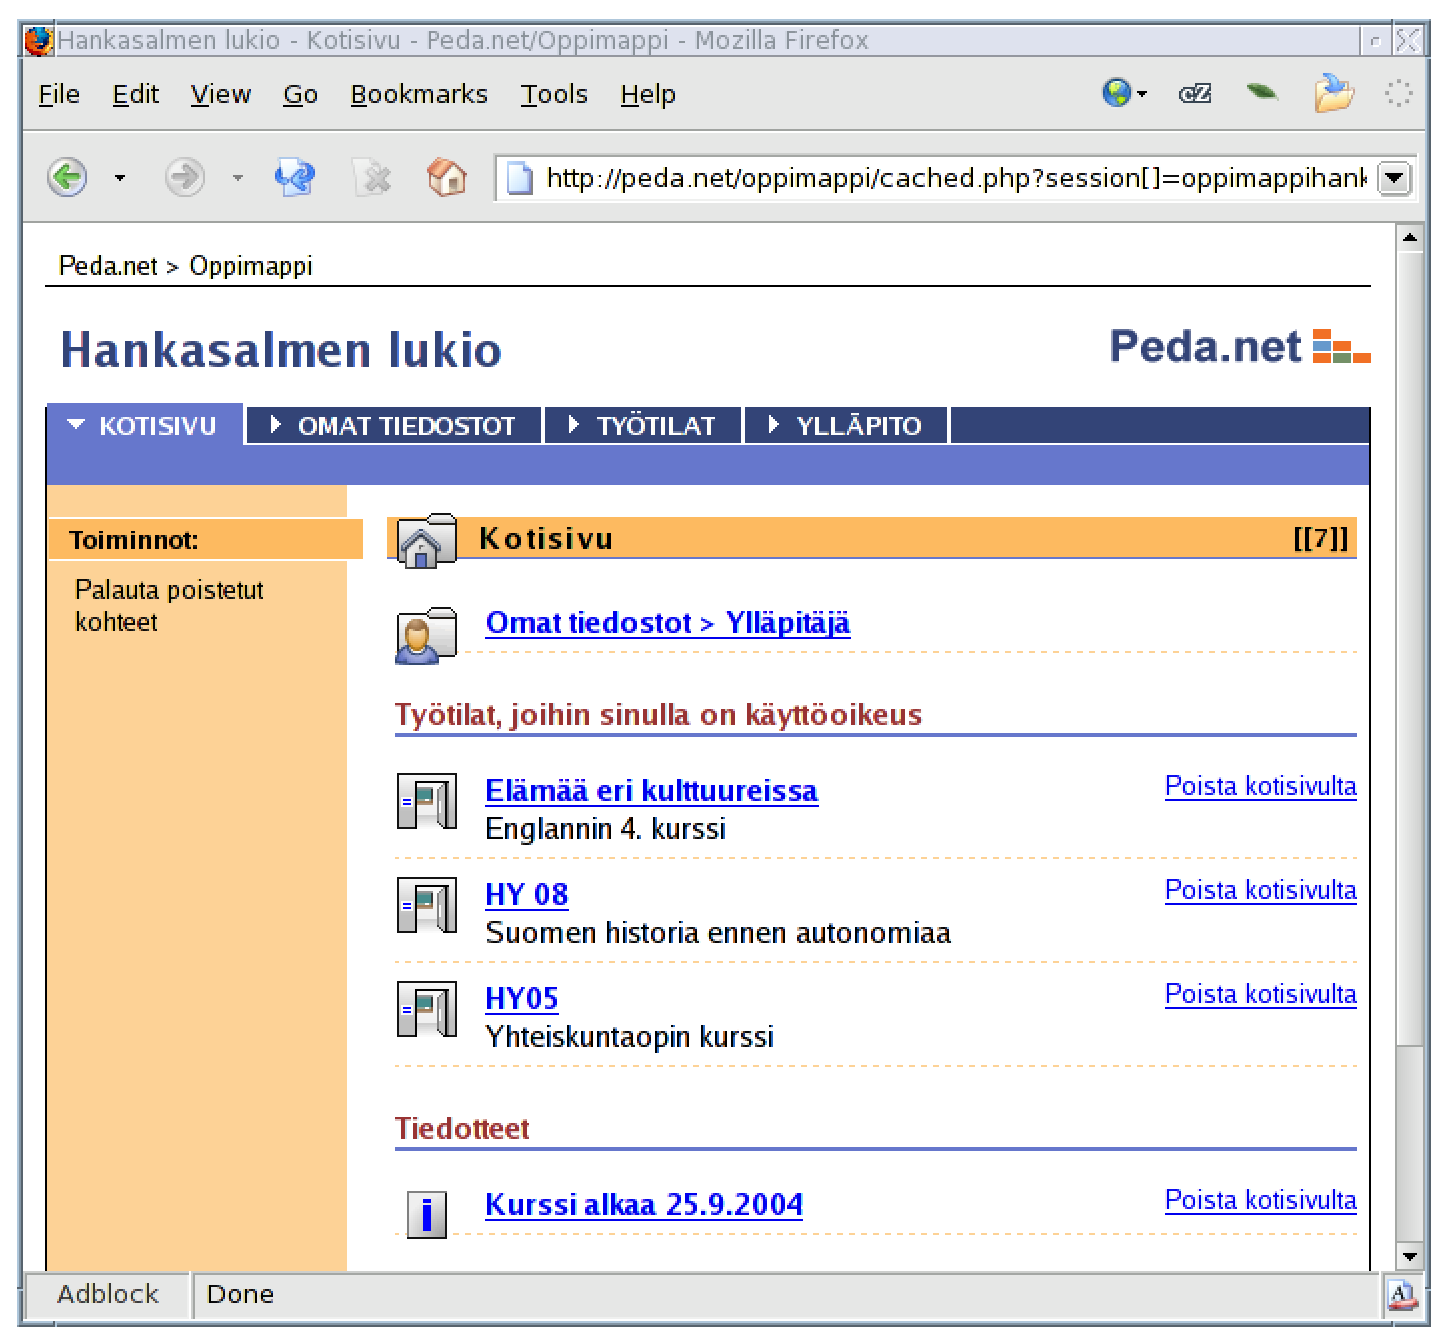
\includegraphics[width=10.0cm]{kuvat/oppimappi-kotisivu}
\caption{Oppimappi: ty�p�yt�-n�kym�}
\label{fig:oppimappi-kotisivu}
\end{kuva}

Ensimm�iseksi havaitaan, ett� t�ss�kin ymp�rist�ss� suuri osa ikkunan
pinta"-alasta menee muuhun kuin itse sis�lt��n. Navigointi ja
ymp�rist�n otsikko valtaavat suuren osan k�ytett�viss� olevasta alasta.
T�m� on seurausta valitusta tyylitiedostosta. Kuvassa
\ref{fig:oppimappi-kotisivu-nostyle} on esitetty sama n�kym� kun
CSS"-tyylisivu on selaimen asetuksista valittu pois p��lt�. T�m� n�kym�
vastaa erityisryhmien k�ytt�liittym��; esimerkiksi n�k�vammaiselle
k�ytt�j�lle tieto esitett�isiin t�m�n n�kym�n mukaisessa
j�rjestyksess�. T�ss� erityisesti nykyist� n�kyv�� koskevat toiminnot
esitet��n sis�ll�n \emph{j�lkeen} -- t�m� on t�rke��, koska yleens�
k�ytt�j� on kiinnostunut itse sis�ll�st�, ei mahdollisista
toiminnoista. Samoin kaikki sovelluksen toiminnallisuus on
k�ytett�viss� ilman kuvien lataamista tai JavaScript"-tukea.

\begin{kuva}
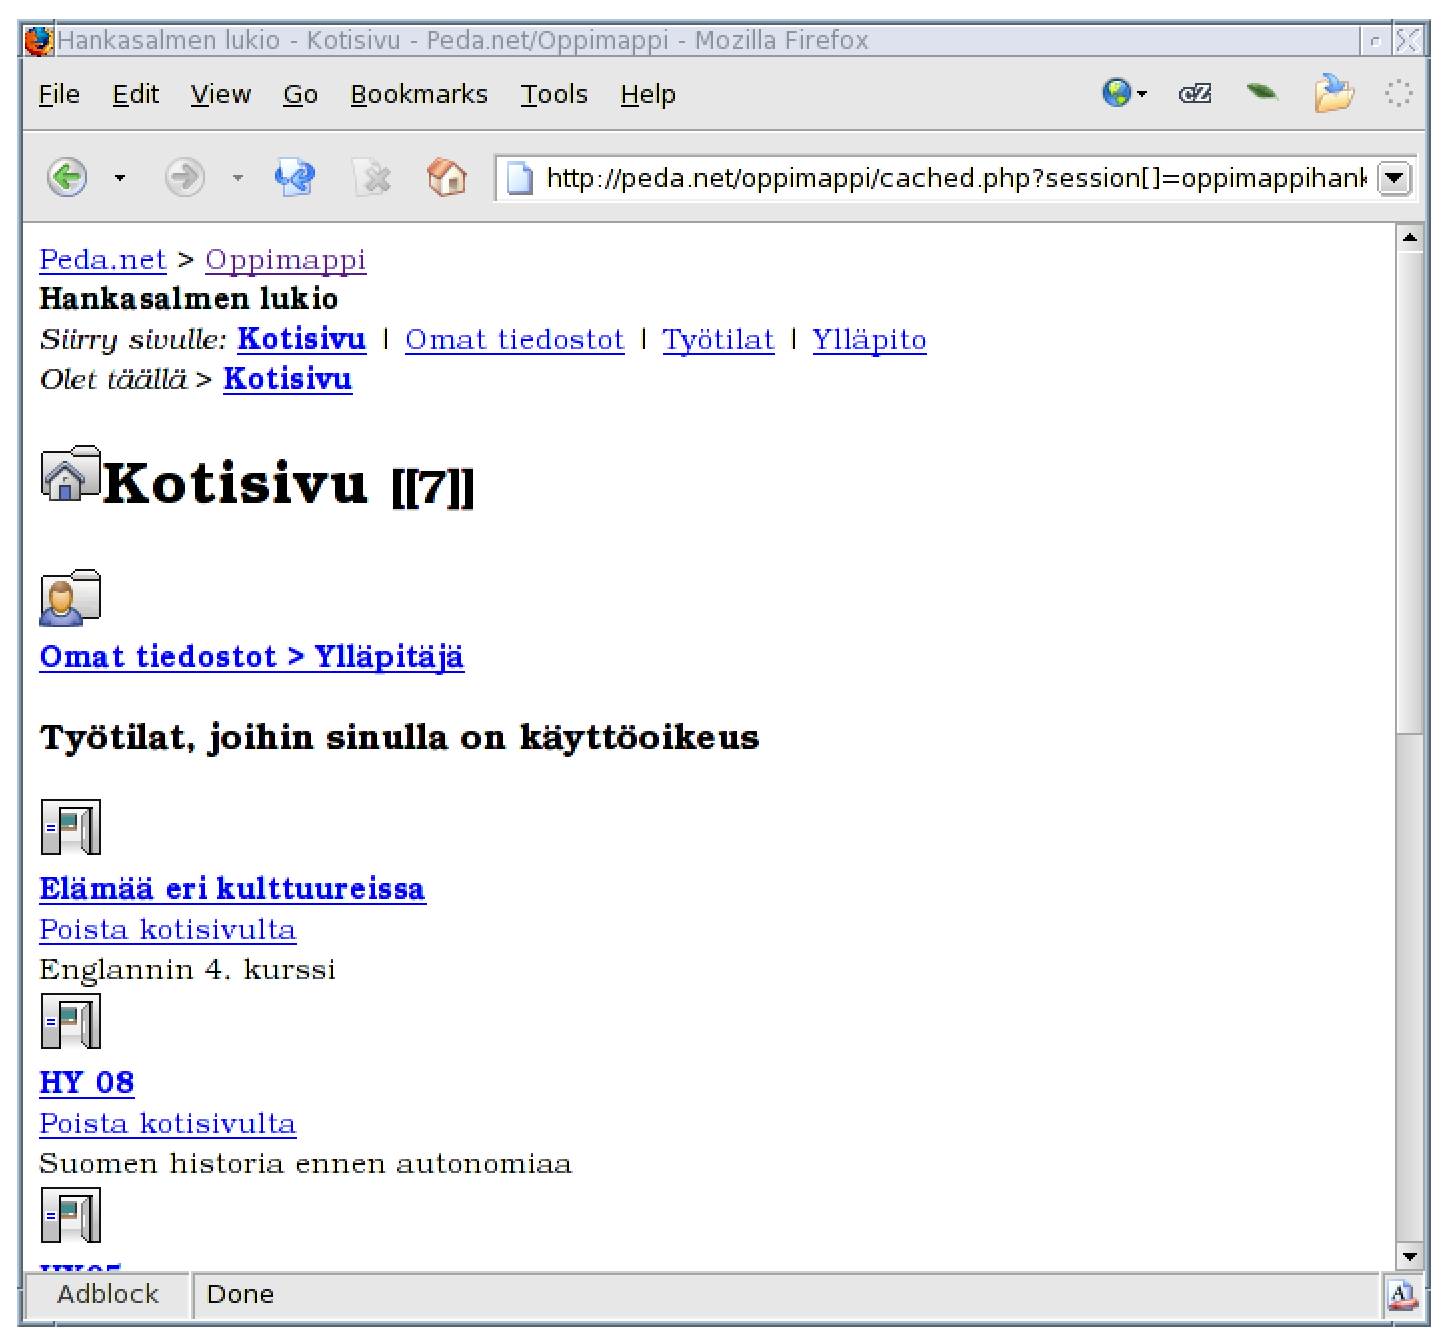
\includegraphics[width=10cm]{kuvat/oppimappi-kotisivu-nostyle}
\caption{Oppimappi: ty�p�yt�"-n�kym� ilman CSS"-tiedostoa}
\label{fig:oppimappi-kotisivu-nostyle}
\end{kuva}

T�st� n�kym�st� my�s n�hd��n, ett� kaikki sivun elementit ovat
normaaleja linkkej�. T�m�n ansiosta k�ytt�j� voi k�sitell� sivun
elementtej� aivan vastaavasti kuin tavallisenkin www"-sivun osia. Mink�
tahansa ``painikkeen'' voi lis�t� kirjanmerkkeihin tai toiminnon voi
avata toiseen ikkunaan selaimen omilla ty�kaluilla. Esimerkiksi Mozilla
Firefox "=selain avaa linkin uudessa ikkunassa, jos linkki� on painettu
keskimm�isell� hiiren painikkeella. Jos esimerkkik�ytt�j�mme avaa
``Omat tiedostot > yll�pit�j�'' "=linkin uuteen ikkunaan, saadaan kuvan
\ref{fig:oppimappi-new-window} mukainen tilanne. Olennaista t�ss�
tilanteessa on, ett� kumpikin sivu toimii t�ysin itsen�isesti: toisessa
ikkunassa voisi olla vaikkapa eri k�ytt�j�n n�kym�, kummankin ikkunan
historia on erillinen eli takaisin"-painike toimii ja kummankin sivun
voi liitt�� omiin kirjanmerkkeihin. Turvallisuussyist� kirjanmerkki
tosin vanhentuu, jolloin kirjautuminen vaaditaan uudelleen sivulle
palatessa. Mutta toisin kuin monessa muussa ymp�rist�ss�, Oppimapissa
kirjautumisen j�lkeen palataan kirjanmerkin osoittamaan toimintoon, ei
ymp�rist�n aloitussivulle.

\begin{kuva}
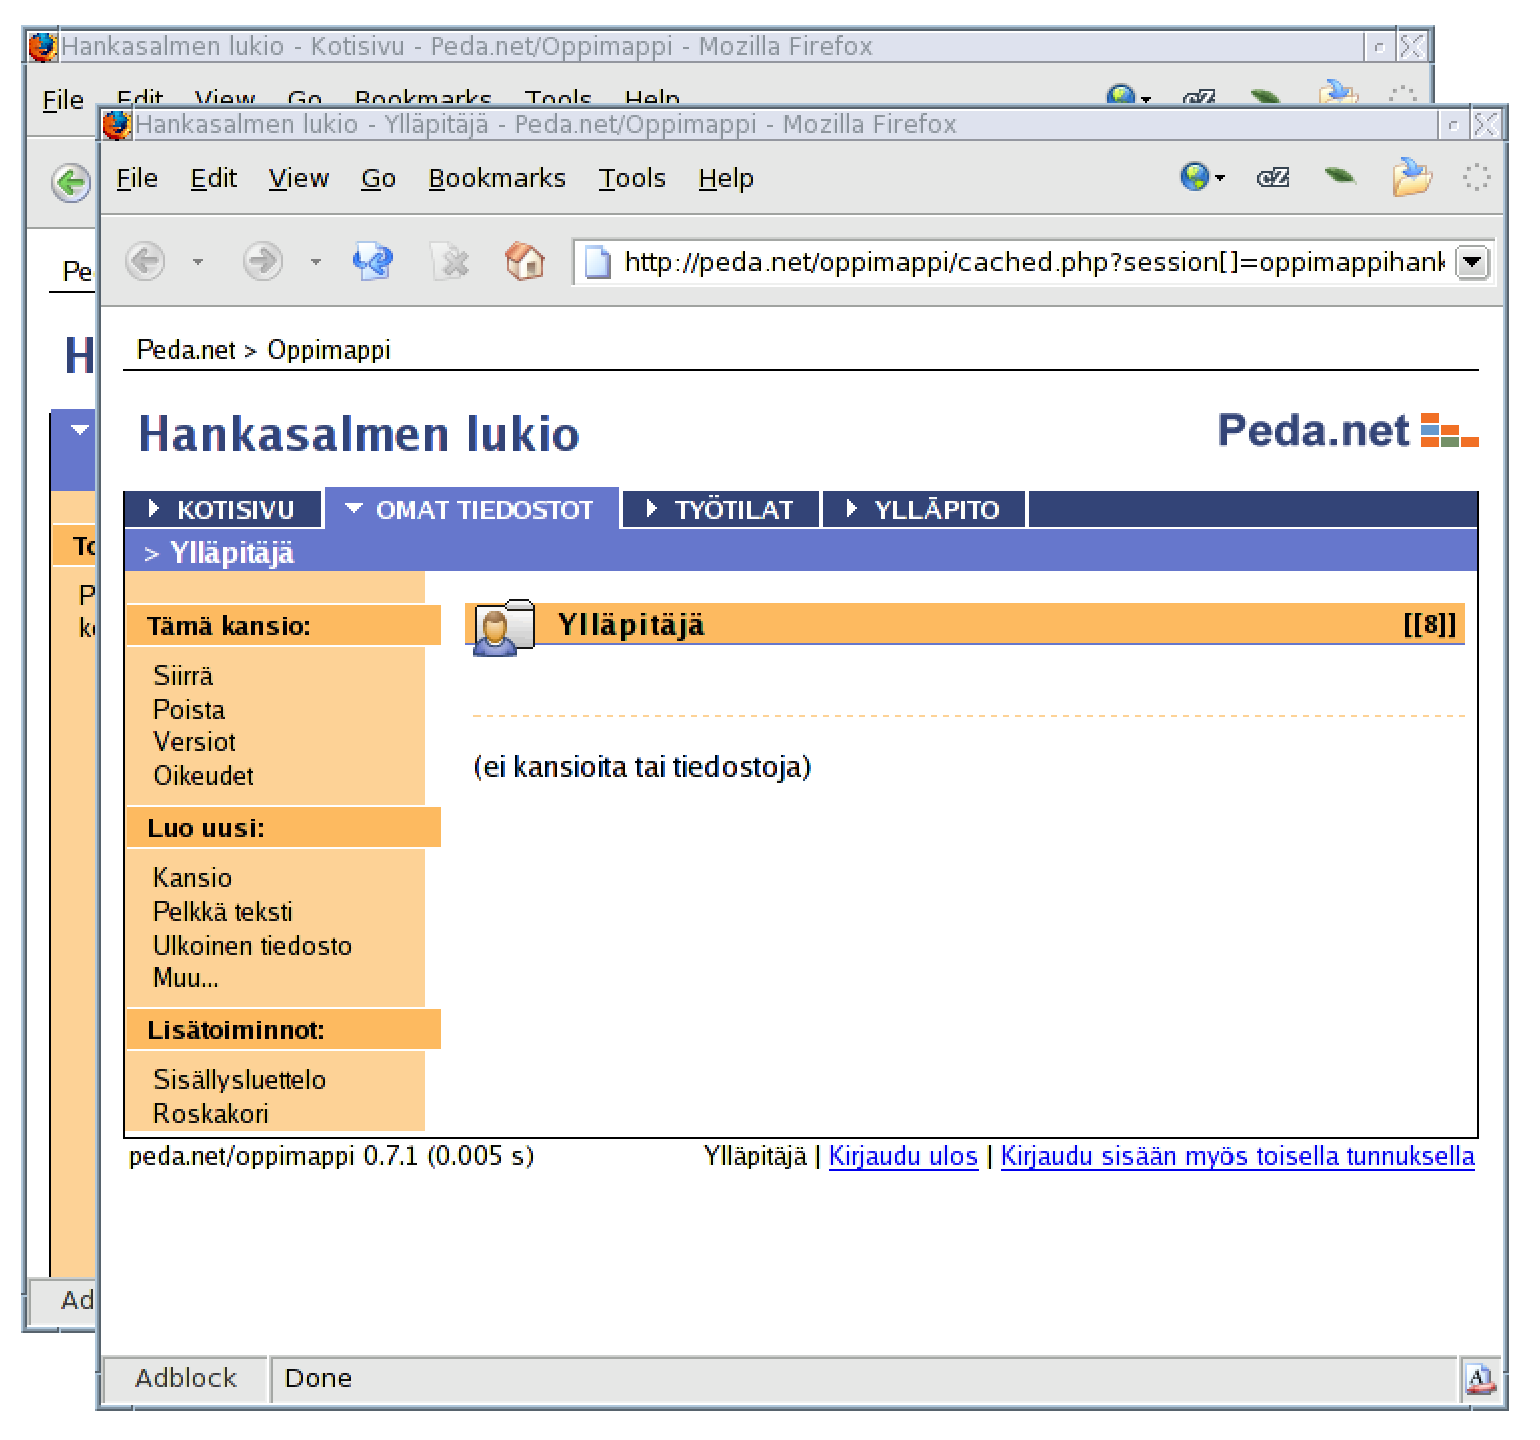
\includegraphics[width=10cm]{kuvat/oppimappi-new-window}
\caption{Oppimappi: linkin avaaminen uudessa ikkunassa}
\label{fig:oppimappi-new-window}
\end{kuva}

Oppimappia voidaan arvioida my�s luvussa
\ref{label:kaytettavyydessa_huomioitavaa} esitettyjen kohtien
perusteella:

\begin{dl}

\item[Ulkon��n taitto:] Oppimapissa oletuksena k�ytetty tyylitiedosto
mukailee Peda.net"-hankkeen staattisia www"-sivuja. Kirjasimeksi on
valittu groteski kirjasinleikkaus, sill� se on yleens� n�yt�ll�
paremmin luettava kuin antiikva. Tekstin kokoa ei ole m��ritelty
absoluuttisesti vaan leip�teksti on k�ytt�j�n selaimen oletuskoko.
Oikein konfiguroitu www"-selain k�ytt�� siis aina optimaalista tekstin
kokoa. K�ytt�j� voi halutessaan k�ytt�� omaa CSS"-tyylitiedostoa.

\item[Yhdenmukaisuus] ja johdonmukaisuus: koko sovelluksen ulkon�k� on
m��ritelty yhdess� CSS"-tyylitiedostossa. Koska HTML"-koodissa ei ole
m��ritelty ulkoasua vaan ainoastaan sis�ll�n rakenne ovat kaikki sivut
kesken��n yhdenmukaisia. Kaikki sis�ll�n muokkaus tapahtuu
toiminta"-palkin kautta ja toiminnot tallennetaan aina lomakkeen
lopussa olevasta ``Tallenna''"-painikkeella. Mik��n, mik� ei n�yt�
painikkeelta ei tee j�rjestelm��n pysyvi�, kaikkia k�ytt�ji� koskevia
muutoksia ja toisaalta kaikkien painikkeiden painaminen tekee pysyvi�
muutoksia. Esimerkiksi ``Poista''"-linkki ei poista tiedostoa
v�litt�m�sti, vaan linkki� painettaessa siirryt��n lomakkeelle, jolla
poisto vahvistetaan painikkeella.

\item[Saavutettavuus:] Oppimapin sis�lt� on esitetty semanttisella
merkinn�ll� ja esimerkiksi sivun ulkoasua ei ole tehty taulukolla.
T�m�n ansioista k�ytt� esimerkiksi puheselaimella onnistuu hyvin.
Samoin kirjasinkokoa voi vapaasti muuttaa ja sovellus k�ytt��
selaimessa asetettua tekstin kokoa. Suurta teksti� tarvitseva k�ytt�j�
on jo aikaisemmin s��t�nyt selaimensa haluamakseen.

\item[Personalisointi:] Oppimappi tarjoaa mahdollisuuden vaihtaa
k�ytt�liittym�n ulkoasua (k�ytt�j� voi valita ulkon��n vaihtoehtoisista
CSS"-tyylisivuista) ja k�ytt�liittym�n kielt�. Lis�ksi j�rjestelm� ker��
tapahtumahistoriaa k�ytt�jien toimista.

\item[Tehokkuus:] Oppimapin vasteaika on keskim��rin 0,04 sekuntia
sivua kohden. Keskim��r�inen sivu on noin 20 kilotavua, mutta
tiedonsiirrossa k�ytet��n gzip"-pakkausta, jos selain sit� tukee, jonka
ansiosta siirrett�v�n datan m��r� on noin 3 kilotavua sivua kohden.
Tavallisella modeemillakin sivun pit�isi siis saapua aina alle 2
sekunnissa. Sivun ulkon�k��n vaikuttava CSS"-tiedosto ja ikonit
tarvitsee siirt�� vain ensimm�isell� sivulla, sen j�lkeen ne ovat
selaimen v�limuistissa. Sovelluksen k�yt�n tehokkuutta on parannettu
tarpeen mukaan nostamalla yleisimmin k�ytettyj� dokumenttien toimintoja
my�s dokumenttien listauksiin, jolloin niiden k�ytt��n tarvitaan yksi sivunhaku v�hemm�n.

\item[Sis�lt�:] Peda.net ei ota kantaa Oppimapilla tuotettavaan
sis�lt��n. K�ytt�liittym�n tekstit yll�pidet��n keskitetysti Peda.netin
toimesta ja eri kieliversioita tehd��n k�ytt�jien tarpeiden mukaan.
Useimmissa tapauksissa joku Peda.netin k�ytt�jist� tarjoutuu
k��nt�m��n tarvittavat merkkijonot uuden kielen tukemista varten.

\item[Luotettavuus:] Oppimappi ei ole ollut viel� k�yt�ss� riitt�v�n
kauan, ett� toimintavarmuudesta voitaisiin sanoa mit��n tarkkaa.
Kuormitustestiss� j�rjestelm� pystyy nykyisell� palvelimella tarjoamaan
l�hes 30 sivua sekunnissa jatkuvasti. J�rjestelm� on ollut t�t�
kirjoitettaessa tuotantok�yt�ss� kaksi viikkoa ilman huoltotaukoja.

\item[Navigointi:] Oppimappi tarjoaa koko ajan linkit koko hierarkian
p��tasoille (kotisivu, omat tiedostot, ty�tilat ja yll�pito) ja muuten
hierarkiassa edet��n yksi taso kerrallaan alasp�in tai palaamalla
suoraan mille tahansa edelliselle tasolle. Kaikki sis�ll�ss� olevat
linkit ovat sinisi� ja alleviivattuja, joten ne on helppo havaita.

\end{dl}

%\section{Johtop��t�ksi� Oppimapin k�ytett�vyydest�}
\label{oppimapin-kaytettavyys-yhteenveto}

Yhteenvetona vaikuttaisi silt�, ett� k�ytett�vyyden kannalta ainakin
CSS"-tyylisivuja pit�isi viel� kehitt��. Erityisesti ikkunan pinta"-ala
on nyt tehottomassa k�yt�ss�, mutta sen korjaamiseksi t�ytyisi poiketa
usein k�ytetyst� www"-sivustojen taitosta. On vaikea sanoa ilman
tarkempaa tutkimusta, onko k�ytett�vyyden kannalta parempi, ett� sivu
n�ytt�� samanlaiselta kuin muutkin, vai ett� sen k�yt�n tehokkuus on
teoriassa maksimaalinen. Samoin k�ytett�vyytt� puheselaimilla ja
braille"-n�yt�ill� pit�isi tutkia viel� tarkemmin.

Toiminnallisesti Oppimapissa on puutteena my�s t�ysi rinnakkaisten
muutosten hallinta. Tietokantaan tehd��n lukituksia vain tiedon eheyden
varmistamiseksi tallennuksen yhteydess�, mutta tiedostoa ei lukita koko
muokkauksen ajaksi. Etuna on, ett� mit� tahansa tiedostoa voi muokata
milloin tahansa, mutta jos samaa dokumenttia muokkaa samaan aikaan
kaksi eri henkil��, eiv�t muutokset yhdisty automaattisesti. Ainoastaan
viimeisen� tallennettu versio j�� voimaan. Versionhallinnan ansiosta
vanhempikin versio tallentuu j�rjestelm��n, mutta muutoksien
yhdist�minen pit�� tehd� j�lkik�teen k�sity�n�. Koska j�rjestelm� pit��
kirjaa my�s vanhoista versioista, tulevaisuudessa on mahdollista tehd�
koneellinen muutosten yhdist�minen, jos eri henkil�iden tekem�t
muutokset eiv�t ole ristiriidassa kesken��n. Selaink�ytt�liittym�n
kehitt�minen ristiriitaisten muutosten yhdist�miseen tulee olemaan
haastava teht�v�. \cite{ritcher:three-way-merge}

Yleisemp�n� ongelmana on rinnakkaisissa muutoksissa tilanne, jossa
henkil� $A$ aloittaa dokumentin muokkaamisen ja t�m�n j�lkeen henkil�
$B$ poistaa saman dokumentin. Jos $A$ nyt yritt�� tallentaa tekem�ns�
muutokset, niin haluttu tulos ei ole itsest��n selv�. Oppimappi ei
toistaiseksi osaa k�sitell� tilannetta, jossa dokumentin muutokset
yritet��n tallentaa, mutta dokumenttia ei ole en�� olemassa. N�in
tapahtuessa k�ytt�j�lle annetaan vain virheilmoitus, jossa toistetaan
k�ytt�j�n sy�tt�m� tieto, jotta h�n voi kopioida sen talteen toiseen
paikkaan. Ongelmana on, pit�isik� j�rjestelm�n palauttaa poistettu
dokumentti j�rjestelm��n. Jos t�m�n pit�� olla mahdollista, ei
j�rjestelm� voikaan koskaan poistaa dokumenttia oikeasti, ainoastaan
piilottaa se n�kyvist�. Vaihtoehtoisesti muokattu sis�lt� voitaisiin
tallentaa uudeksi tiedostoksi. T�ss� mallissa ongelmana on, mihin uusi
tiedosto pit�isi luoda? My�s hakemisto, jossa tiedosto oli, on voitu
poistaa.



\chapter{Pohdintaa}

Tutkimuksen alkuper�inen tavoite oli kehitt�� selaink�ytt�isten
sovellusten k�ytett�vyytt� ja helpottaa niiden valmistamista. Samoin
tavoitteena oli dokumentoida Peda.net-hankkeen kehityskaarta.
Peda.netin uusin ty�kalu, Oppimappi, onnistuu ratkaisemaan
k�ytett�vyyteen liittyv�t ongelmat HTML-kielen antamissa rajoissa
kohtuullisen hyvin, mutta siin� k�ytetty ratkaisumalli olettaa, ett�
kukin osakokonaisuus on kohtuullisen itsen�inen ja koko k�sitelt�v�
sovellus voidaan \emph{luontevasti} esitt�� puurakenteena tai
kaksisuuntaisena puurakenteena\footnote{Esimerkiksi XML ei voi esitt��
kuin yksinkertaisia puurakenteita, mutta silti sit� voidaan k�ytt��
mink� tahansa tiedon siirt�miseen tai tallentamiseen. Tulee kuitenkin
huomata, ett� XML on huomattavan k�mpel� esitysmuoto tietyn tyyppiselle
tiedolle, esimerkiksi kuville.}. Ratkaisemattomaksi ongelmaksi
vaikuttaa siis j��v�n aidosti selaink�ytt�isten k�ytt�liittymien
suunnittelu yleisell� tasolla -- ainakin kun tavoitteena on yht� aikaa
kohtuullisen helppo sovelluksen toteutus ja hyv� k�ytett�vyys.

Tulevaisuuden tutkimuskohteiksi kannattaisi harkita jotain seuraavista:
\begin{ol}
\item Selaink�ytt�isten sovellusten k�ytett�vyys
\item Lomakepohjaisen k�ytt�liittym�n kuvaaminen tehokkaasti
\end{ol}

Tavallisten www-sivujen k�ytett�vyydest� on kirjoitettu useita kirjoja
ja lukemattomia artikkeleita, mutta selaink�ytt�isten sovellusten
k�ytett�vyydest� ei ole juuri tutkimustuloksia n�kynyt. Monella
selaink�ytt�isi� sovelluksia kehitt�v�ll� sovellussuunnittelijalla
tuntuu olevan uskomus, ett� hyv� selaink�ytt�inen sovellus muistuttaa
mahdollisimman paljon tavallista k�ytt�j�n k�ytt�j�rjestelm�ss�
toimivaa ohjelmaa. Itsekin ajattelin joskus n�in, mutta olen sittemmin
oppinut arvostamaan www-selaimien toimintoja joita tavallisissa
ohjelmissa ei n�e. Omasta mielest�ni k�ytett�vyytt� lis��v�t
takaisin-toiminto, joka on er��nlainen \emph{peruuta}-toiminto -- tosin
t�ll� kertaa lomaketasolla eik� toimintotasolla. Lis�ksi k�ytt�j�n
voidaan olettaa tuntevan\footnote{Onko t�m� oletus oikein? Itse olen
n�hnyt useita k�ytt�ji�, jotka eiv�t selv�sti ole ymm�rt�neet
www-selaimen k�ytt�mallia ja viel� v�hemm�n he ovat osanneet k�ytt��
omaa www-selaintaan tehokkaasti.} k�ytt�m�ns� selaimen
erityistoimintoja, jotka nopeuttavat tiedonhankintaa ja sivujen v�lill�
navigointia. Eri sivujen ja dialogien v�lill� tulisi siis siirty�
tavallisten www-sivujen tapaan. Vastakohtana tavalliset,
k�ytt�j�rjestelm�ss� toimivat sovellukset harvoin k�ytt�v�t useita
dialogeja per�kk�in ja eiv�t siten sovellu selaink�ytt�isen sovelluksen
esimerkiksi. Useimmat ``tavalliset'' ohjelmat muokkaavatkin usein
\emph{sen hetkist�} dialogia sen sijasta, ett� n�ytt�isiv�t k�ytt�j�n
toimien tulokset uudessa dialogissa tai sivussa, kuten www-sivut
toimivat.

Toinen t�rke� tutkimuskohde on kuinka lomakepohjaisia k�ytt�liittymi�
voitaisiin kuvata tehokkaasti. Erityisesti tulisi tutkia tarkemmin,
kuinka erilaiset k�sitelt�v�t ongelmat voidaan esitt�� lomakkeilla,
joilla ei ole suoraa yhteytt� k�sittelylogiikkaan. Nykyisin vallalla
oleva malli on t�ss�kin matkia tavallisia sovelluksia ja v�ltt��
yhteydett�myyden ongelmat hakemalla koko lomake aina uudelleen ja
uudelleen, vaikka lomakkeesta muuttuu vain pieni� osia. Erityisesti
tulisi painottua sellaisien ratkaisumallien etsimiseen, jotka eiv�t
vaadi, ett� asiakassovellus (selain) suorittaisi mit��n palvelimen
tarjoamaa ohjelmakoodia tai skriptej� -- toiminnallisuus pit�isi pysty�
toteuttamaan HTML-kielen ja HTTP-protokollan ehdoilla.


\termlist

\begin{terms}

\item[selain] (en. \alt{Browser} tai \alt{User Agent}) on ohjelma,
jolla k�sitell��n verkossa olevaa materiaalia. Selaimen teht�v� on
esitt�� materiaali  k�vij�lle helpoiten k�sitelt�v�ss� muodossa.
Esimerkiksi sokean k�ytt�j�n selain voisi muuntaa kirjoitetun tekstin
��neksi. Yleisin selain t�t� kirjoittaessa on Microsoft Internet
Explorer, vaikka my�s Google"-hakupalvelun Googlebot"-ohjelmaa voisi
v�itt�� viel�kin yleisemm�ksi. Sill�h�n luetaan melkein kaikki
julkisessa verkossa oleva sivut.

\item[semanttinen merkint�] tai merkkaus tarkoittaa sit�, ett�
esimerkiksi HTML"-kielisess� sivussa merkit��n asioiden merkityst� eik�
ulkon�k��. Esimerkiksi sana ``Johdanto'' voidaan merkit�
\emph{otsikoksi}, eik� lihavoiduksi tekstiksi, joka on hieman muuta
teksti� isompaa.

\item[skriptikieli] tarkoittaa ohjelmointikielt�, mutta puhuttaessa
skriptikielest� tarkoitetaan yleens� kielt�, joka on liitetty suoraan
muun sis�ll�n yhteyteen. Yleens� skriptikielen ilmaisuvoima on pienempi
kuin t�yden ohjelmointikielen -- usein esimerkiksi muiden tiedostojen
avaaminen tai muokkaaminen ei ole mahdollista. 

\item[ohjelman tila] on tietokoneohjelman se osa, joka sis�lt�� kaiken
ohjelman tarvitseman tiedon. Esimerkiksi tekstink�sittelyohjelman
tapauksessa tila sis�lt�isi muokattavan tekstin lis�ksi mm. kohdistimen
sijainnin ja ty�kalupalkkien sijaintitiedon.

\item[tapahtuma] on ohjelmoinnissa k�ytetty malli, jossa ohjelman tilaa
ohjaillaan tilaa muuttavilla tapahtumilla. Esimerkiksi ''nappula $A$
painettiin alas'' voisi olla tapahtuma. Tapahtumien vahvuutena on, ett�
sama tapahtuma voidaan tuottaa monessa eri paikassa, mutta tapahtuma
tarvitsee k�sitell� vain yhdess� paikassa -- kun k�sittelyyn tarvitaan
muutoksia, tarvitsee muutos tehd� vain yhdess� paikassa.

\item[HTTP] tai HyperText Transfer Protocol on sarjamuotoinen
protokolla tiedostojen siirt�miseen. Nimens� mukaisesti t�m� protokolla
suunniteltiin alunperin hypertekstin siirt�miseksi, mutta my�hemmin sen
k�ytt� on laajennettu kaikkeen tiedonsiirtoon. Yleisimmin
HTTP-yhteyksi� k�ytet��n TCP/IP"-verkkoyhteyden p��ll�.

\item[HTML] tai HyperText Markup Language on tekstimuotoinen esitystapa
rakenteisen dokumentin esitt�miseen.

\item[XHTML] tai Extensible HyperText Markup Language on HTML-kielen
XML-kielinen versio, jolla kirjoitetuissa dokumenteissa voidaan k�ytt��
my�s muita XML-kielen sovelluksia. XHTML"-kielell� kirjoitetussa
dokumentissa voidaan esimerkiksi k�ytt�� MathML-kielt� matemaattisten
merkint�jen tekemiseen muun tekstin seassa.


\end{terms}


\chapter*{Kiitokset}

Jaana Kettunen ja Juha Lahti auttoivat Peda.netin historian ja eri
tapahtumien vuosilukujen selvitt�misess�. Jaana Kettunen ja P�ivi
Alavuotunki oikolukivat tutkielman. Matthieu Weber ja Antti"-Juhani
Kaijanaho olivat tuottaneet \LaTeX{}"-dokumenttiluokan Pro Gradu
"=tut\-ki\-el\-mia varten, jonka muokattua versiota my�s t�m� dokumentti
k�ytt��. Kiitokset heille!


%%%%%%%%%%%%%%%%%%%%%%%%%%%%%%%%%%%%%%%%%%%%%%%%%%
%	B I B L I O G R A P H Y
%%%%%%%%%%%%%%%%%%%%%%%%%%%%%%%%%%%%%%%%%%%%%%%%%%

\bibliography{bibliography}
\bibliographystyle{bibtexstyle}
%\bibliographystyle{alpha}
%\bibliographystyle{astron}

\end{document}
